\documentclass[type=master]{thuthesis}
% 选项:
%   type=[bachelor|master|doctor|postdoctor], % 必选
%   secret,                                   % 可选
%   pifootnote,                               % 可选(建议打开)
%   openany|openright,                        % 可选,基本不用
%   arial,                                    % 可选,基本不用
%   arialtoc,                                 % 可选,基本不用
%   arialtitle                                % 可选,基本不用

% 所有其它可能用到的包都统一放到这里了,可以根据自己的实际添加或者删除。
\usepackage{thuthesis}

% add by zsshi
\usepackage{array}
\usepackage{multirow}
\usepackage{arydshln}
\usepackage{caption,subcaption}
\usepackage{makecell}
\newcommand{\tabincell}[2]{\begin{tabular}{@{}#1@{}}#2\end{tabular}}
\newcolumntype{P}[1]{>{\centering\arraybackslash}p{#1}}
\newcolumntype{M}[1]{>{\centering\arraybackslash}m{#1}}
\captionsetup{compatibility=false}

\usepackage{bbm}
\usepackage{dsfont}
\usepackage[bb=boondox]{mathalfa}
\DeclareMathAlphabet{\mymathbb}{U}{BOONDOX-ds}{m}{n}
\DeclareMathOperator{\ReLU}{ReLU}
\DeclareMathOperator{\BatchNorm}{BatchNorm}
\DeclareMathOperator{\Sigmoid}{Sigmoid}
\DeclareMathOperator{\Conv3D}{Conv3D}
\DeclareMathOperator{\Maxpooling}{Maxpooling}
\DeclareMathOperator{\Interpolation}{Interpolation}
\DeclareMathOperator*{\Concat}{Concat}
\DeclareMathOperator{\Avgpooling}{Avgpooling}
\makeatletter
\newcommand*\bigcdot{\mathpalette\bigcdot@{.5}}
\newcommand*\bigcdot@[2]{\mathbin{\vcenter{\hbox{\scalebox{#2}{$\m@th#1\bullet$}}}}}
\makeatother

% 定义所有的图片文件在 figures 子目录下
\graphicspath{{figures/}}

% 可以在这里修改配置文件中的定义。导言区可以使用中文。
% \def\myname{薛瑞尼}

\begin{document}

%%% 封面部分
\frontmatter
\thusetup{
  %******************************
  % 注意:
  %   1. 配置里面不要出现空行
  %   2. 不需要的配置信息可以删除
  %******************************
  %
  % 中国海洋大学研究生学位论文封面
  % 参考:中国海洋大学研究生学位论文书写格式20130307.doc
  % 为避免出现错误,下面保留[清华大学学位论文模板原有定义无需修改],
  % 请直接跳到后面[中国海洋大学学位论文模板部分请根据自己情况修改]。
  %
%%%%%%%%%%%%%%%%%%%%%%[清华大学学位论文模板原有定义无需修改]%%%%%%%%%%%%%%%%%%%%%%%
  %=====
  % 秘级
  %=====
  secretlevel={秘密},
  secretyear={10},
  %
  %=========
  % 中文信息
  %=========
  ctitle={清华大学学位论文 \LaTeX\ 模板\\使用示例文档 v\version},
  cdegree={工学硕士},
  cdepartment={计算机科学与技术系},
  cmajor={计算机科学与技术},
  cauthor={薛瑞尼},
  csupervisor={郑纬民教授},
  cassosupervisor={陈文光教授}, % 副指导老师
  ccosupervisor={某某某教授}, % 联合指导老师
  % 日期自动使用当前时间,若需指定按如下方式修改:
  % cdate={超新星纪元},
  %
  % 博士后专有部分
  cfirstdiscipline={计算机科学与技术},
  cseconddiscipline={系统结构},
  postdoctordate={2009年7月——2011年7月},
  id={编号}, % 可以留空: id={},
  udc={UDC}, % 可以留空
  catalognumber={分类号}, % 可以留空
  %
  %=========
  % 英文信息
  %=========
  etitle={An Introduction to \LaTeX{} Thesis Template of Tsinghua University v\version},
  % 这块比较复杂,需要分情况讨论:
  % 1. 学术型硕士
  %    edegree:必须为Master of Arts或Master of Science(注意大小写)
  %             “哲学、文学、历史学、法学、教育学、艺术学门类,公共管理学科
  %              填写Master of Arts,其它填写Master of Science”
  %    emajor:“获得一级学科授权的学科填写一级学科名称,其它填写二级学科名称”
  % 2. 专业型硕士
  %    edegree:“填写专业学位英文名称全称”
  %    emajor:“工程硕士填写工程领域,其它专业学位不填写此项”
  % 3. 学术型博士
  %    edegree:Doctor of Philosophy(注意大小写)
  %    emajor:“获得一级学科授权的学科填写一级学科名称,其它填写二级学科名称”
  % 4. 专业型博士
  %    edegree:“填写专业学位英文名称全称”
  %    emajor:不填写此项
  edegree={Doctor of Engineering},
  emajor={Computer Science and Technology},
  eauthor={Xue Ruini},
  esupervisor={Professor Zheng Weimin},
  eassosupervisor={Chen Wenguang},
  % 日期自动生成,若需指定按如下方式修改:
  % edate={December, 2005}
  %
  % 关键词用“英文逗号”分割
  ckeywords={\TeX, \LaTeX, CJK, 模板, 论文},
  ekeywords={\TeX, \LaTeX, CJK, template, thesis}
}

% 定义中英文摘要和关键字
\begin{cabstract}
  论文的摘要是对论文研究内容和成果的高度概括。摘要应对论文所研究的问题及其研究目
  的进行描述,对研究方法和过程进行简单介绍,对研究成果和所得结论进行概括。摘要应
  具有独立性和自明性,其内容应包含与论文全文同等量的主要信息。使读者即使不阅读全
  文,通过摘要就能了解论文的总体内容和主要成果。

  论文摘要的书写应力求精确、简明。切忌写成对论文书写内容进行提要的形式,尤其要避
  免“第 1 章……;第 2 章……;……”这种或类似的陈述方式。

  本文介绍清华大学论文模板 \thuthesis{} 的使用方法。本模板符合学校的本科、硕士、
  博士论文格式要求。

  本文的创新点主要有:
  \begin{itemize}
    \item 用例子来解释模板的使用方法;
    \item 用废话来填充无关紧要的部分;
    \item 一边学习摸索一边编写新代码。
  \end{itemize}

  关键词是为了文献标引工作、用以表示全文主要内容信息的单词或术语。关键词不超过 5
  个,每个关键词中间用分号分隔。(模板作者注:关键词分隔符不用考虑,模板会自动处
  理。英文关键词同理。)
\end{cabstract}

% 如果习惯关键字跟在摘要文字后面,可以用直接命令来设置,如下:
% \ckeywords{\TeX, \LaTeX, CJK, 模板, 论文}

\begin{eabstract}
   An abstract of a dissertation is a summary and extraction of research work
   and contributions. Included in an abstract should be description of research
   topic and research objective, brief introduction to methodology and research
   process, and summarization of conclusion and contributions of the
   research. An abstract should be characterized by independence and clarity and
   carry identical information with the dissertation. It should be such that the
   general idea and major contributions of the dissertation are conveyed without
   reading the dissertation.

   An abstract should be concise and to the point. It is a misunderstanding to
   make an abstract an outline of the dissertation and words ``the first
   chapter'', ``the second chapter'' and the like should be avoided in the
   abstract.

   Key words are terms used in a dissertation for indexing, reflecting core
   information of the dissertation. An abstract may contain a maximum of 5 key
   words, with semi-colons used in between to separate one another.
\end{eabstract}

% \ekeywords{\TeX, \LaTeX, CJK, template, thesis}
%%%%%%%%%%%%%%%%%%%%%%%%%%%%%%%%%%%%%%%%%%%%%%%%%%%%%%%%%%%%%%%%%%%%%%%%%%%%%%%%

%%%%%%%%%%%%%%%%%%[中国海洋大学学位论文模板部分请根据自己情况修改]%%%%%%%%%%%%%%%%%%%
% 中国海洋大学研究生学位论文封面
% 必须填写的内容包括(其他最好不要修改):
%   分类号、密级、UDC
%   论文中文题目、作者中文姓名
%   论文答辩时间
%   封面感谢语
%   论文英文题目
%   中文摘要、中文关键词
%   英文摘要、英文关键词
%
%%%%%[自定义]%%%%%
\newcommand{\fenleihao}{}%分类号
\newcommand{\miji}{}%密级 
                    % 绝密$\bigstar$20年 
                    % 机密$\bigstar$10年
                    % 秘密$\bigstar$5年
\newcommand{\UDC}{}%UDC
\newcommand{\oucctitle}{基于生成对抗网络的多样式水下图像翻译}%论文中文题目
\ctitle{基于生成对抗网络的多样式水下图像翻译}%必须修改因为页眉中用到
\cauthor{XXX}%可以选择修改因为仅在 pdf 文档信息中用到
\cdegree{工学博士}%可以选择修改因为仅在 pdf 文档信息中用到
\ckeywords{\TeX, \LaTeX, CJK, 模板, 论文}%可以选择修改因为仅在 pdf 文档信息中用到
\newcommand{\ouccauthor}{牛文杰}%作者中文姓名
%\newcommand{\ouccsupervisor}{姬光荣教授}%作者导师中文姓名
%\newcommand{\ouccdegree}{博\hspace{1em}士}%作者申请学位级别
%\newcommand{\ouccmajor}{海洋信息探测与处理}%作者专业名称
%\newcommand{\ouccdateday}{\CJKdigits{\the\year}年\CJKnumber{\the\month}月\CJKnumber{\the\day}日}
%\newcommand{\ouccdate}{\CJKdigits{\the\year}年\CJKnumber{\the\month}月}
\newcommand{\oucdatedefense}{                }%论文答辩时间
%\newcommand{\oucdatedegree}{2009年6月}%学位授予时间
\newcommand{\oucgratitude}{谨以此论文献给我的导师和亲人!}%封面感谢语
\newcommand{\oucetitle}{Underwater Multi-Style Image-to-Image Translation Based on Generative Adversarial Network}%论文英文题目
%\newcommand{\ouceauthor}{Haiyong Zheng}%作者英文姓名
\newcommand{\oucthesis}{\textsc{OUCThesis}}
%%%%%默认自定义命令%%%%%
% 空下划线定义
\newcommand{\oucblankunderline}[1]{\rule[-2pt]{#1}{.7pt}}
\newcommand{\oucunderline}[2]{\underline{\hskip #1 #2 \hskip#1}}

% 论文封面第一页
%%不需要改动%%
\vspace*{5cm}
{\xiaoer\heiti\oucgratitude

\begin{flushright}
---\hspace*{-2mm}---\hspace*{-2mm}---\hspace*{-2mm}---\hspace*{-2mm}---\hspace*{-2mm}---\hspace*{-2mm}---\hspace*{-2mm}---\hspace*{-2mm}---\hspace*{-2mm}---~\ouccauthor
\end{flushright}
}

\newpage

% 论文封面第二页
%%不需要改动%%
\vspace*{1cm}
\begin{center}
  {\xiaoer\heiti\oucctitle}
\end{center}
\vspace{10.7cm}
{\normalsize\songti
\begin{flushright}
{\renewcommand{\arraystretch}{1.3}
  \begin{tabular}{r@{}l}
    学位论文答辩日期:~ & \oucunderline{1.8em}{\oucdatedefense} \\
    指导教师签字:~ & \oucblankunderline{5cm} \\
    答辩委员会成员签字:~ & \oucblankunderline{5cm} \\
    ~ & \oucblankunderline{5cm} \\
    ~ & \oucblankunderline{5cm} \\
    ~ & \oucblankunderline{5cm} \\
    ~ & \oucblankunderline{5cm} \\
    ~ & \oucblankunderline{5cm} \\
    ~ & \oucblankunderline{5cm} \\
  \end{tabular}
}
\end{flushright}
}

\newpage

% 论文封面第三页
%%不需要改动%%
\vspace*{1cm}
\begin{center}
  {\xiaosan\heiti 独\hspace{1em}创\hspace{1em}声\hspace{1em}明}
\end{center}
\par{\normalsize\songti\parindent2em
本人声明所呈交的学位论文是本人在导师指导下进行的研究工作及取得的研究成果。据我所知,除了文中特别加以标注和致谢的地方外,论文中不包含其他人已经发表或撰写过的研究成果,也不包含未获得~\oucblankunderline{7cm}(注:如没有其他需要特别声明的,本栏可空)或其他教育机构的学位或证书使用过的材料。与我一同工作的同志对本研究所做的任何贡献均已在论文中作了明确的说明并表示谢意。
}
\vskip1.5cm
\begin{flushright}{\normalsize\songti
  学位论文作者签名:\hskip2cm 签字日期:\hskip1cm 年 \hskip0.7cm 月\hskip0.7cm 日}
\end{flushright}
\vskip.5cm
{\setlength{\unitlength}{0.1\textwidth}
  \begin{picture}(10, 0.1)
    \multiput(0,0)(0.2, 0){50}{\rule{0.15\unitlength}{.5pt}}
  \end{picture}}
\vskip1cm
\begin{center}
  {\xiaosan\heiti 学位论文版权使用授权书}
\end{center}
\par{\normalsize\songti\parindent2em
本学位论文作者完全了解学校有关保留、使用学位论文的规定,并同意以下事项:
\begin{enumerate}
\item 学校有权保留并向国家有关部门或机构送交论文的复印件和磁盘,允许论文被查阅和借阅。
\item 学校可以将学位论文的全部或部分内容编入有关数据库进行检索,可以采用影印、缩印或扫描等复制手段保存、汇编学位论文。同时授权清华大学“中国学术期刊(光盘版)电子杂志社”用于出版和编入CNKI《中国知识资源总库》,授权中国科学技术信息研究所将本学位论文收录到《中国学位论文全文数据库》。
\end{enumerate}
(保密的学位论文在解密后适用本授权书)
}
\vskip1.5cm
{\parindent0pt\normalsize\songti
学位论文作者签名:\hskip4.2cm\relax%
导师签字:\relax\hspace*{1.2cm}\\
签字日期:\hskip1cm 年\hskip0.7cm 月\hskip0.7cm 日\relax\hfill%
签字日期:\hskip1cm 年\hskip0.7cm 月\hskip0.7cm 日\relax\hspace*{1.2cm}}

\newpage

\pagestyle{plain}
\clearpage\pagenumbering{roman}

% 中文摘要
%%[需要填写:中文摘要、中文关键词]%%
\begin{center}
  {\sanhao[1.5]\heiti\oucctitle\\\vskip7pt 摘\hspace{1em}要}
\end{center}
{\normalsize\songti

习近平同志在党的十九大报告中指出:“坚持陆海统筹,加快建设海洋强国。”水下视觉是海洋研究的基础,在建设海洋强国的今天,水下视觉研究具有重要现实意义、战略意义。由于技术和设备的局限性,水下数据采集耗费巨大、成本高昂,海洋环境中获取特定要求的图像数据困难重重;另一方面由于水下光学物理特性,光在水介质中的传播过程存在吸收和散射,会出现色偏、模糊、有雾状效果等多种样式,却很难获取到指定样式的水下数据。但是目前许多水下图像处理任务,都需要大量成对以及配对的多种样式水下数据。随着深度学习的不断发展,生成对抗网络开始越来越多地被应用于水下视觉研究,逐步为水下图像处理提供了简洁、有效、不受物理模型限制、具有泛化性的方法。

基于生成对抗网络的图像翻译方法在目前水下图像翻译中占据重要的地位,通过了解现有基于生成对抗网络的多样式水下图像翻译问题的国内外现状发现当前的方法还存在缺陷,本工作针对水下图像翻译方法无法同时实现多样式的翻译问题进行了研究和解决。本文主要对水下图像的多样式翻译问题进行了深入的探讨,通过对图像翻译工作进行研究,在图像翻译工作的多模态翻译和多域翻译方向开展实验,提出两种不同思路的模型进行解决。本文主要工作如下:

第一,针对水下图像多样式翻译的问题,我们研究了基于生成对抗网络的图像翻译领域,在充分了解水下图像合成工作后进一步梳理出水下图像多样式翻译可行的两种思路并详尽分析。

第二,一种设计思路是基于跨域图像多模态翻译方法,将多个水下样式看作水下域的多个模态进行处理,提出的水下图像跨域多模态翻译模型引入内容一致性损失限制内容在翻译过程中保持完整不损耗,并对该思路进行具体的网络模型结构设计和目标函数设置。

第三,另一种思路是基于多域翻译的思想进行设计,将包括空中图像在内的各个样式视为多个样式域,把多样式翻译问题建模于多域翻译,通过样式编码控制生成器翻译到各个样式域,并对该设计思路了搭建了具体的网络模型结构和设置了目标函数。

最后,对于设计的水下图像多样式翻译的两种思路,对比图像翻译问题中最经典和最前沿的方法,在多个合成数据集和真实水下数据集上设计了一系列对比实验和消融实验。对每组实验结果进行了详细的评价和分析,定性视觉结果和定量指标结果都验证了我们提出的网络结构可以有效解决水下图像多样式翻译问题,以及得到比现有其它方法更好的结果。
}
\vskip12bp
{\xiaosi\heiti\noindent
关键词:生成对抗网络,图像到图像翻译,多模态翻译,多域翻译,水下图像合成}

\newpage

% 英文摘要
%%[需要填写:英文摘要、英文关键词]%%
\begin{center}
  {\sanhao[1.5]\heiti\oucetitle\\\vskip7pt Abstract}
\end{center}
{\normalsize\songti

Jinping Xi pointed out in the report of the 19th National Congress of the Communist Party of China: Adhere to the overall planning of land and sea, and speed up the construction of a maritime power. Underwater vision is the foundation of marine research. In the time of building a maritime power, underwater vision research has important practical and strategic significance. Due to the limitations of technology and equipment, underwater data collection is expensive and costly, and it is difficult to obtain specific required image data in the marine environment. On the other hand, due to the underwater optical and physical characteristics, there is absorption and scattering in the process of light propagation in the water medium. There will be a variety of styles such as color cast, blur, and foggy effects, but it is difficult to obtain underwater data of the specified styles. However, many underwater image processing tasks currently require a large number of pairs of underwater data in multiple styles. With the continuous development of deep learning, Generative Adversarial Networks(GANs) have begun to be increasingly used in underwater vision research, and gradually provide a concise, effective, and generalized method for underwater image processing that is not restricted by physical models.

The image translation method based on the GANs occupies an important position in the current underwater image synthesis. By understanding the domestic and foreign situation of the existing underwater image multi-style translation based on the generative adversarial network, it is found that the current method still has shortcomings. This work research and solve the problem that underwater image synthesis methods cannot achieve multi-style translation at the same time. The thesis mainly discusses the problem of multi-style synthesis of underwater images. Through the research of image translation, experiments are carried out in the direction of multi-modal translation and multi-domain translation, and two models of different ideas are proposed. The main work of the thesis is as follows:

First, for the problem of underwater image multi-style synthesis, we studied the field of image translation based on GANs. After fully understanding the underwater image synthesis works, we further work out two possible ideas for underwater image multi-style synthesis and analyzed them in detail.

Second, a design idea is based on a cross-domain image multi-modal translation method, which treats multiple underwater styles as multiple modals in the underwater domain, and the proposed underwater image cross-domain multi-modal translation model is introduced the content-consistency loss as the limitation to remain the content intact and not lost during the translation process, and the corresponding network structure design and the function of objective are carried out later.

Third, a design is based on the idea of multi-domain translation, which treats each style including in-air images as multiple style domains, the problem of multi-style is translated to multi-domain translation. The generator translates the input into various style domains,  and it controls the generation through style code. The corresponding network structure and objective are set up for the design idea.

Finally, for the two ideas of designing underwater image multi-style translation, comparing the most classic and the state-of-the-art methods in the image translation problem, a series of comparative experiments and ablation studies were designed on multiple synthetic and real-world underwater datasets. Both qualitative visual results and quantitative metrics results verify that our proposed network can effectively solve the problem of underwater image multi-style translation and obtain better results than other existing methods.

}
 
\vskip12bp
{\xiaosi\heiti\noindent 
\textbf{Keywords: Generative Adversarial Network, Image-to-Image Translation, Multi-Modal Translation, Multi-Domain Translation, Underwater Image Synthesis}}
%%%%%%%%%%%%%%%%%%%%%%%%%%%%%%%%%%%%%%%%%%%%%%%%%%%%%%%%%%%%%%%%%%%%%%%%%%%%%%%%

% 如果使用授权说明扫描页,将可选参数中指定为扫描得到的 PDF 文件名,例如:
% \makecover[scan-auth.pdf]
%\makecover

%% 目录
\tableofcontents

%% 符号对照表
% \begin{denotation}[3cm]
\item[HPC] 高性能计算 (High Performance Computing)
\item[cluster] 集群
\item[Itanium] 安腾
\item[SMP] 对称多处理
\item[API] 应用程序编程接口
\item[PI] 聚酰亚胺
\item[MPI] 聚酰亚胺模型化合物,N-苯基邻苯酰亚胺
\item[PBI] 聚苯并咪唑
\item[MPBI] 聚苯并咪唑模型化合物,N-苯基苯并咪唑
\item[PY] 聚吡咙
\item[PMDA-BDA]	均苯四酸二酐与联苯四胺合成的聚吡咙薄膜
\item[$\Delta G$] 活化自由能 (Activation Free Energy)
\item[$\chi$] 传输系数 (Transmission Coefficient)
\item[$E$] 能量
\item[$m$] 质量
\item[$c$] 光速
\item[$P$] 概率
\item[$T$] 时间
\item[$v$] 速度
\item[劝学] 君子曰:学不可以已。青,取之于蓝,而青于蓝;冰,水为之,而寒于水。木
  直中绳。輮以为轮,其曲中规。虽有槁暴,不复挺者,輮使之然也。故木受绳则直,金就
  砺则利,君子博学而日参省乎己,则知明而行无过矣。吾尝终日而思矣,不如须臾之所学
  也;吾尝跂而望矣,不如登高之博见也。登高而招,臂非加长也,而见者远;顺风而呼,
  声非加疾也,而闻者彰。假舆马者,非利足也,而致千里;假舟楫者,非能水也,而绝江
  河,君子生非异也,善假于物也。积土成山,风雨兴焉;积水成渊,蛟龙生焉;积善成德,
  而神明自得,圣心备焉。故不积跬步,无以至千里;不积小流,无以成江海。骐骥一跃,
  不能十步;驽马十驾,功在不舍。锲而舍之,朽木不折;锲而不舍,金石可镂。蚓无爪牙
  之利,筋骨之强,上食埃土,下饮黄泉,用心一也。蟹六跪而二螯,非蛇鳝之穴无可寄托
  者,用心躁也。—— 荀况
\end{denotation}



%%% 正文部分
\mainmatter
\chapter{绪论}
\section{研究背景和意义}

建设海洋强国是中国特色社会主义事业的重要组成部分。党的十八大报告明确指出,要提高海洋资源开发能力,坚决维护国家海洋权益,建设海洋强国。海洋是生命的摇篮、资源的宝库、交通的命脉、战略的要地。作为海洋研究的重要组成,水下视觉技术在水下机器人设计~\cite{kim2012object,li2020object}、海洋救援任务、海洋生物追踪、实时导航~\cite{chen2012real}等领域中具有广泛应用。水下视觉可以在不具有数据采集条件的条件下为研究者提供必要的技术支持~\cite{ludvigsen2007applications,万媛媛2012水下光视觉目标检测与定位系统关键技术研究},真实水下充满了未知,与陆地视觉研究相比数据采集具有更多的限制。

从生成对抗网络~\cite{goodfellow2014generative}问世开始,计算机视觉领域打开了一个全新的局面,愈来愈多的工作基于生成对抗网络开展。在图像处理领域,可以通过训练简单的基于生成对抗网络的模型合成大量现实中无法获取到但是具有足够真实性的图像数据,其中图像到图像翻译~\cite{isola2017image}被单独划分成一类问题进行解决。图像到图像的翻译简称为图像翻译,图像翻译是指将输入图像“翻译”成一幅相对应的输出图像,输入图像与输出图像之间具有相同或者相类似的内容信息但是具有不同的场景特征。比如翻译成一副对应内容的边缘信息图、语义标签图或者特定场景风格图。我们将这种翻译视为从源域到目标域的映射,输入和输出分别属于两个不同的域。

% 在研究图像翻译问题中,根据可获得的数据集是否包含成对的训练图像可以将解决方法划分为成对的图像翻译子问题和非成对的图像翻译子问题。当数据集满足包含成对的训练图像时,成对的图像翻译问题就可以通过条件生成对抗网络等配对的方法来进行解决。现实情况更多的是不满足获取到大量的成对数据,或者像水下场景等获取成对训练数据特别困难、代价高昂,非成对图像数据的非配对翻译模型被提出。另外,源域和目标域的训练图像数量不平衡,往往一个域中图像数据数量远远超过另一个域图像数据数量,此时给图像翻译带来巨大的难度。

类似我们谷歌翻译一句话,翻译器不会改变我们输入的内容和意思,但是可以翻译成英语、法语等其它语种。在图像翻译中,当目标属于多个种类时,目标域就是多个域,从源域到多个目标域的翻译称为多域翻译~\cite{choi2018stargan,choi2020stargan,lee2020drit++}。谷歌翻译器进行翻译时,不同语种之间的翻译很多情况下并不是一一对应的,一个语义内容可以对应多个翻译结果。在图像翻译中,不成对数据上训练的非配对图像翻译模型可以进行一对多的翻译,网络无法固定学习到特定的映射,可以产生多样输出即多模态翻译~\cite{huang2018multimodal,lee2018diverse,lee2020drit++}。多模态翻译和多域翻译工作是图像翻译的两个重要内容以及经典方向。

图像翻译目前已经有大量的应用,现实中的很多问题都可以转换成图像翻译问题进行解决,图像翻译具有强大的应用价值。可以应用于边框图上色~\cite{ghosh2019interactive}、素描画上色~\cite{cao2017unsupervised,nazeri2018image}等任务,极大的解放了人力;可以应用于图像超分辨重建任务~\cite{ledig2017photo,zhang2019ranksrgan,anokhin2020high},提升图像质量~\cite{wang2019discriminative,bowles2018gan};可以应用于人脸表情漫画化~\cite{yi2019apdrawinggan,shi2019warpgan}、人体姿态图像编辑~\cite{chan2019everybody,cao2019improving}等,实现特定风格的图像生成和控制~\cite{karras2019style},已经落地图像美化等商业软件中;以及在医学图像~\cite{zhou2019prior,lee2019collagan}、水下图像~\cite{uplavikar2019all,li2020underwater}等多种特定学科的常规手段难以直接进行解决的问题中得到应用,给其他学科的图像问题解决提供了新的思路和方法。

在水下环境中,由于采集技术和设备的局限性,整体上在水下环境中的数据采集耗费巨大、成本高昂;另一方面由于水下光学物理特性,光在水介质的传播过程中有吸收和散射,会出现色偏、模糊、有雾状效果等多种样式。然而,对于同一目标却很难获取到大量多样式水下图像数据,许多水下图像处理任务,都需要成对以及多种样式的水下数据。可见,同时获得多种水下环境条件的高质量图像数据对水下图像研究领域意义重大,可以为水下视觉领域提供大量的数据,推动水下研究工作的发展和进步。随着深度学习的广泛发展,生成对抗网络开始越来越多的被应用于水下图像研究,为水下图像处理提供了简洁、有效、不受物理模型限制、具有泛化性的方法。

水下研究中,输入图像与输出图像之间具有相同的内容、不同的场景信息,水下图像合成可称水下图像翻译,在此基础,我们研究基于生成对抗网络的水下图像翻译问题。水下图像翻译与陆地图像翻译不同,会受到许多因素的影响,根据水体光学参数不同,结果呈现出不同的浑浊度和不同的色偏效果。我们提出利用基于生成对抗网络的图像翻译方法处理图像,无需针对多种样式的水下环境考虑水体光学参数和受到物理模型限制。建立在真实水下图像和合成水下图像数据集上,以生成对抗网络作为基础,通过学习水下图像成像特点,将给定的数据转化为多种样式水下数据。在此基础上,还可以探索在指定样式条件下基于生成对抗网络的图像翻译方法进行水下图像翻译。

\section{国内外研究现状}
\subsection{生成对抗网络研究现状}
2014年,在Goodfellow等人~\cite{goodfellow2014generative}提出生成对抗网络(GAN)这项意义深远的工作后,计算机视觉领域的各项工作进入爆发期。生成对抗网络由生成器和判别器组成,生成器试图生成可以欺骗过判别器的真实性结果,判别器负责区分输入的样本是真实样本还是生成器合成的结果。这样处于对抗关系中的两个神经网络彼此不断优化,训练生成器能够生成足够真实的合成结果。

第一个生成对抗网络结构只能应用于相对简单的数据集,这是因为全部使用了全连接神经网络~\cite{goodfellow2014generative}。而卷积神经网络非常适合做图像,Radford等人~\cite{radford2015unsupervised}提出DCGAN,整个模型使用卷积神经网络取代全连接神经网络。CGAN~\cite{mirza2014conditional}将GAN网络拓展至分类条件设置,CGAN对多模态数据生成能够提供更有优势的效果。InfoGAN~\cite{chen2016infogan}将噪声源分解成不可压缩的噪声和潜在编码向量,潜在编码可以用非配对的方式学习目标类。ALI~\cite{donahue2016adversarial}和BiGAN~\cite{zhang2018bidirectional}引入编码器(推理网络),将输入映射到潜在空间向量的推理机制。自动编码器是由编码器和解码器组成网络,编码器从数据空间学习到潜在表示空间的确定性映射,解码器进行从潜在空间到数据空间映射,这两个映射的合成组成重建,并重建结果尽可能接近原始输入。

在研究生成对抗网络时有两个思路,一种是减轻生成对抗网络训练不稳定的问题和模式崩溃问题,另一种是应用于计算机视觉、自然语言处理和其它领域。针对训练不稳定和模式崩溃问题,Mixture Density GAN~\cite{eghbal2019mixture}使用混合密度高斯模型代替原先的模型,分类器除了判别图像的真假外,在嵌入空间中分类器被激励形成多个聚类,判断输入图像属于哪个类型。SRGAN~\cite{liu2019spectral}提出了高斯谱正则化方法,通过对权重矩阵的谱分布进行补偿来防止它们崩溃,进而成功地避免了GAN中的模式崩溃问题。An等人~\cite{an2020ae}提出AE-OT-GAN模型,在生成高质量图像的同时克服了模式崩溃问题。生成对抗网络另一种研究思路是应用于计算机视觉任务,图像合成~\cite{wang2019discriminative}、目标检测~\cite{wang2017fast}、分类和识别~\cite{oza2020multiple,fang2020generate,jung2020icaps}、语义分割~\cite{luc2016semantic}等图像、视频具体任务。

\subsection{图像翻译研究现状}

图像合成包括图像到图像翻译~\cite{isola2017image},文本到图像合成~\cite{zhu2019dm},图像超分辨率~\cite{hyun2020varsr,lee2020journey},去雾去噪~\cite{shao2020domain,wan2020reflection}等。基于生成对抗网络的图像到图像的翻译首次被Isola等人~\cite{isola2017image}在2017年的工作pix2pix中提出,依托条件为图像的条件生成对抗网络思想,训练图像使用尺寸相同的成对数据,是最典型的配对图像翻译方法。同年,Zhu等人~\cite{zhu2017unpaired}提出CycleGAN,基于生成对抗网络提出的循环一致性损失,该方法解决了更普遍没有成对训练数据的非配对图像翻译问题。
% 自此,图像翻译开始被应用于各种具体问题的解决。
DRPAN~\cite{wang2019discriminative}针对图像翻译中的高质量高分辨率合成问题,构建了一个生成对抗网络框架改善合成图像质量,在配对和非配对前沿模型上有效的提升了图像合成质量。

非配对跨域翻译方法中,UNIT~\cite{liu2017unsupervised}将问题定义为实现两个域之间的翻译是满足两个域的联合分布,假设输入到生成器的潜在编码共享,通过编码器将两个域的图像数据编码到潜在空间中。受分解表达学习的影响,MUNIT~\cite{huang2018multimodal}在UNIT提出共享潜在编码的基础上假设潜在编码包括内容编码和风格编码,可以合成内容相同风格不同的多模态结果。DRIT~\cite{lee2018diverse}与MUNIT思路一致,仅在内容编码和风格编码连接方式上有所区别。以上基于分解表示的图像翻译方法广泛应用于风格迁移和多种多模态图像翻译任务中。DSMAP~\cite{chang2020domain}在MUNIT基础上利用特定于域的映射将共享内容空间中的潜在特征重新映射于特定于域的内容空间,这样保证特定于域的内容空间不含有源域的任何信息。

以上方法都是在两个域之间做图像翻译,若要进行多个域之间的翻译需训练多个域间生成器一一对应,StarGAN~\cite{choi2018stargan}用一个生成器结构学习多个域之间的映射从而实现多个域的翻译。StarGAN v2~\cite{choi2020stargan}将StarGAN多域翻译工作拓展至多模态,可以 实现多域多模态的图像翻译任务。在DRIT工作基础上,DRIT++~\cite{lee2020drit++}被提出,除了优化多模态效果外还将两个域之间的翻译也拓展至多个域之间的翻译。


\subsection{水下图像翻译研究现状} 
在研究基于生成对抗网络的水下图像领域时,输入图像与输出图像之间具有相同的内容、不同的场景信息,因此水下图像合成可以称作水下图像翻译。在各种水下图像处理任务中,水下图像数据占据重要地位,有效的水下图像翻译方法研究起着十分关键的作用。水下图像翻译目前主要有以下两种常用的方式,以获得具有真实性的水下图像。

第一种是需要额外的深度图或者传输图等水下信息或基于衰减模型来翻译成具有该特征信息的水下图像翻译方法,主要在室内转水下图像数据集上应用。WaterGAN~\cite{li2017watergan}使用室内Kinect数据集进行翻译,四个RGB-D~\cite{janoch2013category,lai2014unsupervised,silberman2011indoor,shotton2013scene}数据集提供成对的空中图像和对应的深度图翻译成对齐的真实水下结果。Underwater-GAN~\cite{yu2018underwater}使用基于模型的浑浊度模拟生成网络,收集互联网上的图像作为真值,以翻译成17种不同衰减程度的水下图像。UIE-DAL~\cite{uplavikar2019all}和UWCNN~\cite{li2020underwater}使用NYU v2~\cite{silberman2012indoor}数据集中传输图作为衰减系数模拟近海岸和海洋里面不同水类型,控制衰减系数来进行10种水类型的图像翻译。这些方法生成的结果需要依赖于水下信息或者水下,对于真实水下采集到的图像数据缺少泛化能力。

另一种是UGAN~
\cite{fabbri2018enhancing}此类利用CycleGAN这个非配对一对一映射的图像翻译方法,一个域是空中图像、另一个域是水下图像,通过循环一致来学习从空中到水下图像的翻译。MLFCGAN~\cite{liu2019mlfCGAN}和Jamadandi等人~\cite{jamadandi2019exemplar}提出的方法等都是用这种方法进行了水下图像翻译,不依赖于任何水下光学模型和任何物理信息。FUnIE-GAN~\cite{islam2020fast}通过相同的方法拓展成包括配对和不配对子集的大规模EUVP数据集。然而基于CycleGAN的方法都是一对一映射,在图像翻译过程中无法同时生成一对多的多模态结果是此类方法存在的问题。欲得到多种样式结果,需要多个样式对组成的训练数据进行多组训练。

\section{课题来源}
本课题来源于国家自然科学基金面上项目“ 类别不平衡条件下海洋浮游生物图像精细识别及其原位应用研究”(批准号:61771440)和国家自然科学基金面上项目“ 海洋中小型浮游生物原位光学观测关键技术研究”(批准号:41776113)。


\section{论文内容和安排}
本工作主要内容和章节安排如下:

第一章主要针对生成对抗网络,基于生成对抗网络的图像到图像翻译和水下图像翻译的背景意义,国内外研究现状以及课题来源进行介绍。

第二章介绍了生成对抗网络的基本概念、基于生成对抗网络的主流算法和基于生成对抗网络的图像翻译主流方法,引出水下图像翻译的主流方法。概述了算法概念和原理、网络模型结构及算法优缺点等具体内容。

第三章主要描述了本工作提出的基于生成对抗网络的水下图像跨域多模态翻译模型和基于生成对抗网络的水下图像多样式域翻译模型设计,其中包括问题定义和分析、模型网络结构设计和目标函数设置。随网络模型设计思路以及具体的模型实现细节做了详细展现。

第四章介绍了水下图像跨域多模态翻译模型和水下图像多样式域翻译模型的实验和分析评测。对设计的模型进行一系列对比实验和必要的消融实验,充分展示各个模型的实验效果,并将实验结果进行定性和定量分析。

第五章对本工作进行贡献总结和讨论,分析研究问题的特点以及提出方法的优点和缺点,对研究过程中固有问题进行分析和进一步展望。

% 第六章
\chapter{基于生成对抗网络的图像翻译方法}
\section{生成对抗网络}
\subsection{生成对抗网络原理}
\begin{figure*}[ht]
    \centering
	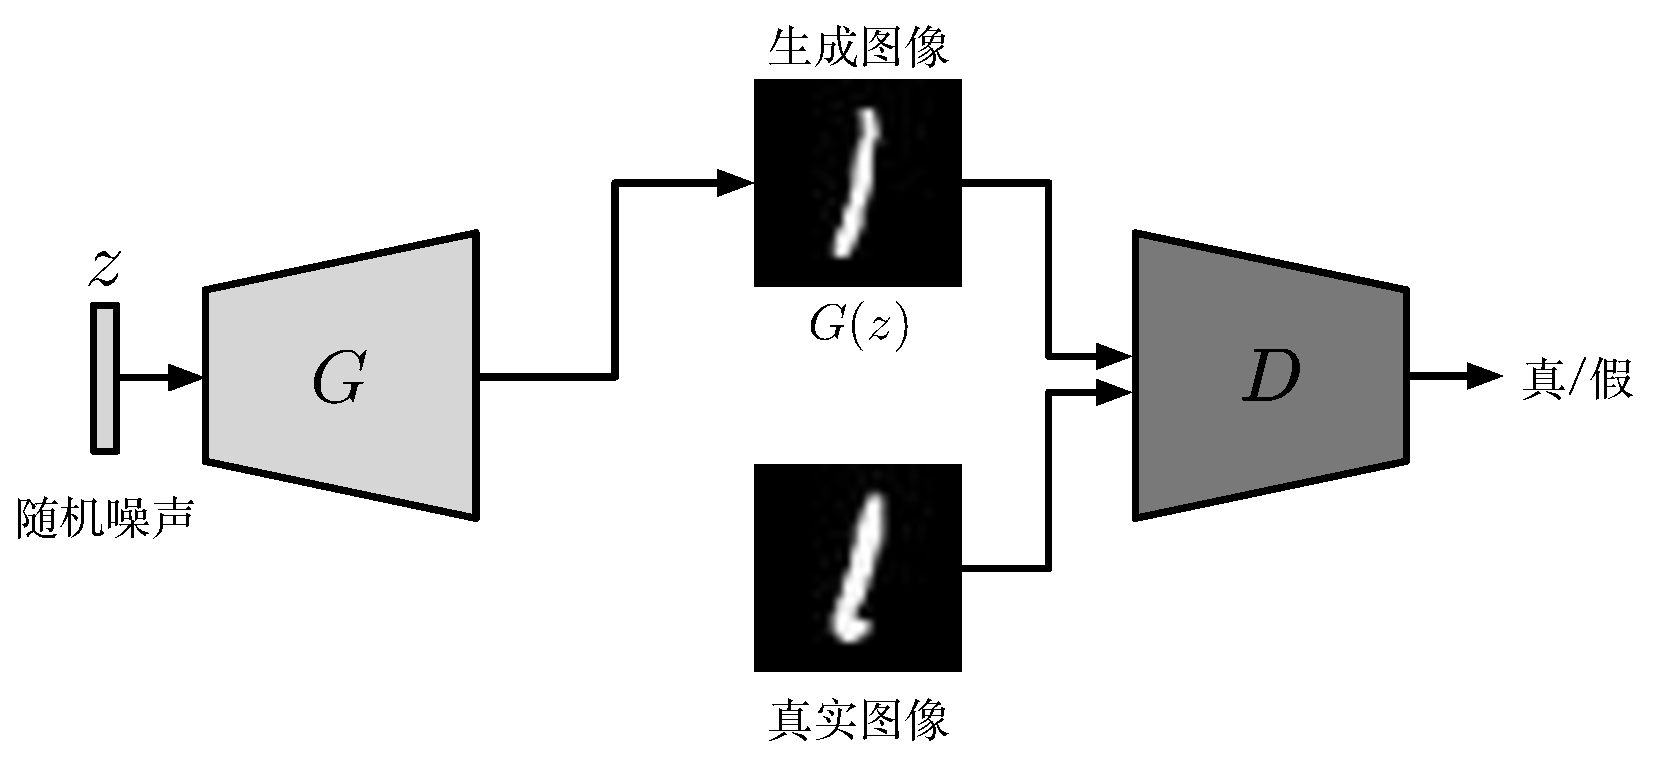
\includegraphics[width=\textwidth]{figures/gan.pdf}
	\caption{生成对抗网络示意图~\cite{goodfellow2014generative}。}
	\label{fig:pic_gan}
\end{figure*}

Goodfellow在2014年提出生成对抗网络(GAN)~\cite{goodfellow2014generative}。生成对抗网络的提出采用二人零和博弈思想,两个神经网络在游戏框架下相互博弈,不断彼此优化,网络结构如图~\ref{fig:pic_gan}所示。由两个彼此独立的神经网络组成:一个生成器$G$,输入随机噪声向量$z$,输出合成数结果据$G(z)$;一个判别器$D$,输入真实数据$x$或者合成数据结果$G(z)$,判别器试图区分输入真实数据还是合成数据。
\begin{equation}
\begin{split}
\mathop{min} \limits_{G} \mathop{max} \limits_{D} \mathbb{E}_{x \sim p_{data}(x)}[\log D(x)] + \mathbb{E}_{z \sim p_{z}(z)}[log(1-D(G(z)]
\end{split}
\label{equ:equ_gan}
\end{equation}

在训练过程中,生成器和判别器分别单独交替训练,目标函数如式~\ref{equ:equ_gan}所示。优化生成器时判别器固定,生成样本当作真实数据优化,$\min \limits_{G}$最小化生成样本和真是样本之间的差异;优化判别器时固定生成器,把生成样本当作虚假数据进行处理,$\max \limits_{D}$尽可能的让判别器最大化的判别出样本来自真实数据还是生成数据。这是博弈得以进行的关键之处,理想情况下生成分布会拟合于真实分布。

生成对抗网络相比较于之前的生成模型的优势有两点。一是因为不依赖任何先验假设,而传统的方法会假设数据服从某一分布,然后用极大似然去估计分布;二是生成类似真实样本的方法简单,直接利用生成器前向传播进行生成。然而,生成对抗网络也有其不可忽视的缺点。训练中有时不收敛,网络不稳定难以训练;模式坍塌问题,生成的缺少多样性的结果。

\subsection{生成对抗网络发展}
本节将对生成对抗网络发展过程中具有里程碑意义的变种模型进行介绍,以及对传统生成对抗网络的问题的优化方法。

\subsubsection{CGAN}

\begin{figure*}[ht]
    \centering
	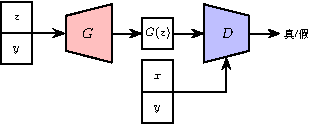
\includegraphics[width=0.8\textwidth]{figures/CGAN.pdf}
	\caption{条件生成对抗网络示意图。图片来自文献~\cite{mirza2014conditional}。}
	\label{fig:pic_CGAN}
\end{figure*}

原始生成对抗网络不能生成具有特定属性的图像结果,针对这个问题,Mirza等人提出条件生成对抗网络(CGAN)~\citep{mirza2014conditional}。如图~\ref{fig:pic_CGAN}所示,核心创新点在于将属性信息$y$融入生成器$G$和判别器$D$中,属性$y$可以是任何标签信息,例如图像的类别信息或者图像本身等。
% CGAN 目标函数
% \mathbf{V}(D,G)  = 
% \begin{equation}
% \label{equ:equ_CGAN}
% \mathop{min} \limits_{G} \mathop{max} \limits_{D} \mathbb{E}_{x \sim p_{data}(x)}[\log D(x|y)] + \mathbb{E}_{z \sim p_{z}(z)}[log(1-D(G(z|y)]
% \end{equation}



\subsubsection{DCGAN}
从Alex Krizhevsky等人创造大型深度卷积神经网络AlexNet~\cite{krizhevsky2017imagenet}赢得2012年ImageNet~\cite{deng2009imagenet} 大规模视觉识别挑战赛ILSVRC开始,卷积神经网络(CNN)在计算机视觉领域成功亮相。2016年,Radford等提出了深度卷积生成对抗网络(DCGAN)~\cite{radford2015unsupervised},使用深度卷积神经网络代替原始GAN中全链接层的线性感知,将网络拓展至层数更深、参数更多的任务中,进而提高了生成样本的质量和收敛的速度。

\begin{figure*}[ht]
    \centering
	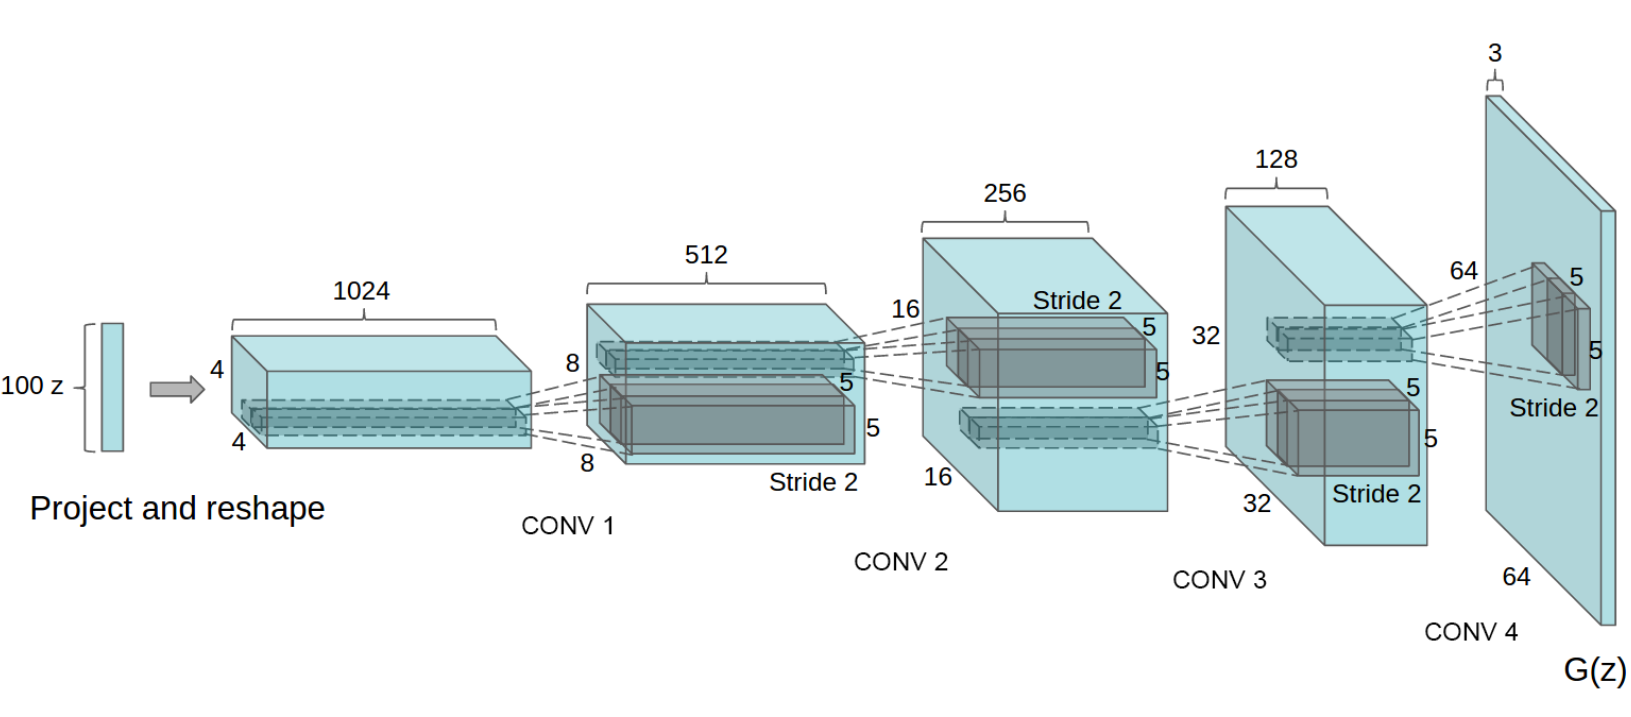
\includegraphics[width=\textwidth]{figures/DCGAN.png}
	\caption{深度卷积生成对抗网络的反卷积过程示意图。图片来自文献~\cite{radford2015unsupervised}。}
	\label{fig:pic_dCGAN}
\end{figure*}

深度卷积生成对抗网络对生成对抗网络的模型结构做了巨大的改进,如图~\ref{fig:pic_dCGAN}所示。创新点如下:(1)在网络结构中取消全链接层,使用全卷积网络。
% 生成器和判别器对称存在,极大的提升了GAN训练稳定和和生成结果质量。
(2)将对抗网络中的池化层取消,使用带步长的卷积层和反卷积层进行上/下采样操作,更好的提取图像特征。(3)在生成器和判别器中使用批归一化(BatchNorm)~\cite{ioffe2015batch}。
% ,为了网络稳定,在生成器输出层和判别器的输入层取消使用批归一化。
(4)生成器中,除了最后一层使用Tanh激活函数外,其余都是ReLU~\cite{nair2010rectified}激活函数。(5)在判别器中,所有层都使用LeakyReLU~\cite{xu2015empirical}激活函数,从而防止梯度稀疏。

% 深度卷积生成对抗网络对生成对抗网络所做的创新,虽然一定程度上稳定了训练,生成较高质量的结果,但是并没有从根本上解决生成对抗网络训练不稳定的问题,在训练过程中仍需要注意生成器和判别器的平衡问题以及模式坍塌问题的出现。

% \subsubsection{LSGAN}
% \begin{figure*}[ht]
%     \centering
% 	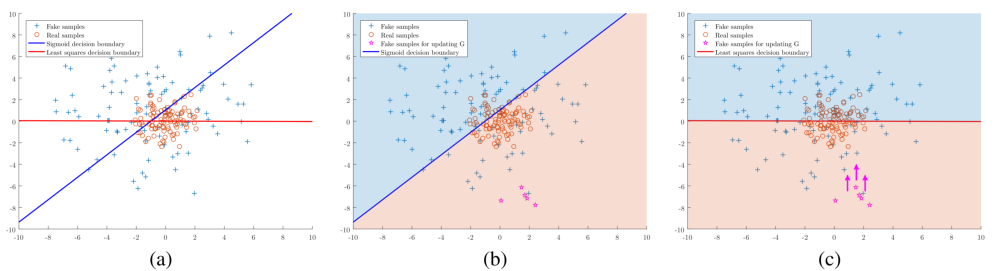
\includegraphics[width=\textwidth]{figures/lsgan.pdf}
% 	\caption{GAN中Sigmoid决策边界LSGAN最小二乘决策边界图示。图片来自文献~\cite{mao2017least}。}
% 	\label{fig:pic_lsgan}
% \end{figure*}

% LSGAN~\cite{mao2017least}针对GAN生成图像质量不高以及训练过程不稳定的问题进行改进,具体来说就是将GAN的目标函数由交叉熵损失换成最小二乘损失。

% 准确的决策边界会穿过真实数据点,把决策边界当作中介,生成图像结果和真实数据之间的距离可以由生成结果和决策边界之间的距离来反映。如图~\ref{fig:pic_lsgan}所示,蓝色十字形状表示假样本数据,红色空心圆圈是真样本数据,蓝色线条是原始GAN中Sigmoid决策边界,红色线条是LSGAN中最小二乘决策边界。(a)是两个损失函数决策边界对比图。在(b)和(c)中,枚红色五星表示更新生成器过程中的加样本数据。如(b)中所示,橘色是真实数据区域,蓝色是加样本区域。若使用交叉熵作为损失,当交叉熵损失很小时,生成器不会再优化那些被生成器识别为真实图片的生成结果,事实上此时这些生成结果距离决策边界也就是真实数据分布依旧很远,生成器却也不再进行优化。如(c)当损失函数为最小二乘损失时,要想最小化最小二乘损失,生成器必然会将距离决策边界也就是真实数据分布的生成结果拉向决策边界。

% LSGAN目标函数定义如式~\ref{equ:equ_lsgan}。%和~\ref{equ:equ_lsgan_g},其中参数设置$a=c=1$,$b=0$
% \begin{equation}
% \begin{split}
% \min\limits_D\frac{1}{2}\mathbb{E}_{x \sim p_{data}(x)}[(D(x)-b)^2]+\frac{1}{2}\mathbb{E}_{z\sim{p_z(z)}}[D(G(z))-a)^2] \\
% \min\limits_G\frac{1}{2}\mathbb{E}_{z \sim{p_z(z)}}[D(G(z))-c)^2]
% \end{split}
% \label{equ:equ_lsgan}
% \end{equation}

% \begin{equation}
% \label{equ:equ_lsgan_g}
% \min \limits_G\frac{1}{2}\mathbb{E}_{z \sim{p_z(z)}}[D(G(z))-c)^2]
% \end{equation}


% \subsubsection{ACGAN}
% \begin{figure*}[ht]
%     \centering
% 	\includegraphics[width=0.4\textwidth]{figures/aCGAN.pdf}
% 	\caption{ACGAN结构示意图。图片来自文献~\cite{odena2017conditional}。}
% 	\label{fig:pic_aCGAN}
% \end{figure*}

% CGAN通过结合标签信息来提高生成数据的质量,ACGAN~\cite{odena2017conditional}除此之外,还通过重建标签信息来提高生成数据的质量。模型结构如图~\ref{fig:pic_aCGAN}所示,生成器的输入是分类标签和固定的噪声分布,判别器的输出除了指示真假的对抗损失外,还出增加一个辅助分类器判别分类标签,输入的标签当作目标进行反馈,提高判别网络的学习效果。

% 目标函数包含两个部分:判别真实性的对抗损失$\mathcal{L}_S$如式~\ref{equ:equ_aCGAN_s}和类别判别损失$\mathcal{L}_C$如式~\ref{equ:equ_aCGAN_c}。其核心贡献对于真实图片Xreal和生成器伪造的图片Xfake,辅助分类器应该能够预测它所属的类别。噪声分布$Z$独立于类别标签$C$;判别器训练中试图最大化$\mathcal{L}_S+\mathcal{L}_C$,而生成器最大化$\mathcal{L}_C-\mathcal{L}_S$。

% \begin{equation}
% \label{equ:equ_aCGAN_s}
% \mathcal{L}_S = \mathbb{E}[\log P(S = real | X_{real})] + \mathbb{E}[logP(S = fake | X_{fake})]
% \end{equation}

% \begin{equation}
% \label{equ:equ_aCGAN_c}
% \mathcal{L}_C = \mathbb{E}[\log P(C = c | X_{real})] + \mathbb{E}[logP(C = c | X_{fake})]
% \end{equation}

% ACGAN的一个作用就是弥补数据的不足,让计算机拥有了能够模仿现有数据从而生成独特数据的能力,用途相当广泛。

% \subsection{Wasserstein GAN}
% 作者Arjovsky提出Wasserstein GAN(WGAN)~\cite{arjovsky2017wasserstein}在Reddit机器学习频道引起热议。该工作在理论上分析了原始GAN的问题和限制,针对这些问题给出改进算法,主要创新点如下:

% (1)彻底解决了GAN训练不稳定的问题,不需要再平衡生成器和判别器的训练程度。

% (2)基本解决了模式坍塌问题,确保生成样本的多样性。

% (3)Wasserstein距离通过数值指示训练进程,数值越小GAN训练越好,生成质量越高。

% (4)不需要精心设计网络架构,简单的多层全连接网络也可实现。

% 在网络结构上,具体改进为:判别器最后一层去掉sigmoid激活函数,判别器最小化Wasserstein距离,缩小生成分布和真实分布的的Wasserstein距离;生成器和判别器的损失函数不进行$log$计算;每次更新判别器的参数之后,将参数绝对值截断至小于固定参数以满足Lipschitz连续条件;使用非基于动量的优化算法,譬如RMSProp,SGD等适合梯度不稳定的情况。

% 目标函数中,判别器试图最小化式~\ref{equ:equ_wgan_d},其中$m>0$,$[x]^x=max(0,x)$
% % WGAN_D 目标函数
% \begin{equation}
% \label{equ:equ_wgan_g}
% \mathop{min} \limits_{D} \mathbb{E}_{x \sim p(x)}[D(x)] + \mathbb{E}_{z \sim p(z)}[[m-D(G(z))]^+]
% \end{equation}

% 生成器试图最小化式~\ref{equ:equ_wgan_g}
% % WGAN_G 目标函数
% \begin{equation}
% \label{equ:equ_wgan_d}
% \mathop{min} \limits_{G} \mathbb{E}_{z \sim p(z)}[D(G(z)] - \mathbb{E}_{x \sim p(x)}[D(x)]
% \end{equation}

% WGAN有时候也会出现生成样本质量低,难以收敛的问题。

% \subsection{WGAN-GP}
% WGAN-GP~\cite{gulrajani2017improved}是WGAN的改进版,改进了原设计中Lipschitz限制的施加方式,加入梯度惩罚让梯度在后向传播的过程中保持平稳。



\section{基于生成对抗网络的图像翻译}
图像翻译旨在通过设计端到端的模型将源域图像转换到目标域图像,通常源域提供图像的内容,目标域提供图像的“风格”(可以是图像属性或图像风格),在源域内容下实现目标域的“风格”化,从而实现源域图像到目标域图像的转换。根据训练中是否需要成对图像即源域图像和目标域图像是否一一对应,可以分为成对图像翻译和非成对图像翻译。


\subsection{成对图像翻译方法}
% 2017年Isola等人提出pix2pix~\cite{isola2017image},是典型的配对训练图像的图像翻译方法。本质上是基于CGAN,将输入图像作为条件,学习从输入图像到输出图像之间的映射,从而得到指定的输出图像。%pix2pix等成对图像翻译方法可以比较清晰的语义图到真实场景图、灰度图上色、日景到夜景、草图到图像等图像的转换结果。
\begin{figure*}[htp]
    \centering
	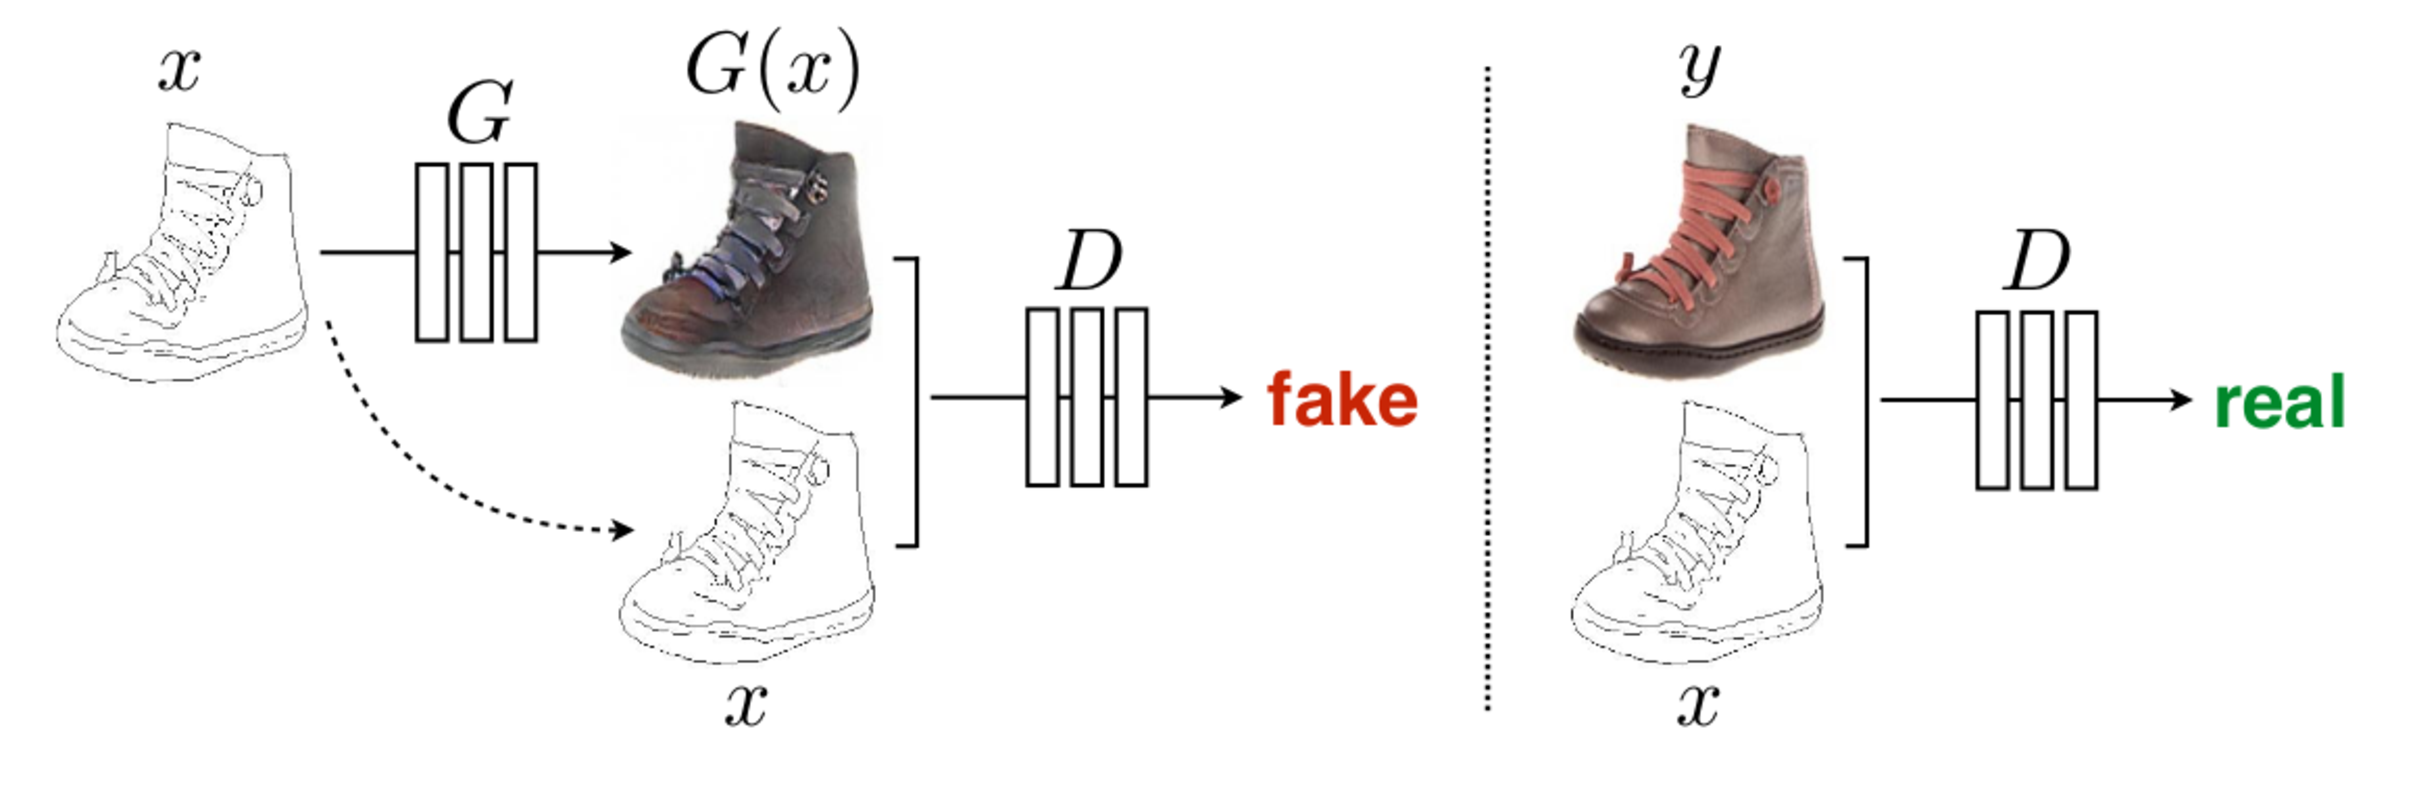
\includegraphics[width=\textwidth]{figures/pix2pix.pdf}
	\caption{pix2pix训练示意图。图片来自文献~\cite{isola2017image}。}
	\label{fig:pix2pix}
\end{figure*}

2017年Isola等人~\cite{isola2017image}提出pix2pix,是典型的配对图像翻译方法。
%本质上是基于CGAN,将输入图像作为条件,学习从输入图像到输出图像之间的映射,从而得到指定的输出图像。
% 以草图到图像的翻译为例,
训练过程如图~\ref{fig:pix2pix}所示。网络结果基于CGAN,将图片$x$作为条件,$y$是跟$x$配对的真实结果,需要输入生成器$G$和判别器$D$中。判别器试图区分合成图像$\{x,G(x)\}$和真实图像$\{x,y\}$,生成器试图生成具有真实性的结果以迷惑判别器。
% 跟无条件GAN不同,pix2pix的生成器和判别器都需要输入条件$x$。
生成器采用U-Net全卷积结构,
% ,跟Encoder-Decoder网络结构先下采样到低维度再上采样到原始分辨率有所区别,
编码过程中对应的特征图和解码之后同样尺寸的特征图按照通道拼接在一起,目的是用来保留不同分辨率下像素级的细节信息。为了更好的对图像局部做判断,判别器利用马尔可夫性的判别器PatchGAN结构。其工作原理是将图像中独立的$N \times N$个patch真假判别,而非将整个图像真假判别,这种设计使得参数更少、运行更快,且能够产生更为锐利的结果。


% \begin{figure*}[ht]
%     \centering
% 	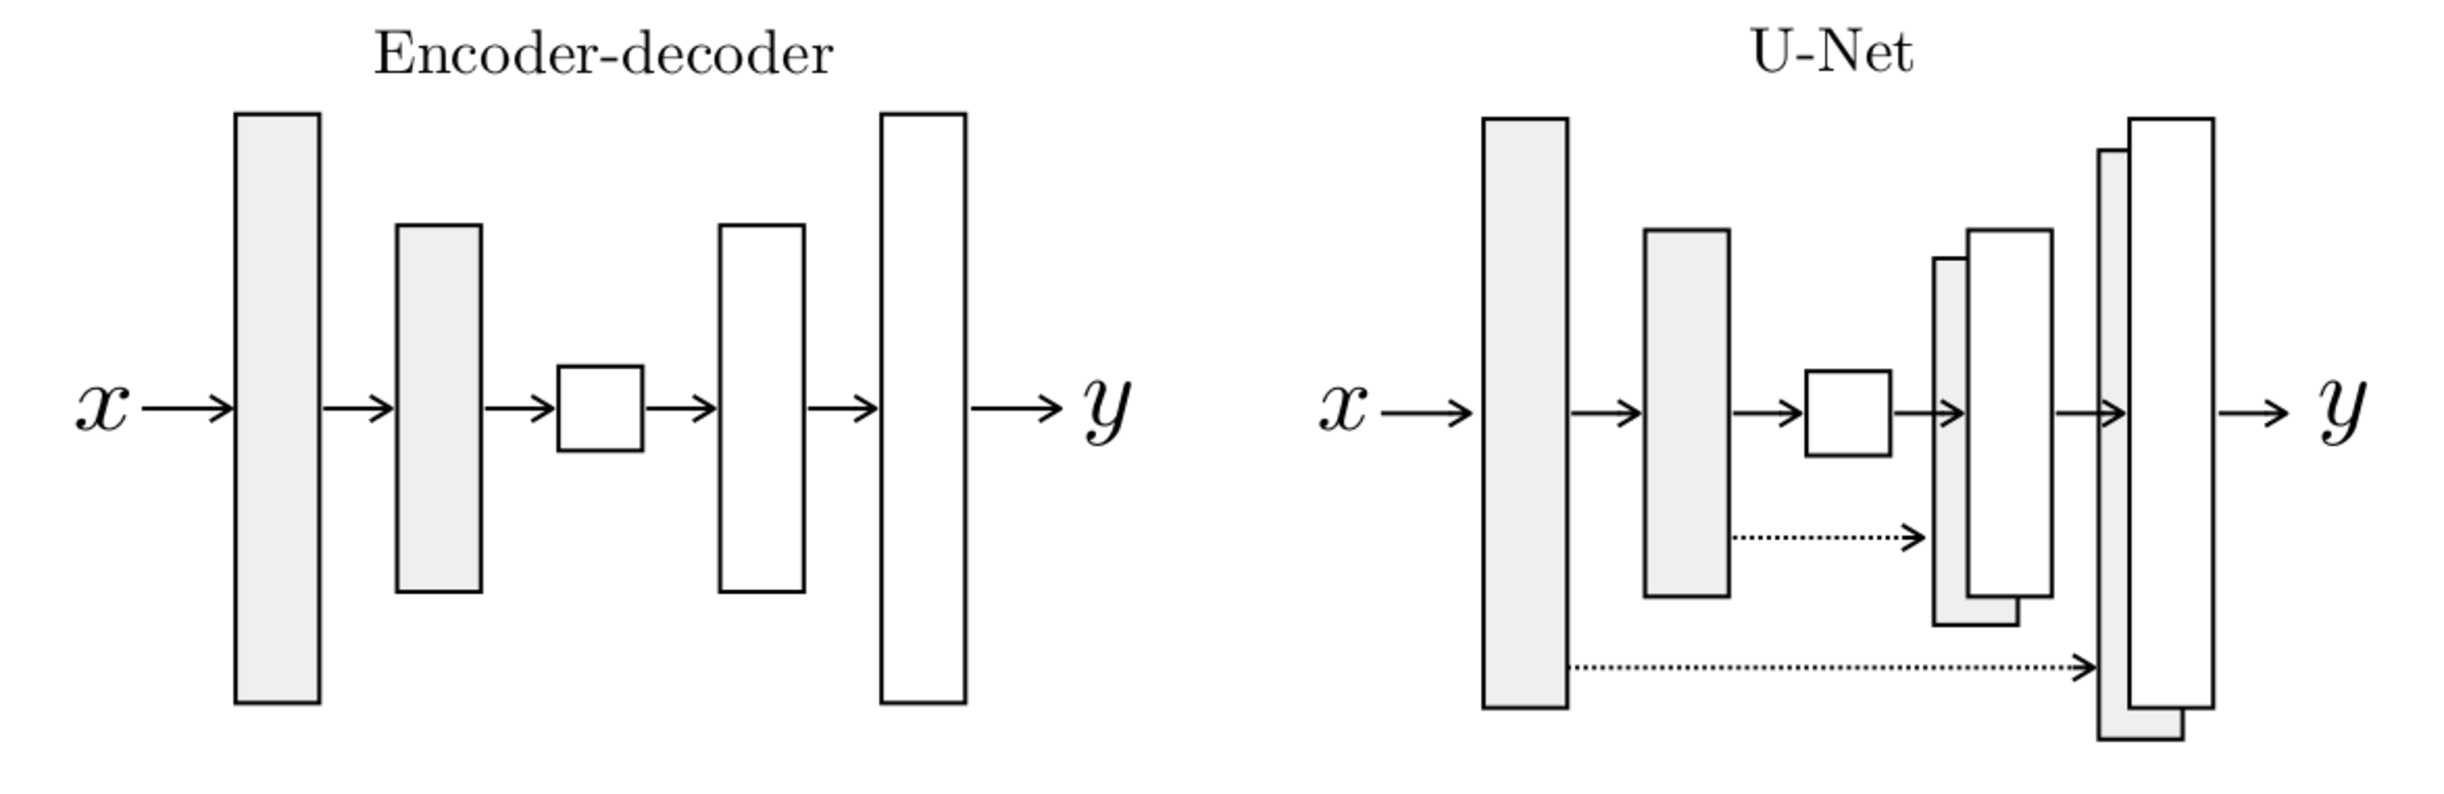
\includegraphics[width=\textwidth]{figures/unet.pdf}
% 	\caption{pix2pix生成器U-net网络结构示意图。}
% 	\label{fig:unet}
% \end{figure*}

% \begin{equation}
% \label{equ:pix2pix_CGAN}
% \mathcal{L}_{CGAN}(G,D) = \mathbb{E}_{x,y}[\log D(x,y)] + \mathbb{E}_{x,z}[\log(1-D(x,G(x,z)))]
% \end{equation}

% pix2pix的生成器和判别器网络结构在DCGAN的深度卷积的基础上做了一些改进。

% 如图~\ref{fig:unet}所示,左侧是Encoder-Decoder网络结构,右侧是U-Net~\cite{ronneberger2015u}结构,区别是加入skip-connection,编码过程中对应的特征图和解码之后同样尺寸的特征图按照通道拼接在一起,目的是用来保留不同分辨率下像素级的细节信息。为了更好的对图像局部做判断,判别器利用马尔可夫性的判别器PatchGAN结构。其工作原理是将图像中独立的$N \times N$个patch真假判别,而非将整个图像真假判别,这种设计使得参数更少、运行更快,且能够产生更为锐利的结果。

% \begin{equation}
% \label{equ:pix2pix_l1}
% \mathcal{L}_{L1}(G) = \mathbb{E}_{x,y,z}[\parallel y-G(x,z) \parallel_1]
% \end{equation}

% \begin{equation}
% \label{equ:pix2pix}
% \min \limits_G \max \limits_D \mathcal{L}_{CGAN}(G,D) + \lambda \mathcal{L}_{L1}(G)
% \end{equation}

% 基于CGAN的目标函数为~\ref{equ:pix2pix_CGAN},$\mathcal{L}_1$损失为~\ref{equ:pix2pix_l1},总目标函数为这两项之和。
% ~\ref{equ:pix2pix}。
% $\mathcal{L}_1$损失可以恢复图像低频部分让生成图像跟真实训练数据尽量相似,对抗损失额可以恢复图像的高频部分细节。

DRPAN~\cite{wang2019discriminative}针对图像翻译中的高质量高分辨率合成问题,创新性的提出了一种基于块的判别 区域候选机制DRPnet,并构建了一个DRPAN生成对抗网络框架改善合成图像质量,可以得到更高 分辨率、具有更真实细节且更少伪影的高质量图像。所提出的DRPnet机制分别在配对模型pix2pixHD~\cite{wang2018high}和非配对模型CycleGAN~\cite{zhu2017unpaired}上都有很好的泛化能力。

\begin{figure*}[ht]
    \centering
	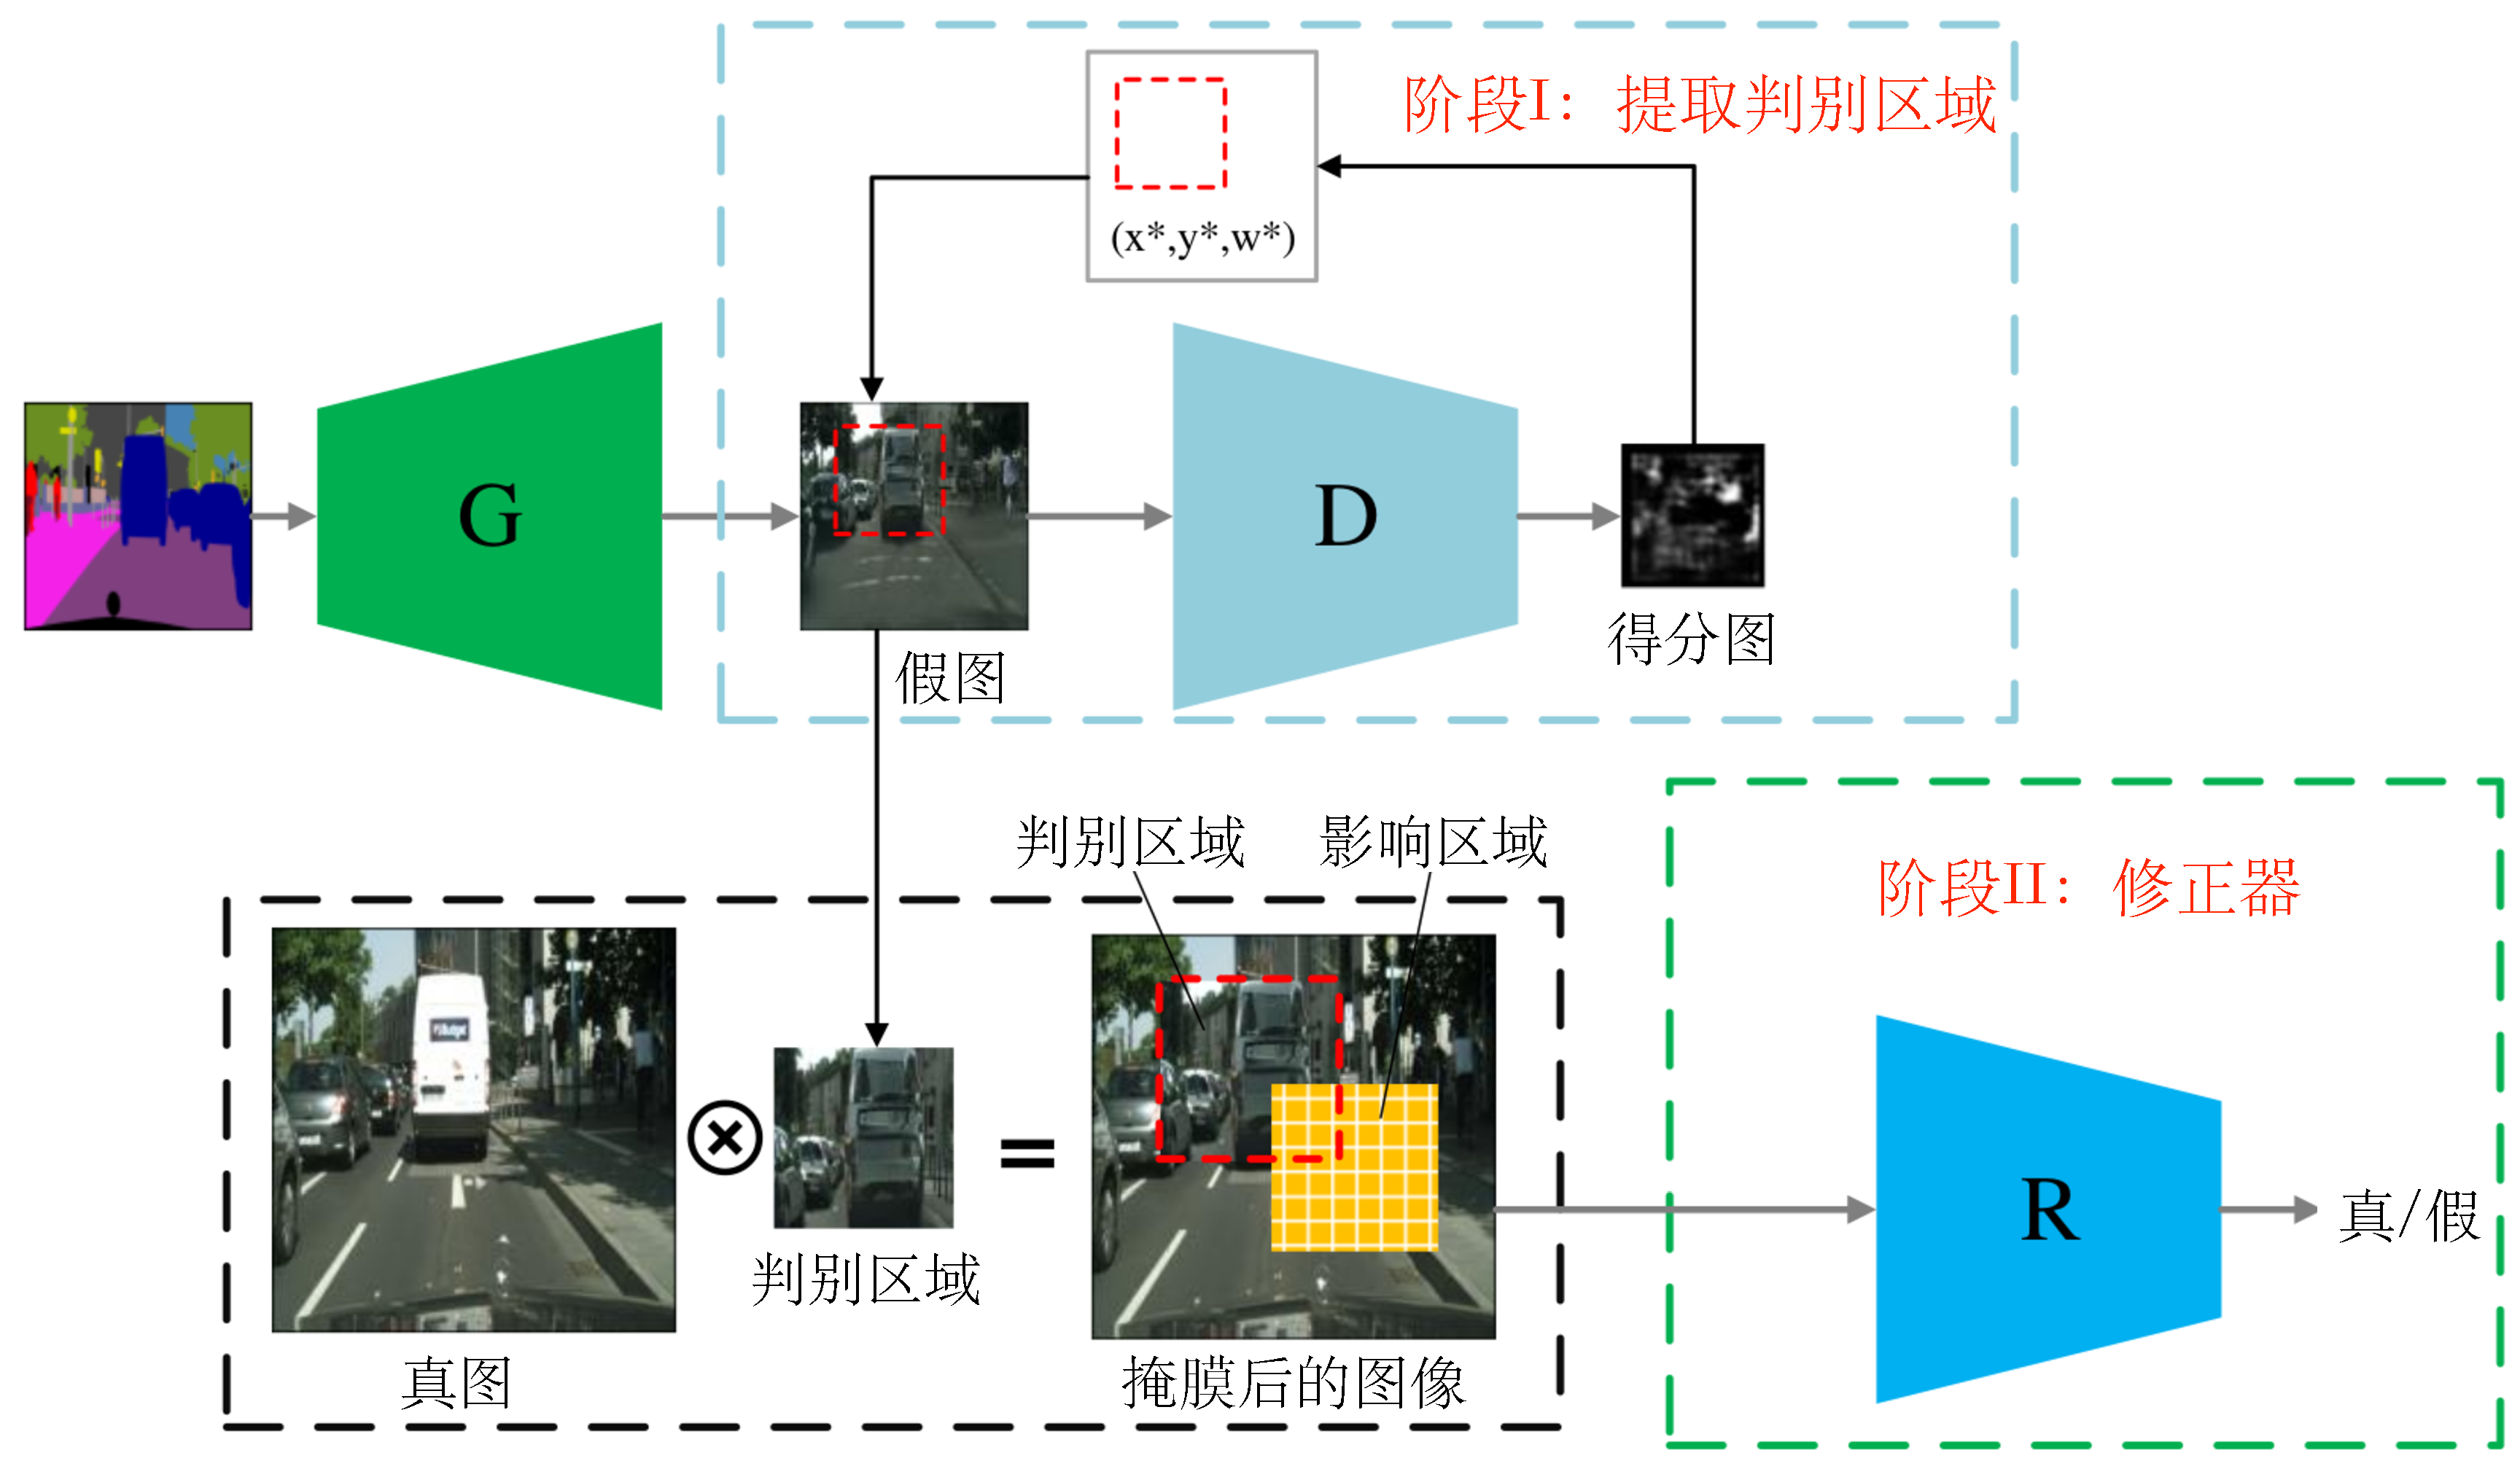
\includegraphics[width=\textwidth]{figures/DRPAN.pdf}
	\caption{DRPAN训练示意图。图片来自文献~\cite{wang2019discriminative}。}
	\label{fig:drpan}
\end{figure*}

\subsection{非成对图像翻译方法}
很多任务中,由于真实数据限制,我们无法得到成对的源域和目标域图像来进行训练,比如将照片翻译成艺术作品风格、人脸翻译成漫画风格等源域和目标域图像没有关联性甚至毫不相干的风格转换任务。由此可见,非成对图像翻译应用场景更加广泛。

\begin{figure*}[ht]
    \centering
	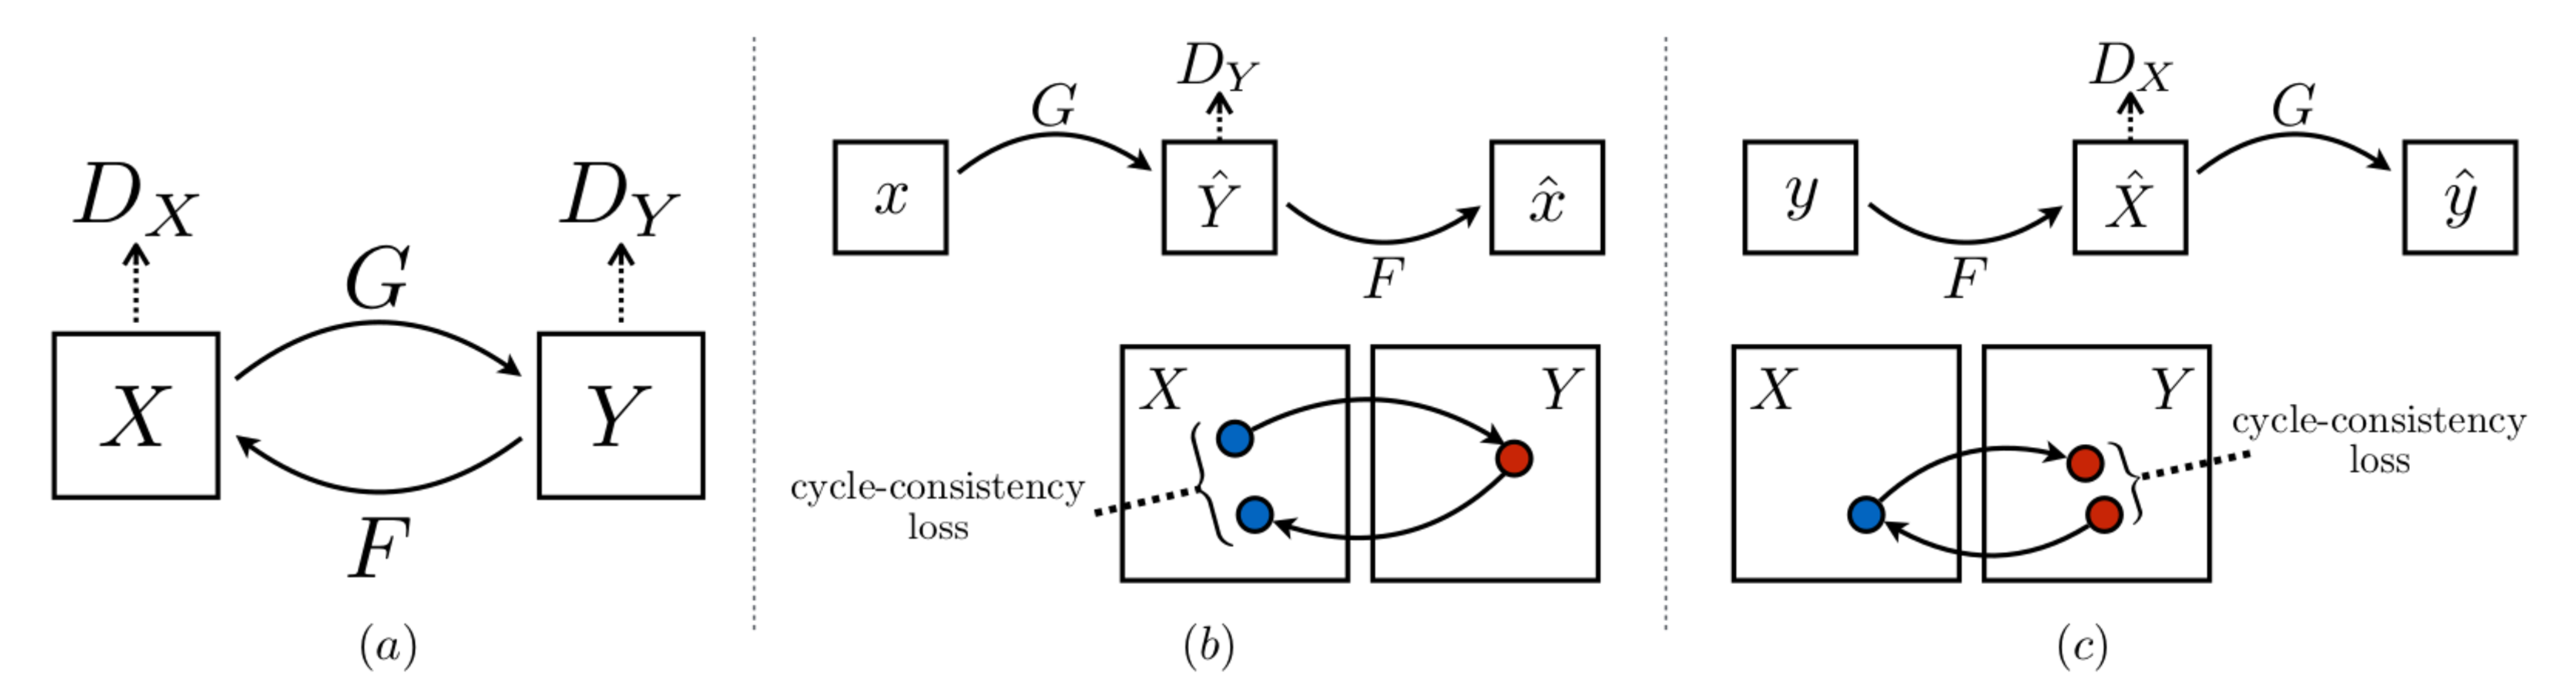
\includegraphics[width=\textwidth]{figures/cyclegan.pdf}
	\caption{CycleGAN训练示意图。图片来自文献~\cite{zhu2017unpaired}。}
	\label{fig:cyclegan}
\end{figure*}

CycleGAN~\cite{zhu2017unpaired}是一种新颖的非配对循环生成结构,主要思路是训练两对生成器和判别器模型将图像从一个域转换到另一个域,过程中要求循环一致性。实质上,CycleGAN在每个方向上都是单向GAN,共享两个生成器,各自带一个判别器,总共两个生成器两个判别器。网络结构如图~\ref{fig:cyclegan}所示,假设有$X$和$Y$两个域,生成器$G$基于$X$域图像生成$Y$域图像;生成器$F$基于$Y$域图像生成$X$域图像,这两个生成器是相反的过程,通过图~\ref{fig:cyclegan}(b)(c)中的循环一致性损失进行约束。CycleGAN的两个判别器$D_X$和$D_Y$分别用来判断输入$X$和$Y$域的图像真假。%因此,CycleGAN可以看作两个GAN的融合,一个GAN由生成器$G$和判别器$D_X$构成,实现从$X$到$Y$域图像的生成和判别;另一个GAN由生成器$F$和判别器$D_Y$构成,实现从$Y$域到$X$域的图像生成和判别,两个网络构成循环过程。
% \begin{equation}
% \label{equ:cyclegan}
% \begin{aligned}
% \mathcal{L}_{cyc}(F,G,X,Y) & = \mathbb{E}_{x \sim p_{data}(x)}[\parallel G(F(x))-x \parallel_1]\\
% & + \mathbb{E}_{y \sim p_{data}(y)}[\parallel G(F(y))-y \parallel_1]
% \end{aligned}
% \end{equation}
CycleGAN创新提出的循环一致性损失函数。
% 如~\ref{equ:cyclegan}所示,
映射$ G(F(y)) \approx y$和$ G(F(x)) \approx x$在训练过程中学习到。也就是$X$域图片翻译到$Y$域中,还能再逆转回来。%生成器$G$对应方向判别器$D_X$和生成器$F$对应方向判别器$D_Y$分别可以定义一个GAN对抗损失。%,最终目标函数~\ref{equ:cycle_obj}由两个方向上的对抗损失加上循环一致性损失三部分组成。    

% \begin{equation}
% \label{equ:cycle_obj}
% \begin{aligned}
% \mathcal{L}=\mathcal{L}_{GAN}(F,D_Y,X,Y)&+\mathcal{L}_{GAN}(G,D_X,X,Y)\\
% & + \lambda \mathcal{L}_{cyc}(F,G,X,Y)
% \end{aligned}
% \end{equation}


\subsubsection{图像多模态翻译}
从UNIT~\cite{liu2017unsupervised}以共享潜在空间为假设看成图像求联合概率分布,实现非配对的两个域之间分解表达的图像翻译。包括UNIT在内,当时图像翻译无论是配对还是非配对方法,大都是一对一,即输入一张图像只能生成一种风格,缺乏生成结果多样性。比如,同一个场景不同光照条件就是一个模式,不仅仅是白天和黑夜风格,也有傍晚、清晨等风格。在UNIT分解表达学习基础上,MUNIT和DRIT进一步提出多模态图像翻译方法。

MUNIT将潜在空间的潜在编码分为内容编码$c$和风格编码$s$。不同域的图像共享内容编码空间$C$而独享风格编码空间$S$。如图~\ref{fig:munit}(a)部分所示,域$X_1$的风格编码空间为$s_1$内容编码空间为$c_1$,域$X_2$的风格编码空间为$s_2$内容编码空间为$c_2$。内容控制图像中低维信息,风格描述图像中高维属性如颜色、纹理、样式等。网络架构清晰,两个编码器$E_1$ $E_2$分别生成域$X_1$和域$X_2$的内容编码和风格编码;两个生成器$G_1$ $G_2$分别生成域$X_1$和域$X_2$的图像结果;两个判别器$D_1$ $D_2$分别判别域$X_1$和域$X_2$的图像真假。

\begin{figure*}[ht]
    \centering
	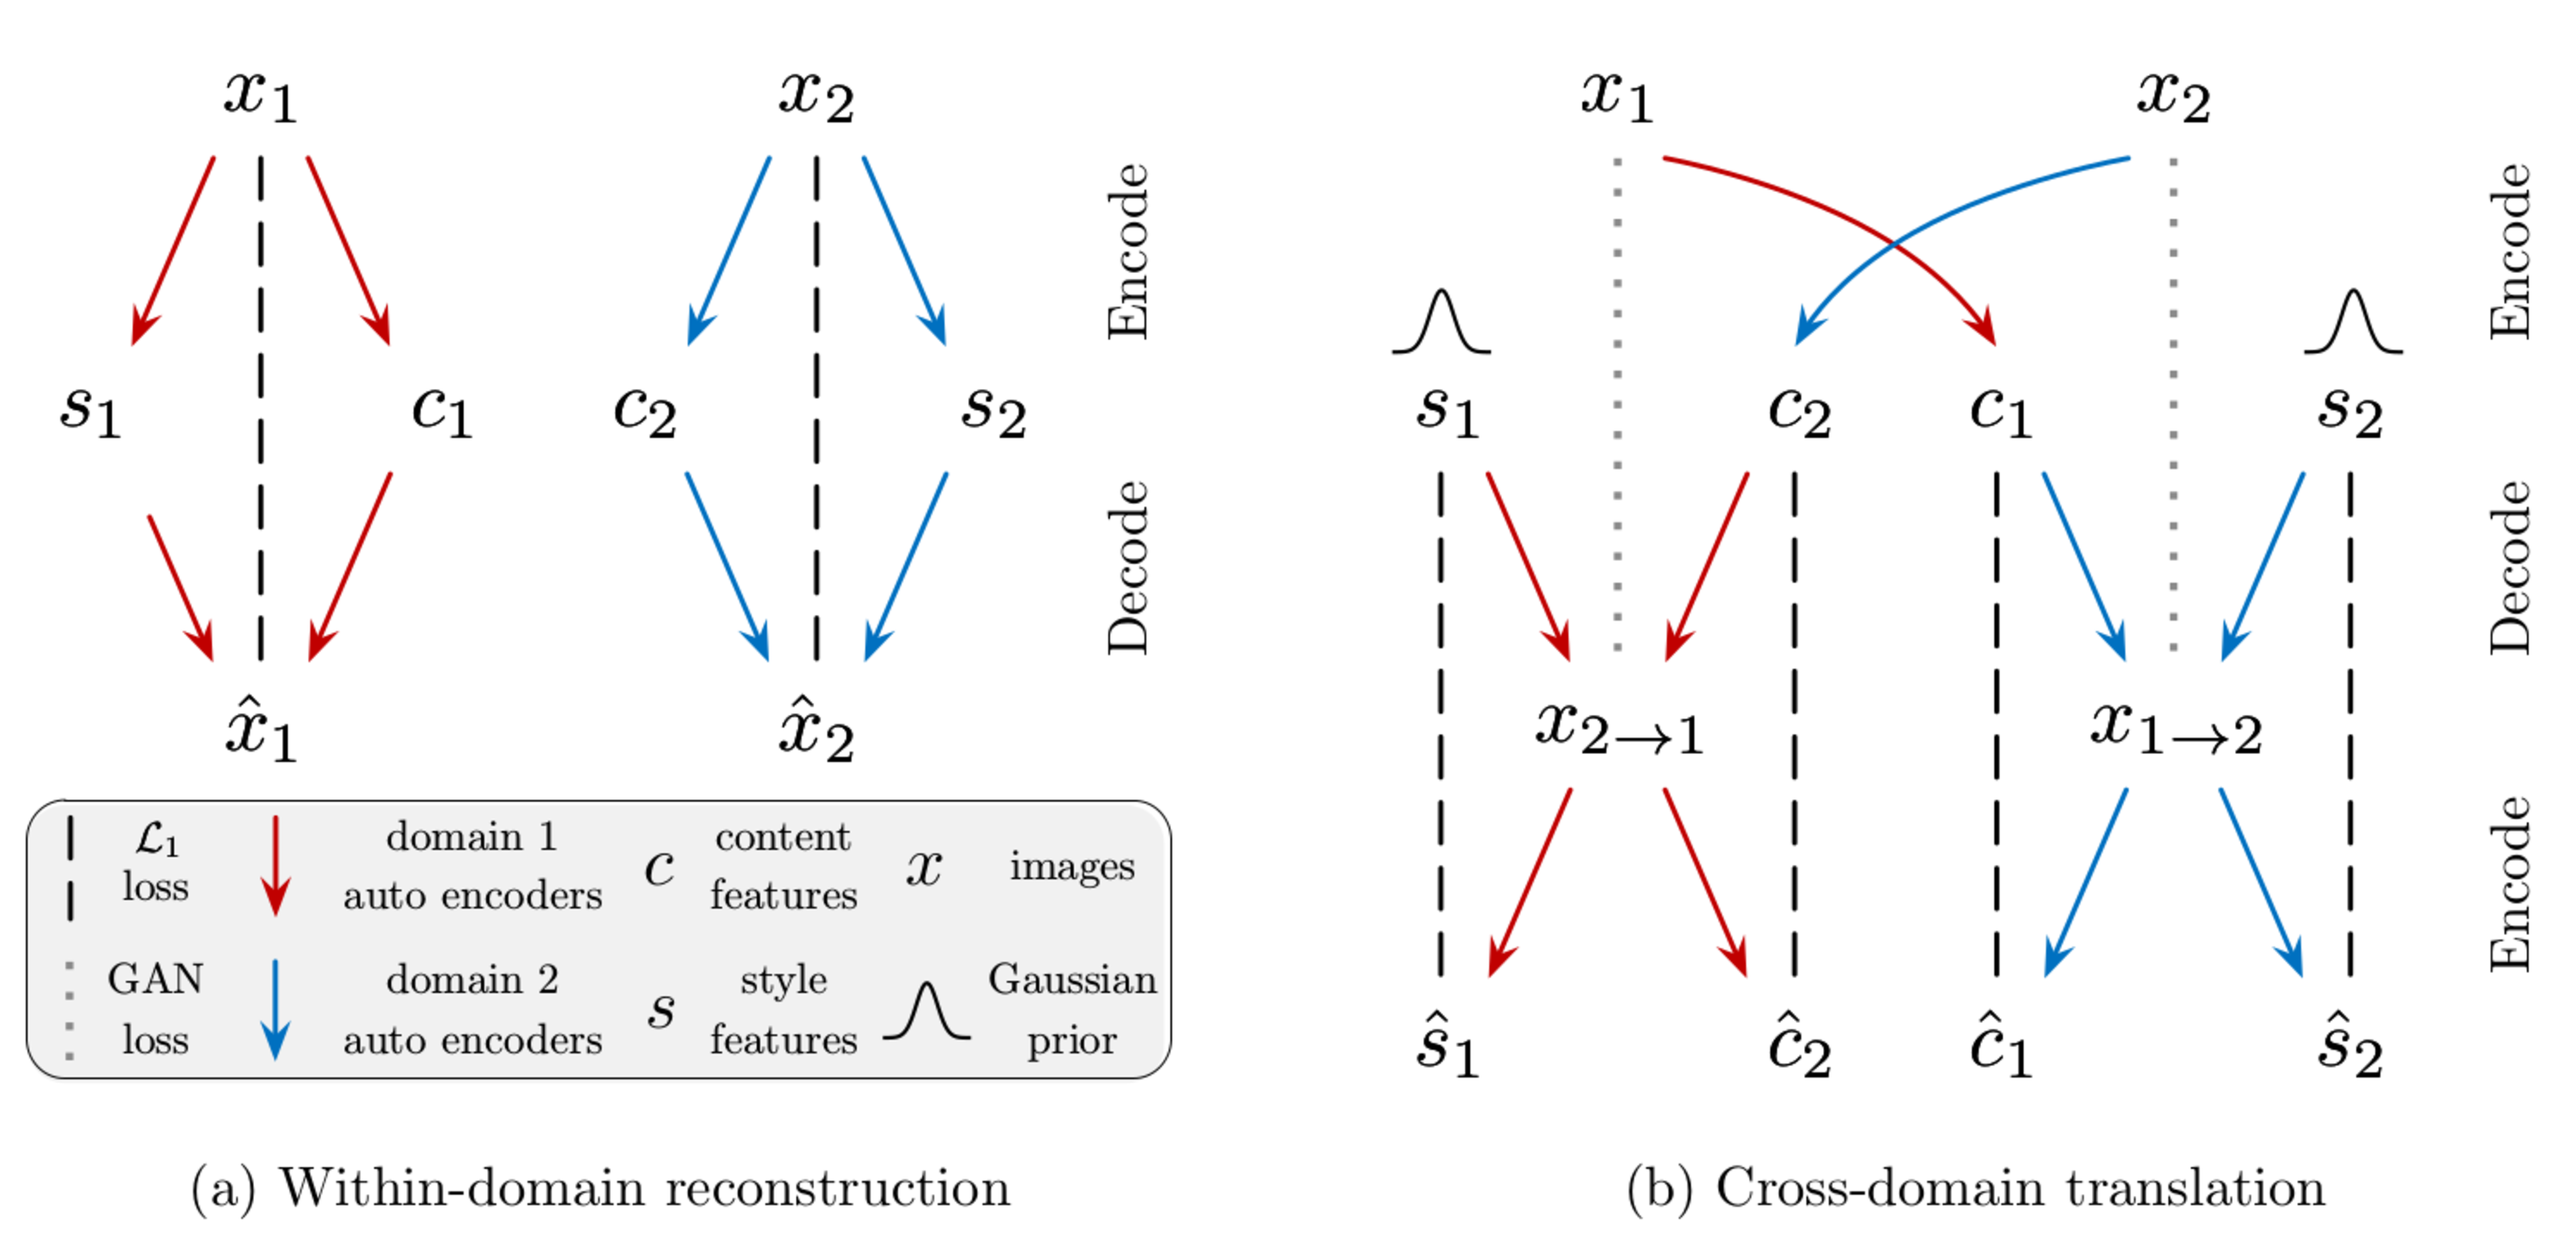
\includegraphics[width=\textwidth]{figures/munit.pdf}
	\caption{MUNIT训练示意图。图片来自文献~\cite{huang2018multimodal}。}
	\label{fig:munit}
\end{figure*}

整个网络的训练包括两个部分,如图~\ref{fig:munit}(a)所示的域内重建和如图~\ref{fig:munit}(b)所示的跨域翻译。
% 域内重建时,输入图像$x_1 \in X_1$经过编码器$E_1$可以得到内容编码$c_1$和风格编码$s_1$,即$c_1,s_1=E_1(x_1)$,再输入到域$X_1$的生成器$G_1$,形成图像$\hat{x_1}=G_1(c_1,s_1)$。
% 同样的,输入图像$x_2 \in X_2$经过编码器$E_2$可以得到内容编码$c_2$和风格编码$s_2$,即$c_2,s_2=E_2(x_2)$,再输入到域$X_2$的生成器$G_2$,形成图像$\hat{x_2}=G_2(c_2,s_2)$。
% 跨域翻译时,输入图像$x_1 \in X_1$经过编码器$E_1$可以得到内容编码$c_1$和风格编码$s_1$,即$c_1,s_1=E_1(x_1)$,保留内容编码$c_1$与满足正态分布的随机风格编码$s_2$同时输入到生成器$G_2$中,生成具有域$X_2$风格的图像$x_{1 \rightarrow 2}=G(c_1,s_2)$。
% ;同样的,输入图像$x_2 \in X_2$经过编码器$E_2$可以得到内容编码$c_2$和风格编码$s_2$,即$c_2,s_2=E_2(x_2)$,保留内容编码$c_2$与满足正态分布的随机风格编码$s_1$同时输入到生成器$G_1$中,生成具有域$X_1$风格的图像$x_{2 \rightarrow 1}=G(c_2,s_1)$。
MUNIT结构包括生成结构和判别结构,生成结构包括编码器和解码器。编码器包括内容编码器和风格编码器,解码器采用AdaIN~\cite{huang2017arbitrary}仿射变换将目标域风格翻译;判别器使用多尺度判别器~\cite{wang2018high}结构,能帮助实现高分辨率图像的判别。由此,可以构建重建损失函数包括图像重建损失函数,内容重建损失和风格重建损失函数。

% \begin{equation}
% % \label{equ:munit_rec_x1}
% \begin{split}
% \mathcal{L}_{recon}^{x_1} = \mathbb{E}_{x_1 \sim p(x_1)}[\parallel G_1(E_1^c(x_1),E_1^s(x_1))-x_1\parallel_1] \\
% \mathcal{L}_{recon}^{c_1} = \mathbb{E}_{c_1 \sim p(c_1), s_2 \sim q(s_2)}[\parallel E_2^c(G_2(c_1,s_2))-c_1\parallel_1] \\
% \mathcal{L}_{recon}^{s_2} = \mathbb{E}_{c_1 \sim p(c_1), s_2 \sim q(s_2)}[\parallel E_2^s(G_2(c_1,s_2))-s_2\parallel_1]
% \end{split}
% \label{munit}
% \end{equation}

% \begin{equation}
% \label{equ:munit_rec_x2}
% L_{recon}^{x_2} = \mathbb{E}_{x_2 \sim p(x_2)}[\parallel G_2(E_2^c(x_2),E_2^s(x_2))-x_2\parallel_1]
% \end{equation}

% 由此,可以构建重建损失函数包括图像重建损失函数(如式~\ref{equ:munit_rec_x1}),内容重建损失(如式~\ref{equ:munit_rec_c1})和风格重建损失函数(如式~\ref{equ:munit_rec_s2})。

% \begin{equation}
% \label{equ:munit_rec_c1}
% \mathcal{L}_{recon}^{c_1} = \mathbb{E}_{c_1 \sim p(c_1), s_2 \sim q(s_2)}[\parallel E_2^c(G_2(c_1,s_2))-c_1\parallel_1]
% \end{equation}

% \begin{equation}
% \label{equ:munit_rec_c2}
% L_{recon}^{c_2} = \mathbb{E}_{c_2 \sim p(c_2), s_1 \sim q(s_1)}[\parallel E_1^c(G_1(c_2,s_1))-c_2\parallel_1]
% \end{equation}

% \begin{equation}
% \label{equ:munit_rec_s1}
% L_{recon}^{s_1} = \mathbb{E}_{c_2 \sim p(c_2), s_1 \sim q(s_1)}[\parallel E_1^s(G_1(c_2,s_1))-s_1\parallel_1]
% \end{equation}

% \begin{equation}
% \label{equ:munit_rec_s2}
% \mathcal{L}_{recon}^{s_2} = \mathbb{E}_{c_1 \sim p(c_1), s_2 \sim q(s_2)}[\parallel E_2^s(G_2(c_1,s_2))-s_2\parallel_1]
% \end{equation}

% 目标函数(如式~\ref{equ:munit})是对抗损失(如式~\ref{equ:munit_adv})以及重建损失函数之和。
% \begin{equation}
% \label{equ:munit_adv}
% \begin{aligned}
% \mathcal{L}_{GAN}^{x_2} = & \mathbb{E}_{x_2 \sim p(x_2)}[\log D_2(x_2)] \\
% & +\mathbb{E}_{c_1 \sim p(c_1), s_2 \sim q(s_2)}[\log(1-D_2(G_2(c_1,s_2)))]
% \end{aligned}
% \end{equation}

% \begin{equation}
% \label{equ:munit}
% \begin{aligned}
% \min \limits_{E_1,E_2,G_1,G_2} \max \limits_{D_1,D_2} \mathcal{L}(E_1,E_2,G_1,G_2,D_1,D_2) & = \mathcal{L}_{GAN}^{x_1}+\mathcal{L}_{GAN}^{x_2} \\
% & +\lambda_x(\mathcal{L}_{recon}^{x_1}+\mathcal{L}_{recon}^{x_2}) \\
% & + \lambda_c(\mathcal{L}_{recon}^{c_1}+\mathcal{L}_{recon}^{c_2}) \\
% & +\lambda_s(\mathcal{L}_{recon}^{s_1}+\mathcal{L}_{recon}^{s_2})
% \end{aligned}
% \end{equation}


DRIT~\cite{lee2018diverse}跟MUNIT在思路上完全一致,都是共享内容空间,独享属性/风格空间。网络训练如图~\ref{fig:drit}所示同样由域内重建和跨域翻译两个部分组成,跨域翻译用来生成交换风格厚的图像,域内重建被编码后的潜在编码。用$X, Y$表示两个域,网络由两个内容编码器$E_{X}^{c}$和$E_{Y}^{c}$和两个属性编码器$E_{X}^{a}$和$E_{Y}^{a}$,两个生成器$G_X$和$G_Y$以及两个判别器$D_X$,$D_Y$组成。其中$u=G_X(E_Y^c(y),E_X^a(x))$,$v=G_Y(E_X^c(x),E_Y^a(y))$。

\begin{figure*}[ht]
    \centering
	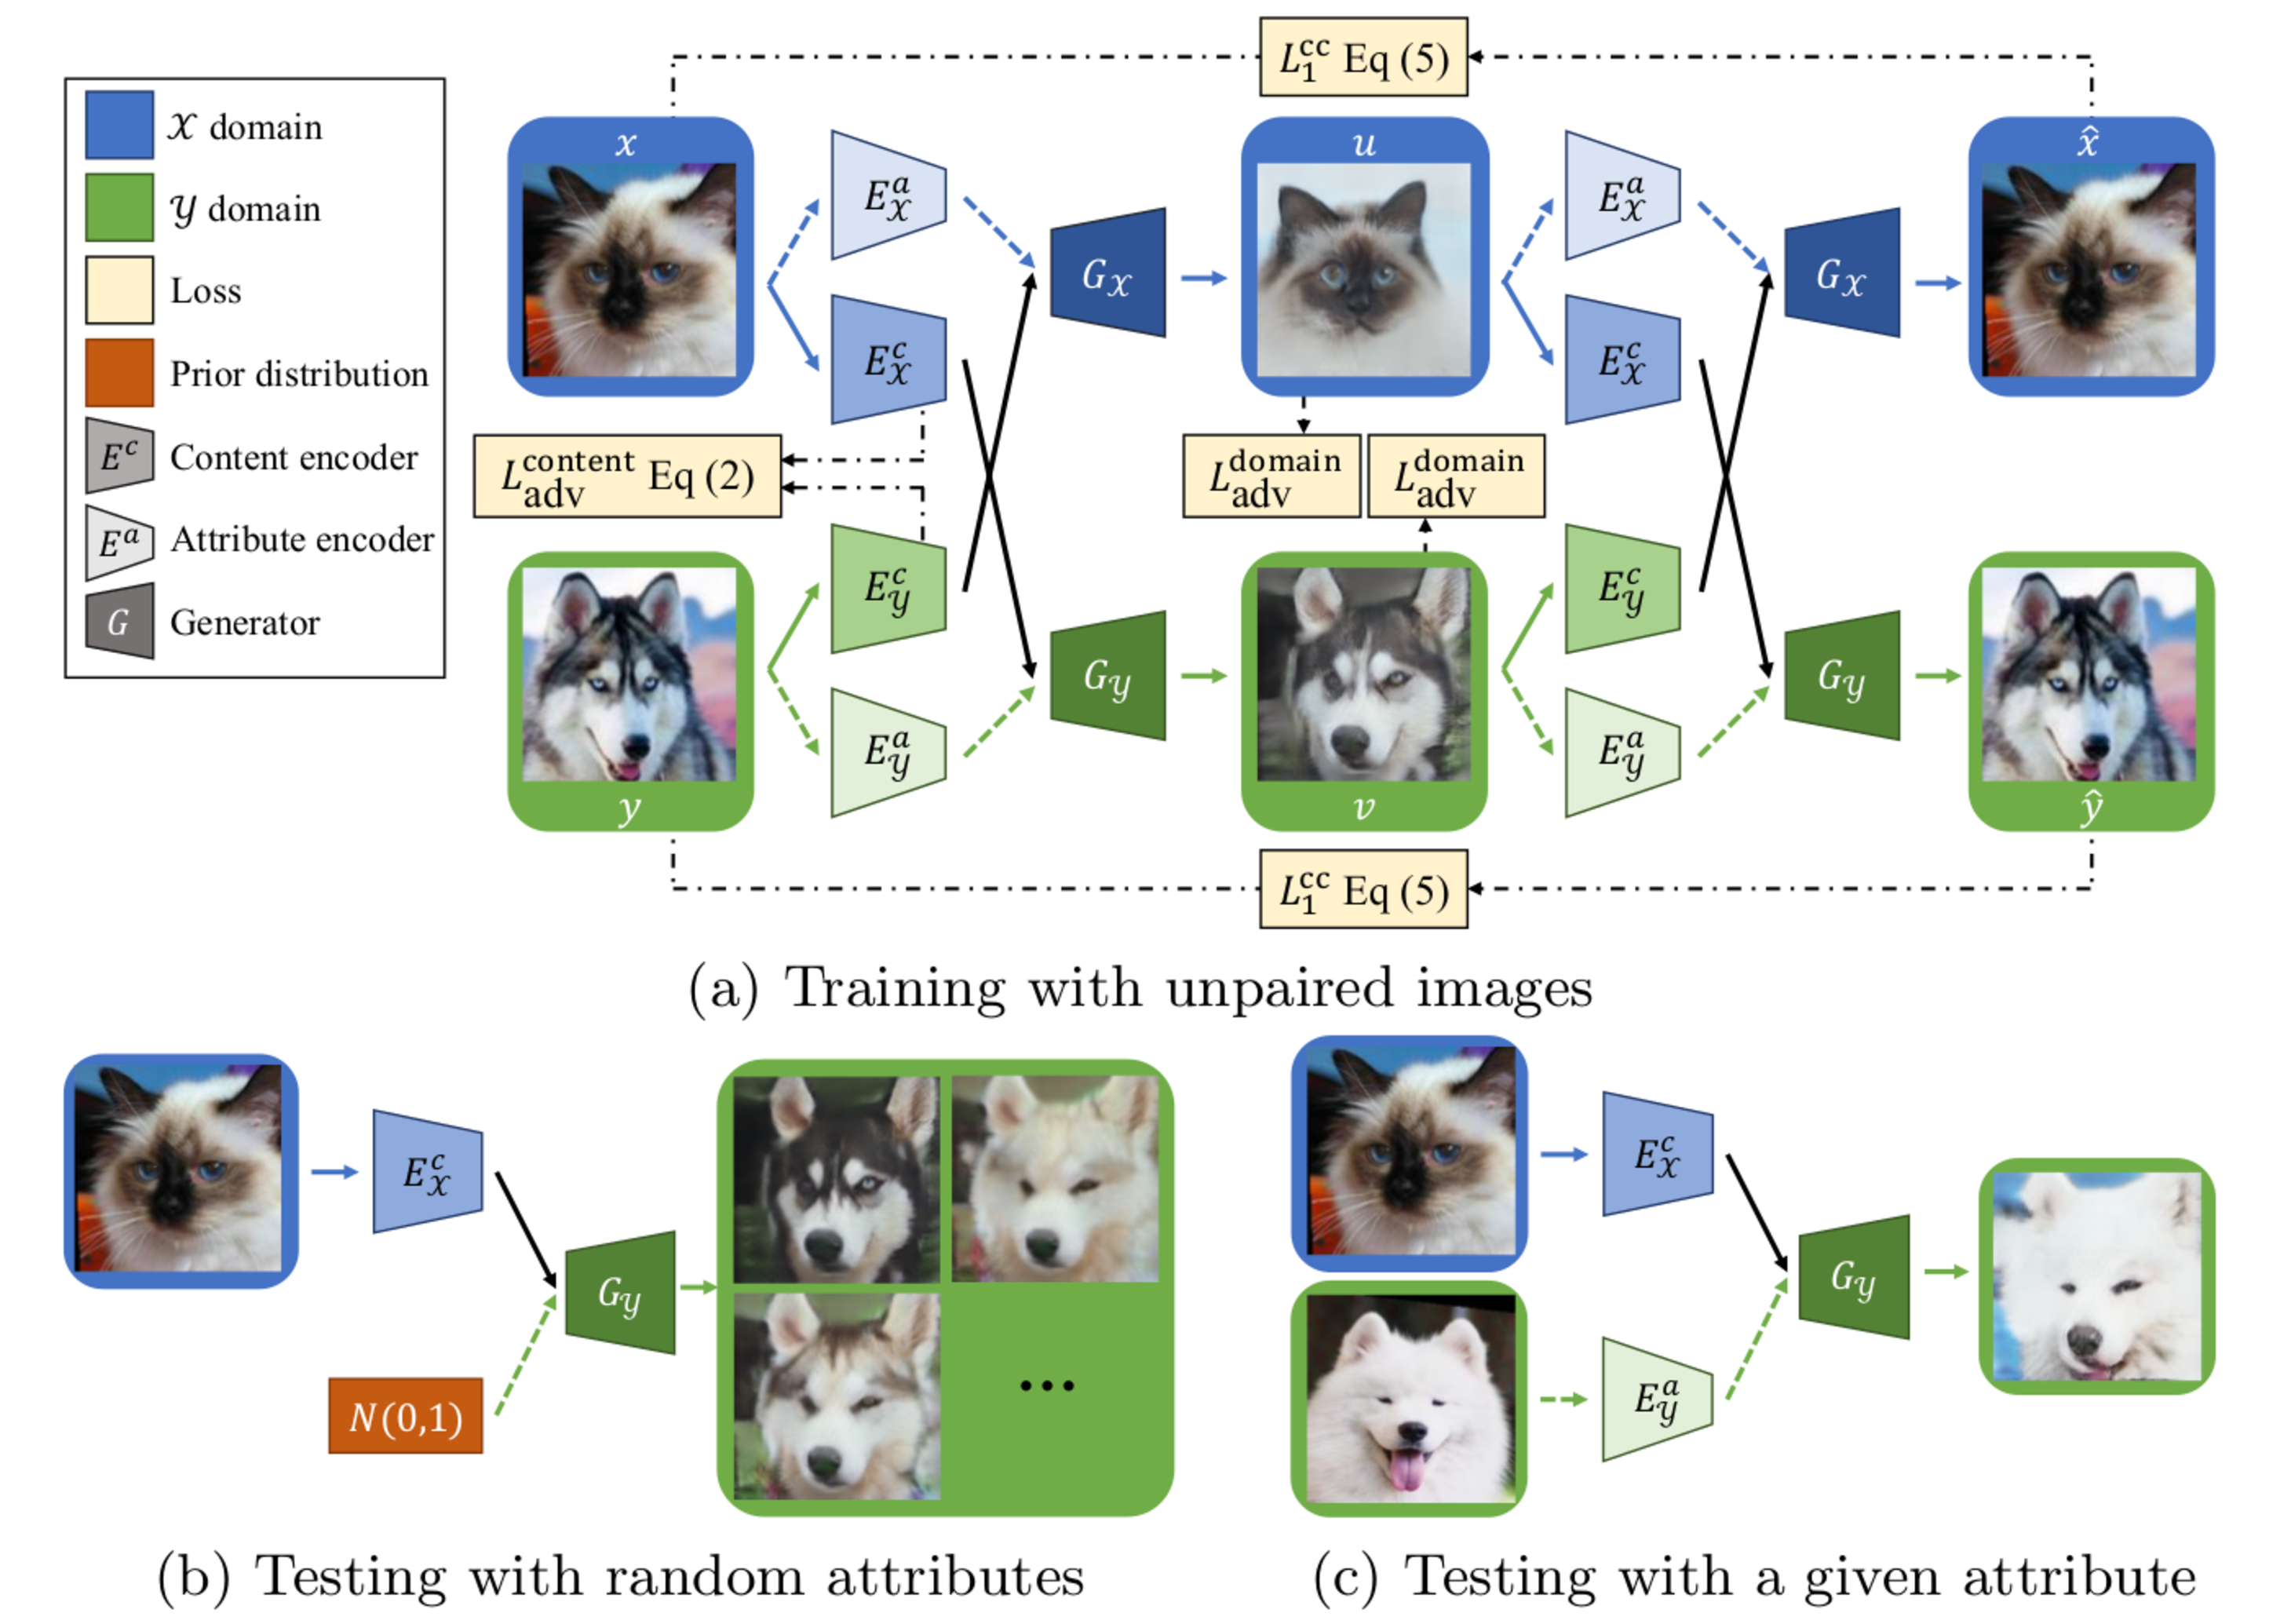
\includegraphics[width=\textwidth]{figures/DRIT.pdf}
	\caption{DRIT训练示意图。图像来自文献~\cite{lee2018diverse}。}
	\label{fig:drit}
\end{figure*}

跨域翻译和域内重建跟MUNIT一致,在此不再赘述。在内容编码和属性编码结合时,DRIT和MUNIT有一定的差异,MUNIT将风格编码使用AdaIN内嵌到生成器(解码器)的中间层,而DRIT采用共享两个编码器$E_X^c$,$E_Y^c$最后一层和两个生成器$G_X$,$G_Y$第一层的权值。
% 共享权值的情况下,为了区分两个域的编码文中提出使用判别损失~\ref{equ:drit_adv}。

% \begin{equation}
% \label{equ:drit_adv}
% \begin{aligned}
% \mathcal{L}_{adv}^{content} & = \mathbb{E}_x[\frac{1}{2}\log D^c(E_X^c(x))+\frac{1}{2}\log(1-D^c(E_X^c(x)))] \\
% & + \mathbb{E}_y[\frac{1}{2}\log D^c(E_Y^c(y))+\frac{1}{2}\log(1-D^c(E_Y^c(y)))] 
% \end{aligned}
% \end{equation}

% 损失函数中也加入CycleGAN中提出的循环一致性损失~\ref{equ:drit_cc},其中$u=G_X(E_Y^c(y),E_X^a(x))$,$v=G_Y(E_X^c(x),E_Y^a(y))$。%,还有重建损失,对抗损失等。总的目标函数如~\ref{equ:munit}所示。

% \begin{equation}
% \label{equ:drit_cc}
% \begin{aligned}
% \mathcal{L}_1^{cc}(G_x,G_Y,E_X^c,E_Y^c,E_X^a,E_Y^a) = \mathbb{E}_{x,y}&[\parallel G_X(E_Y^c(v),E_X^a(u))-x \parallel_1 \\
% & + \parallel G_Y(E_X^c(u),E_Y^a(v))-y \parallel_1]
% \end{aligned}
% \end{equation}

DSMAP~\cite{chang2020domain}基于MUNIT分解表达方式,将图像分解到内容空间和风格空间,但DSMAP认为MUNIT内容空间分解不彻底,DSMAP提出将共享内容空间的特征进行再映射到域特有的内容潜在空间中。经过再一次分解,此时将内容信息再一次净化,得到纯净的域特有内容信息,有助于后续跨域翻译和域内重建的进行。此方法搭建一个更好的图像的内容域和样式域沟通的桥梁,使得最终生成的图像能更好更真实的表达出来。

\begin{figure*}[ht]
    \centering
	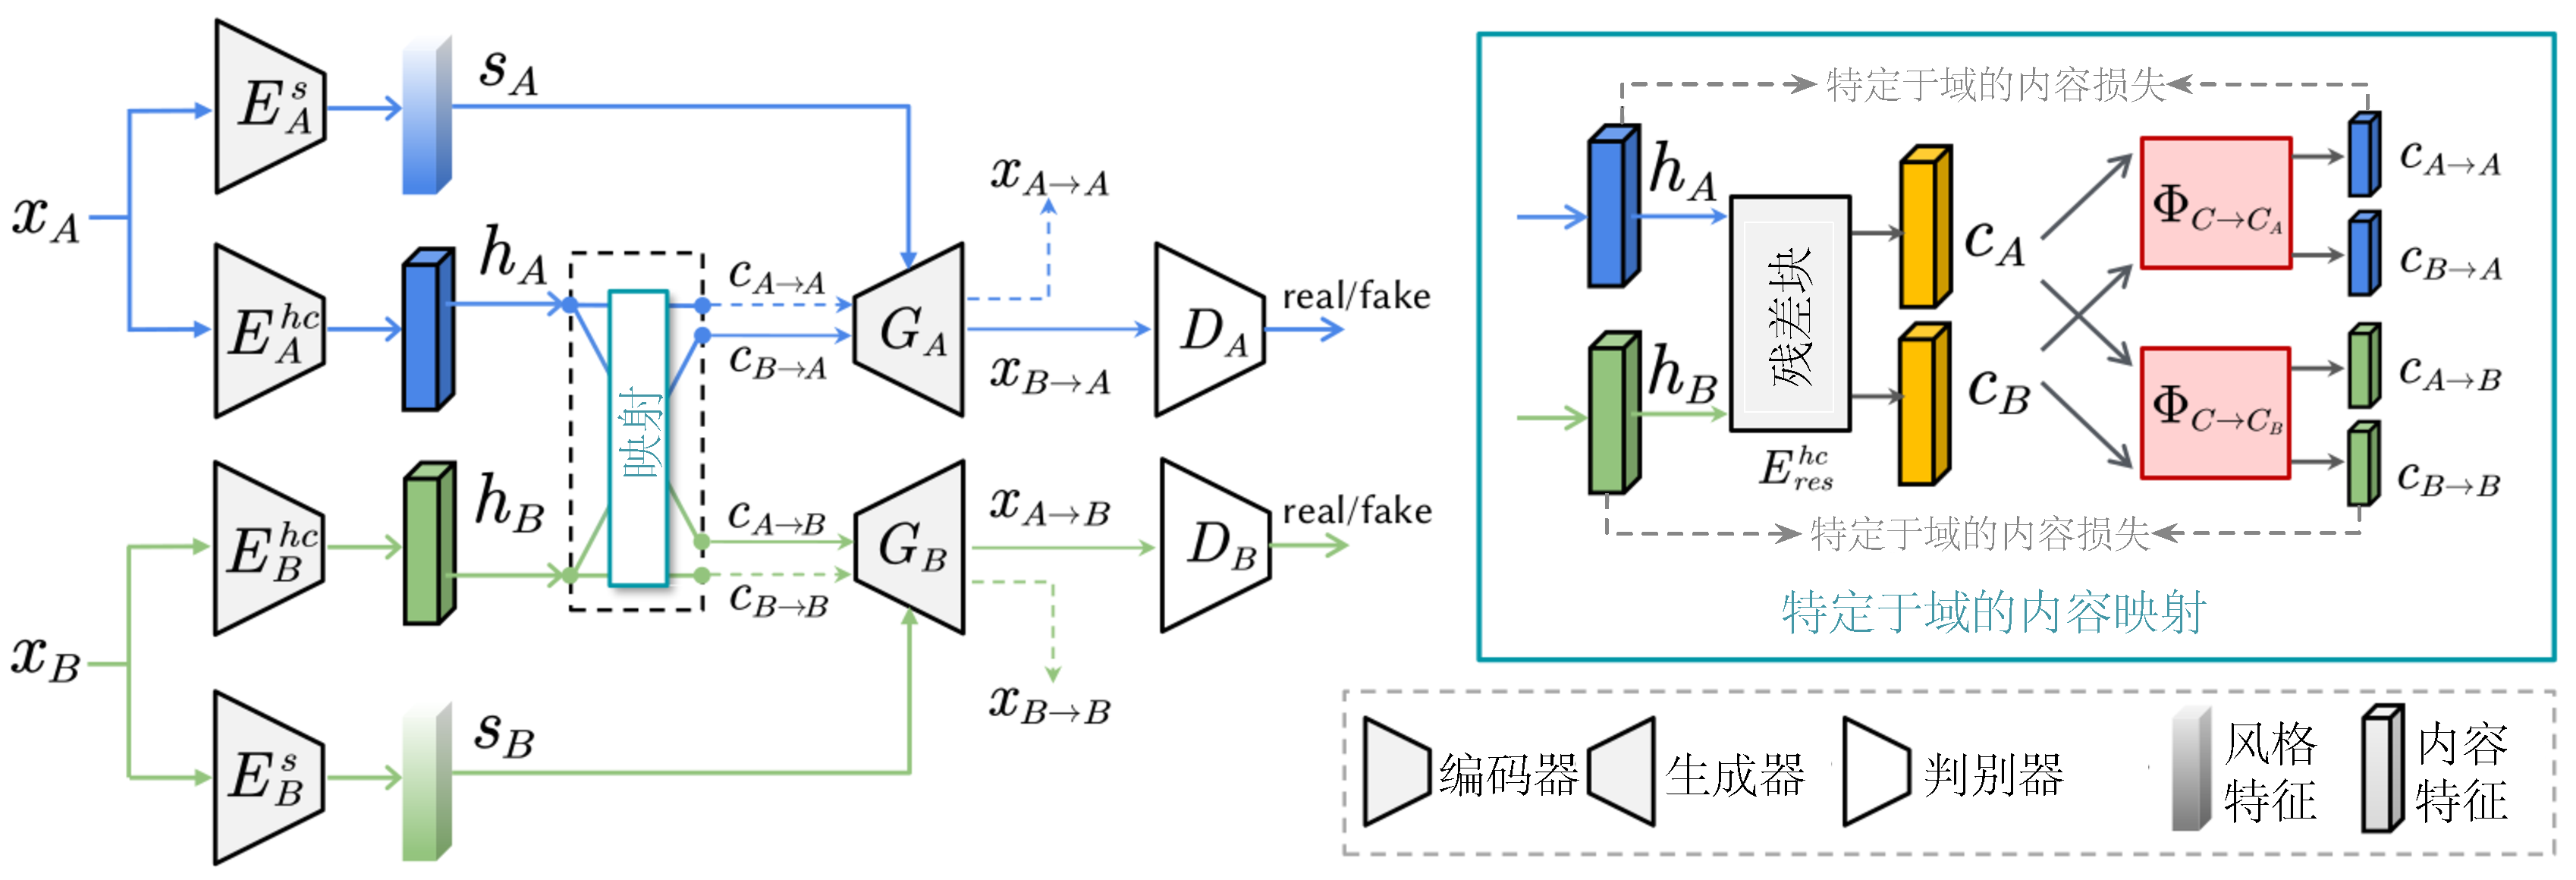
\includegraphics[width=\textwidth]{figures/DSMAP.pdf}
	\caption{DSMAP训练示意图。图像来自文献~\cite{chang2020domain}。}
	\label{fig:dsmap}
\end{figure*}

% \begin{equation}
% \label{equ:drit}
% \begin{aligned}
% \min \limits_{G,E,E^a} \max \limits_{D,D^c} & \lambda_{adv}^{content}\mathcal{L}_{adv}^c + \lambda_1^{cc}\mathcal{L}_1^{cc} + \lambda_{adv}^{domain}\mathcal{L}_{adv}^{domain} \\
% & + \lambda_1^{recon}\mathcal{L}_1^{recon} + \lambda_1^{latent}\mathcal{L}_1^{latent} + \lambda_{KL}\mathcal{L}_{KL}
% \end{aligned}
% \end{equation}

DRIT++~\cite{lee2020drit++}在DRIT基础上加入Mode Seeking Regulation~\cite{mao2019mode}解决模式崩溃问题并提高生成多模态样式的能力。StarGAN v2~\cite{choi2020stargan}引入映射网络和风格编码器将输入的风格噪声向量和输入风格图像编码到风格潜在空间,通过将随机采样的噪声向量输入生成目标域多模态结果。

\subsubsection{图像多域翻译}

\begin{figure*}[ht]
    \centering
	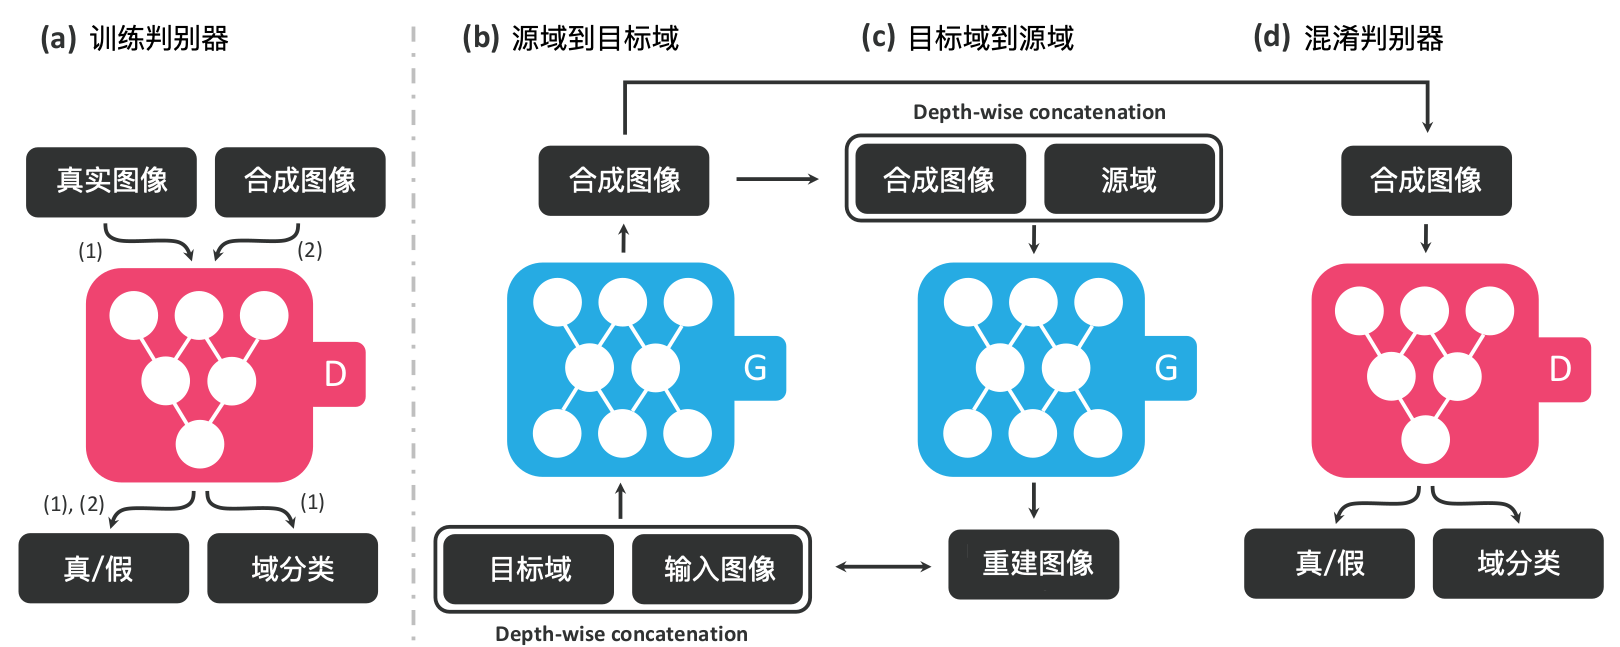
\includegraphics[width=\textwidth]{figures/star.png}
	\caption{StarGAN模型示意图。图像来自文献~\cite{choi2018stargan}。}
	\label{fig:star}
\end{figure*}

如图~\ref{fig:star}所示,StarGAN~\cite{choi2018stargan}将有同一种属性的一组数据作为一个域,对该属性进行属性编码,通过属性编码让生成器学会到多个域的翻译。在生成器的输入中添加目标域编码信息,判别器除了具有判断图片是否真实的功能外,还要有判断图片属于哪个域的能力。这样可以保证生成器中同样的输入图像,随着目标域的不同生成不同的效果。需要保证图像翻译过程中图像内容保存,只改变域间差异的那部分。StarGAN通过图像重建保证内容保持不变,图像重建即将图像翻译从域A到域B,再从域B到域A,此时重建结果与输入结果相比不会发生变化。StarGAN学习每个域的确定性映射,这可能无法获取数据分布的多模式性质。在给定源图像的情况下,它不可避免地在每个域中产生相同的输出。

\begin{figure*}[ht]
    \centering
	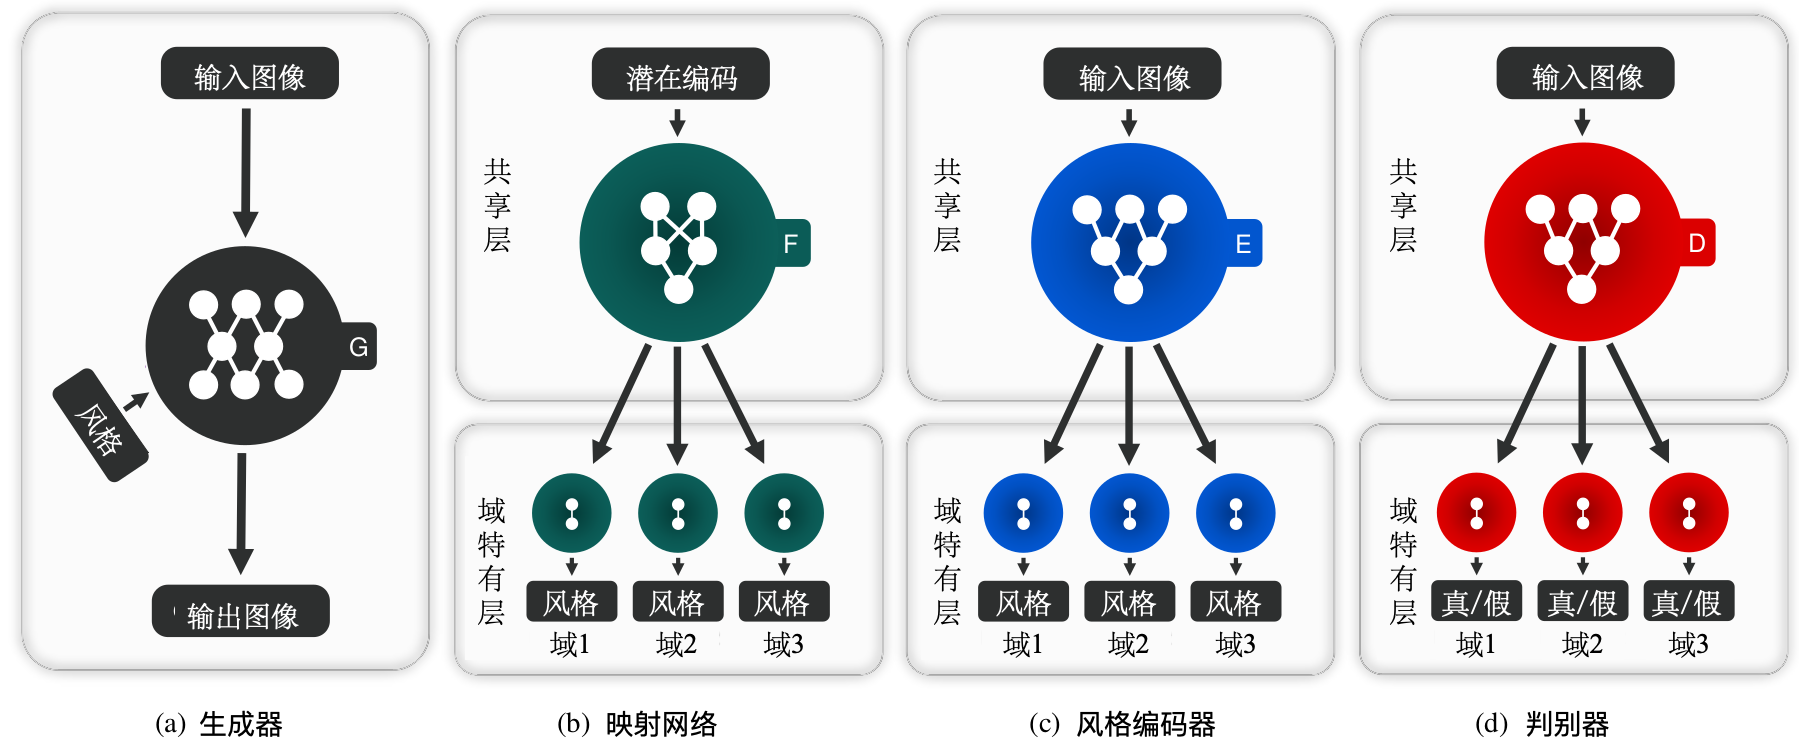
\includegraphics[width=\textwidth]{figures/starv2.png}
	\caption{StarGAN v2模型示意图。图像来自文献~\cite{choi2020stargan}。}
	\label{fig:starv2}
\end{figure*}

如图~\ref{fig:starv2}所示,StarGAN v2~\cite{choi2020stargan}以StarGAN为基础,用特定域的样式代码替换原来的域标签,这些代码可以表示特定域的各种形式。StarGAN v2引入两个模块,一个映射网络和一个样式编码器。前者学习将随机高斯噪声转换为样式代码,后者学习从给定的参考图像中提取样式代码。
StarGAN v2在图像质量、多样性和可扩展性方面与StarGAN和其它基准方法比实现了提升。

% \begin{figure*}[ht]
%     \centering
% 	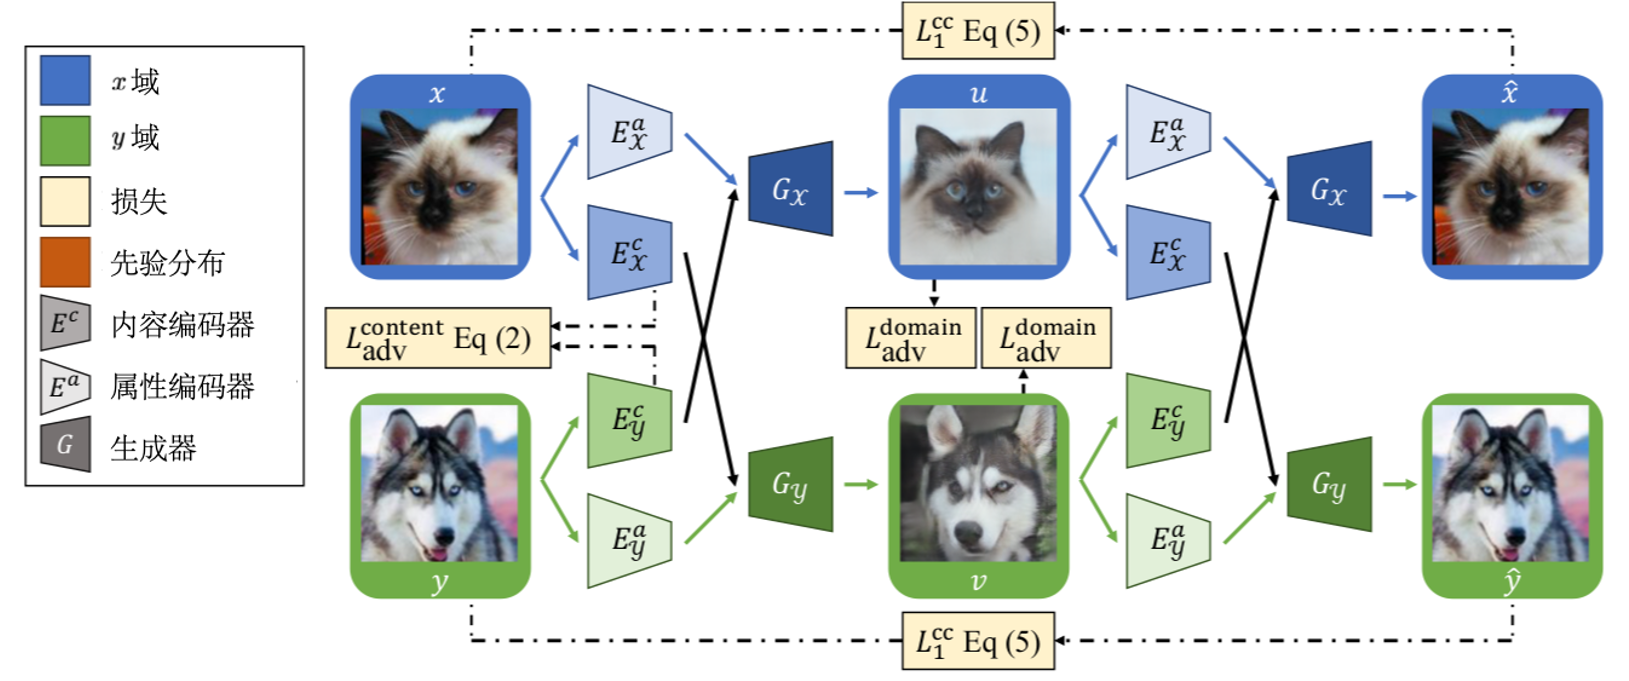
\includegraphics[width=\textwidth]{figures/DRIT++.png}
% 	\caption{DRIT++训练示意图。图像来自文献~\cite{lee2020drit++}。}
% 	\label{fig:drit++}
% \end{figure*}

DRIT++~\cite{lee2020drit++}则是在DRIT两个域多模态翻译任务基础上,通过分解表达用一个生成器进一步实现多域之间翻译。当为多个域的时候,输入其中两个域图像以及对应域内随机采样得到的one-hot编码,用DRIT中同样地的训练方法进行模型训练,将两个域之间的翻译拓展至多个域。

\section{水下图像翻译}\label{sec:underwater}
\subsection{水下图像成像}
水下环境的特殊物理和化学特性严重影响了水下图像的质量和数量,产生许多比在地面成像更难克服的问题。如图~\ref{fig:underwater}所示,水下成像有许多陆地图像不存在的问题。

\begin{figure*}[ht]
    \centering
	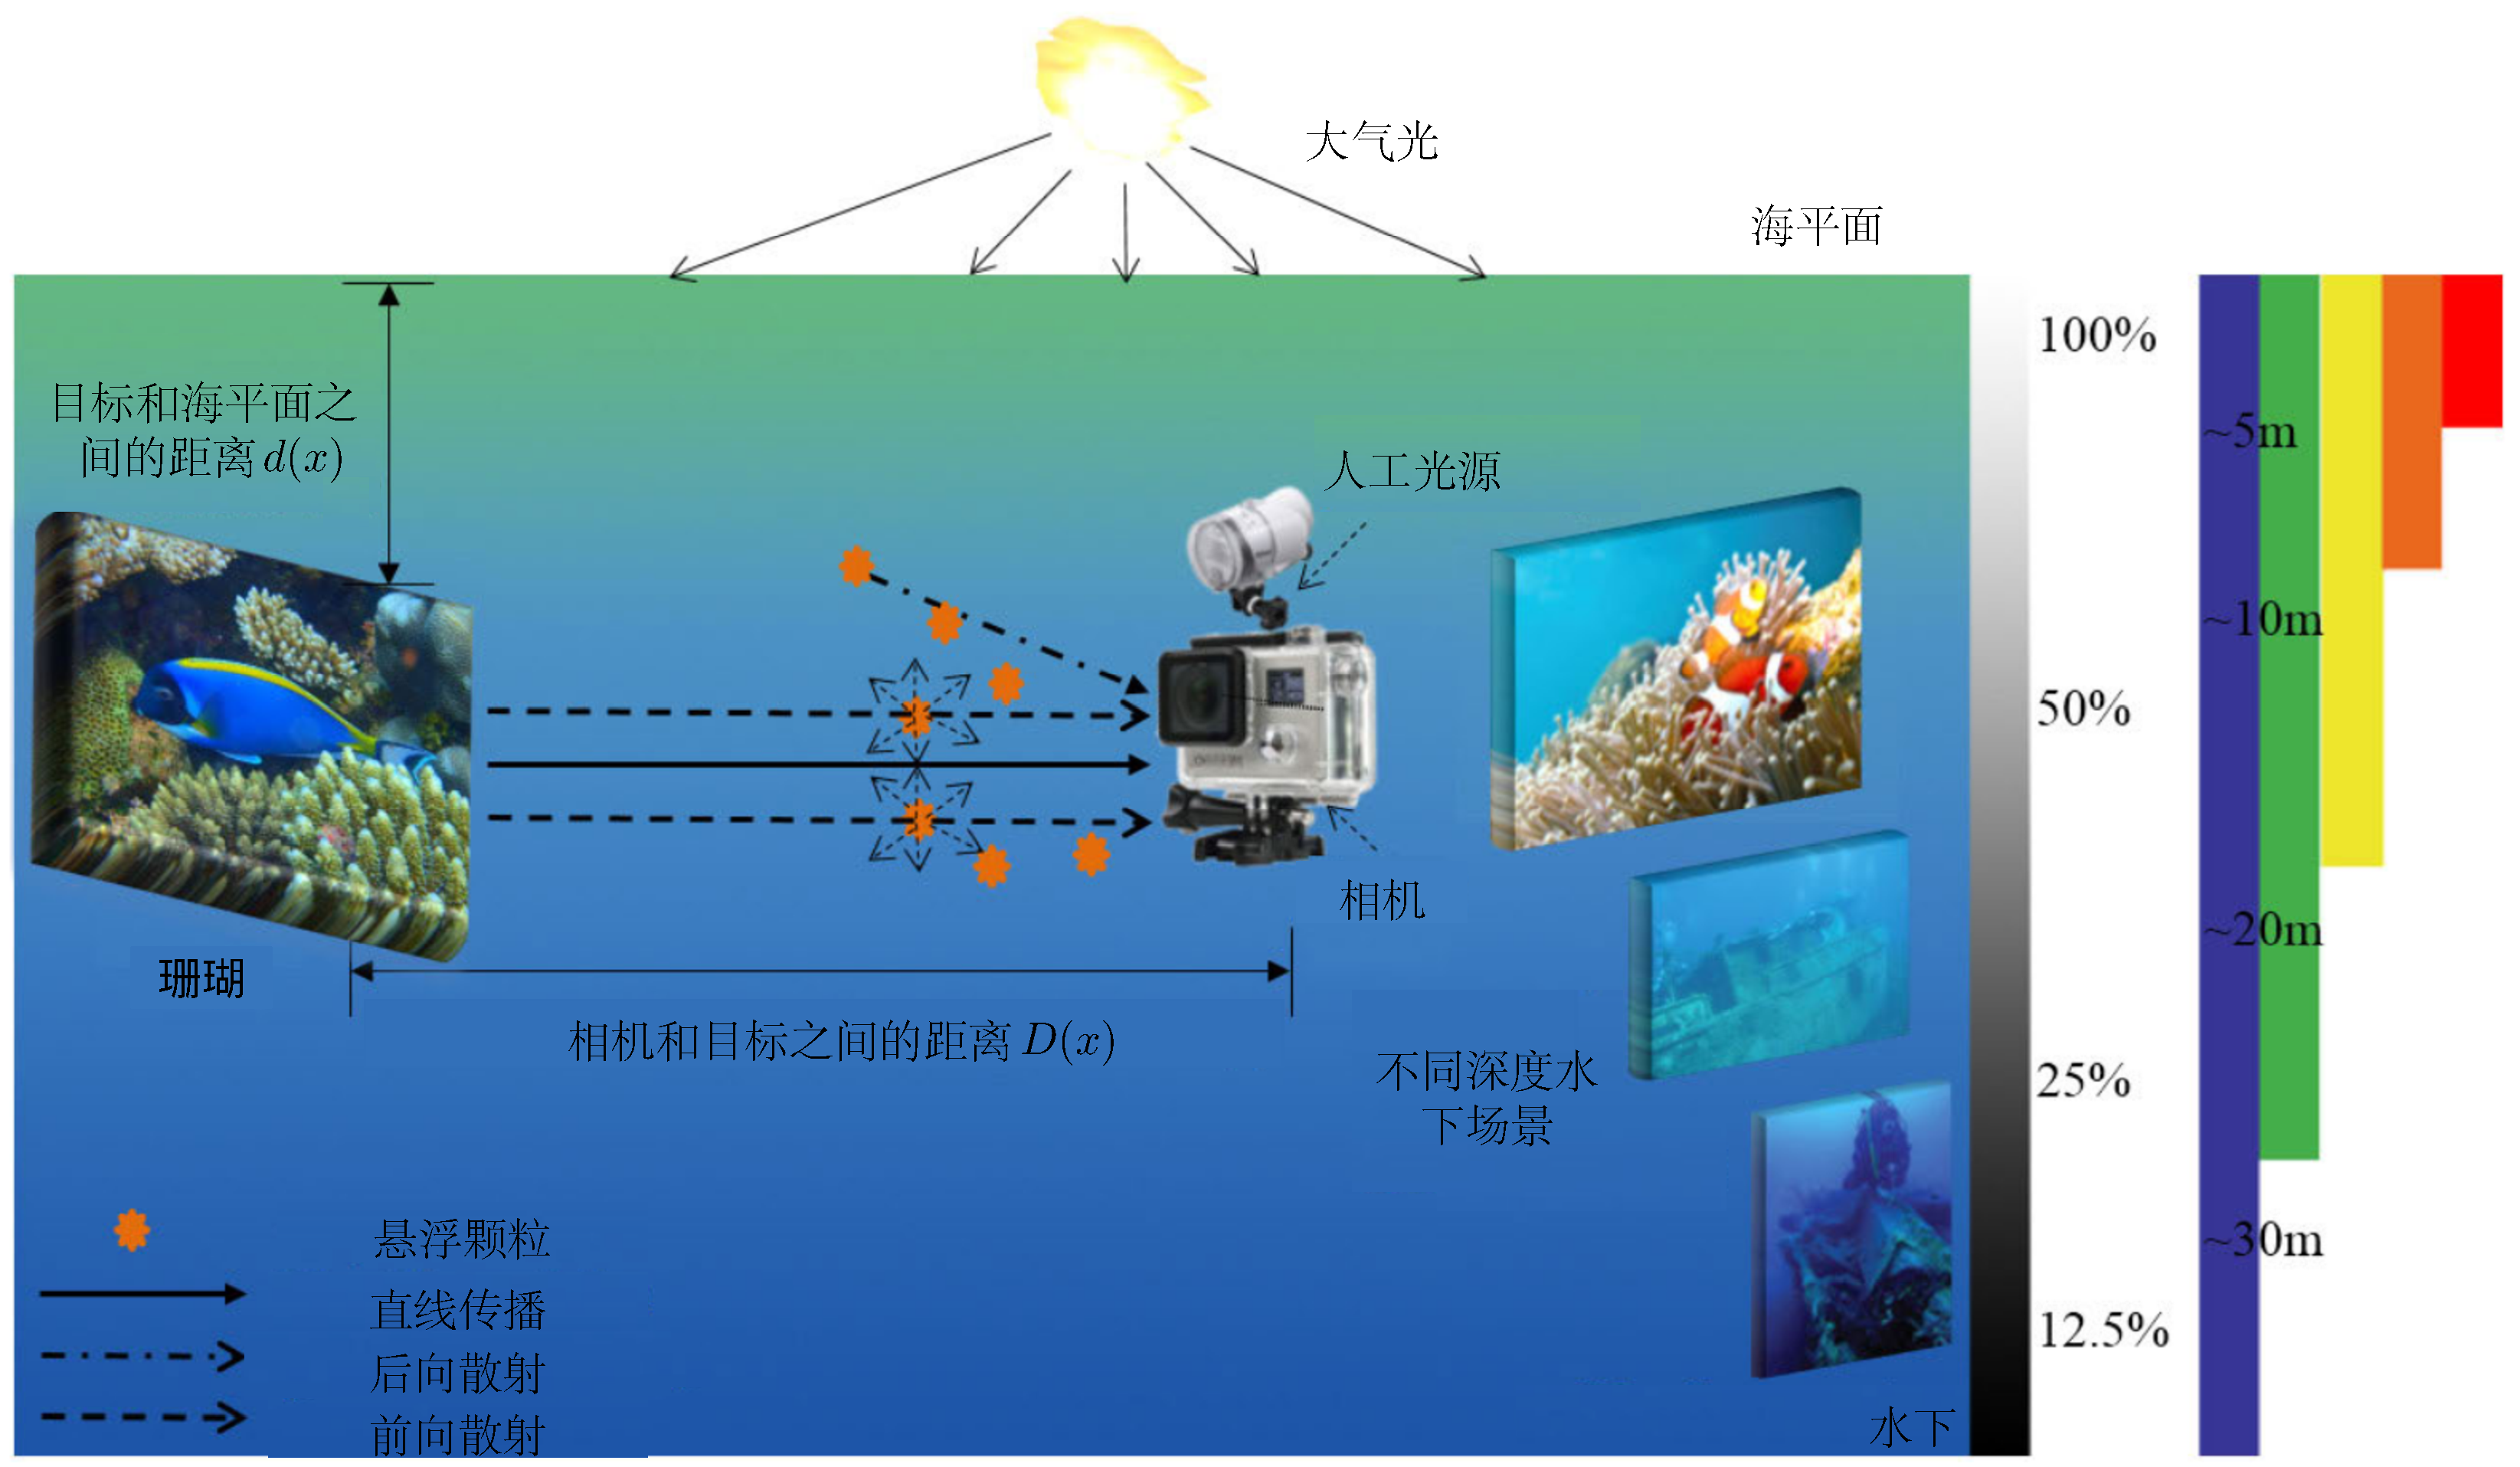
\includegraphics[width=\textwidth]{figures/水下成像.pdf}
	\caption{水下光学成像原理图。图片来自文献~\cite{2002Vision}。}
	\label{fig:underwater}
\end{figure*}

水下图像存在色偏的问题,图像视觉上会呈现蓝色、绿色和蓝绿色。这是由于不同颜色的光在水中的衰减特性造成的,红光波长较长,蓝色和绿色光波长较短,在水介质中光的传播过程中波长较长的光吸收速度更快,因此水下图像都是呈现蓝绿色调。

水下采集到的图像会存在对比度低,模糊等质量下降的问题。吸收和散射是图像降质的原因,即悬浮在水中的颗粒吸收了传播中的大部分光,并将水下场景的反射光在到达相机前改变了光的方向。人为光线除了吸收和散射,还会出现照明不均匀以及照明不足的问题,会造成阴影。

%水下成像公式

此外,由于水下环境的成像需要耗费巨大的人力和物力资源,水下图像数据量远远小于非水下自然场景的图像数据量,配对的多模态图像结果的获取更难能可贵。缺少水下图像数据给水下视觉研究造成巨大的困难,这也是研究人员针对水下视觉进行大量工作的原因。

\subsection{水下图像翻译}
目前现有的水下图像翻译有两种基本思路。一种是基于深度图和传输图等水下信息加入输入图像中或者基于水下成像衰减模型,使输入图像翻译成具有对应深度或者浑浊度的水下结果。另一种是基于非配对的图像翻译模型CycleGAN,两个域分别是空中图像域和水下图像域,通过循环一致性限制,学习从空中域图像到水下域图像的翻译。

%UWGAN

第一种思路有如下工作,每次生成水下图像类型固定,若要生成多样化结果需要训练多个模型依次对应。

WaterGAN~\cite{li2017watergan}用RGB-D~\cite{janoch2013category,lai2014unsupervised,silberman2011indoor,shotton2013scene}的地面图像数据集和水下图像样本集作为输入,使用WaterGAN翻译与RGB-D对齐的相应水下结果,获得成对的结果后在进行水下进一步水下研究。

Underwater-GAN~\cite{yu2018underwater}基于水下成像模型,使用浑浊度模拟器来模拟衰减的水下图像。生成数据集一般需要包括真实图像和对应深度图,在Underwater-GAN中设置相应的散射系数作为深度信息,根据模型计算出散射系数来翻译相对应的水下图像。

UIE-DAL~\cite{uplavikar2019all}和UWCNN~\cite{li2020underwater}使用NYU v2~\cite{silberman2012indoor}数据集中传输图作为衰减系数模拟近海岸和海洋里面不同水类型,控制衰减系数来进行10种水类型的图像翻译。这些方法生成的结果需要依赖于水下信息或者水下,对于真实水下采集到的图像数据缺少泛化能力。

第二种思路有如下工作,使用不成对的数据即可进行水下图像翻译,用非配对图像翻译模型CycleGAN只能实现一对一映射,翻译结果是单模态,缺乏多样性。同样地,要获得多种样式的结果需要多次实现。

UGAN~
\cite{fabbri2018enhancing}此类利用CycleGAN这个非配对一对一映射的图像翻译方法,一个域是空中图像、另一个域是水下图像,通过循环一致来学习从空中到水下图像的翻译。

MLFCGAN~\cite{liu2019mlfCGAN}和Jamadandi等人~\cite{jamadandi2019exemplar}提出的方法等都是用这种方法进行了水下图像翻译,不依赖于任何水下光学模型和任何物理信息。FUnIE-GAN~\cite{islam2020fast}通过相同的方法拓展成包括配对和不配对子集的大规模EUVP数据集。

我们希望通过一个网络模型,仅给定不配对的水下图像数据进行训练,就可以将给定图像同时翻译多种样式的水下结果。为了解决这个问题,可以借鉴我们研究的基于生成对抗网络的非配对图像域翻译的方法,根据水下图像的特点,重新设计相应有效的翻译模型,从而实现将给定图像到多样式水下图像的翻译。这样就可以实现从输入到输出一对多的映射,从而避免需要额外的信息而对数据有较高的要求并限制住模型的泛化能力。

\section{本章小结}
本章深入分析介绍了基于生成对抗网络的图像翻译方法,其中包括如下三个小节。

第一节介绍了生成对抗网络,引入生成对抗网络结构、原理以及目标函数,后续展示了生成对抗网络的发展过程中具有代表性的变种工作。

第二节介绍了基于生成对抗网络的图像翻译,详细讨论了成对图像翻译和非成对图像翻译经典模型,主要是广泛应用的非成对图像翻译基础上的多模态翻译和多域翻译的前沿工作。

第三节介绍了水下图像翻译,首先研究了水下图像的物理模型和成像特点,后分析了水下图像翻译的各种方法,对方法中存在的问题进行了详细的研究和讨论。
\chapter{水下图像合成研究}
海洋包含着未知的生物和巨大能源,对地球上生命延续起着重要的作用。自二十世纪中叶以来,高科技海洋勘测一直备受瞩目,视觉技术因能传达高密度信息而被应用在海洋环境中。研究人员致力于为水下机器人、水下救援、生态检测、海洋生物跟踪和实时导航等各种水下应用捕获高质量的水下图像。水下图像合成为水下应用的图像缺乏问题提供了一种行之有效的解决方式。

\section{水下图像成像原理及存在问题}
水下环境的特殊物理和化学特性严重影响了水下图像的质量和数量,产生许多比在地面成像的更难克服的问题。如图~\ref{fig:underwater}所示,水下成像存在的问题可以进行详尽分析。

\begin{figure*}[ht]
    \centering
	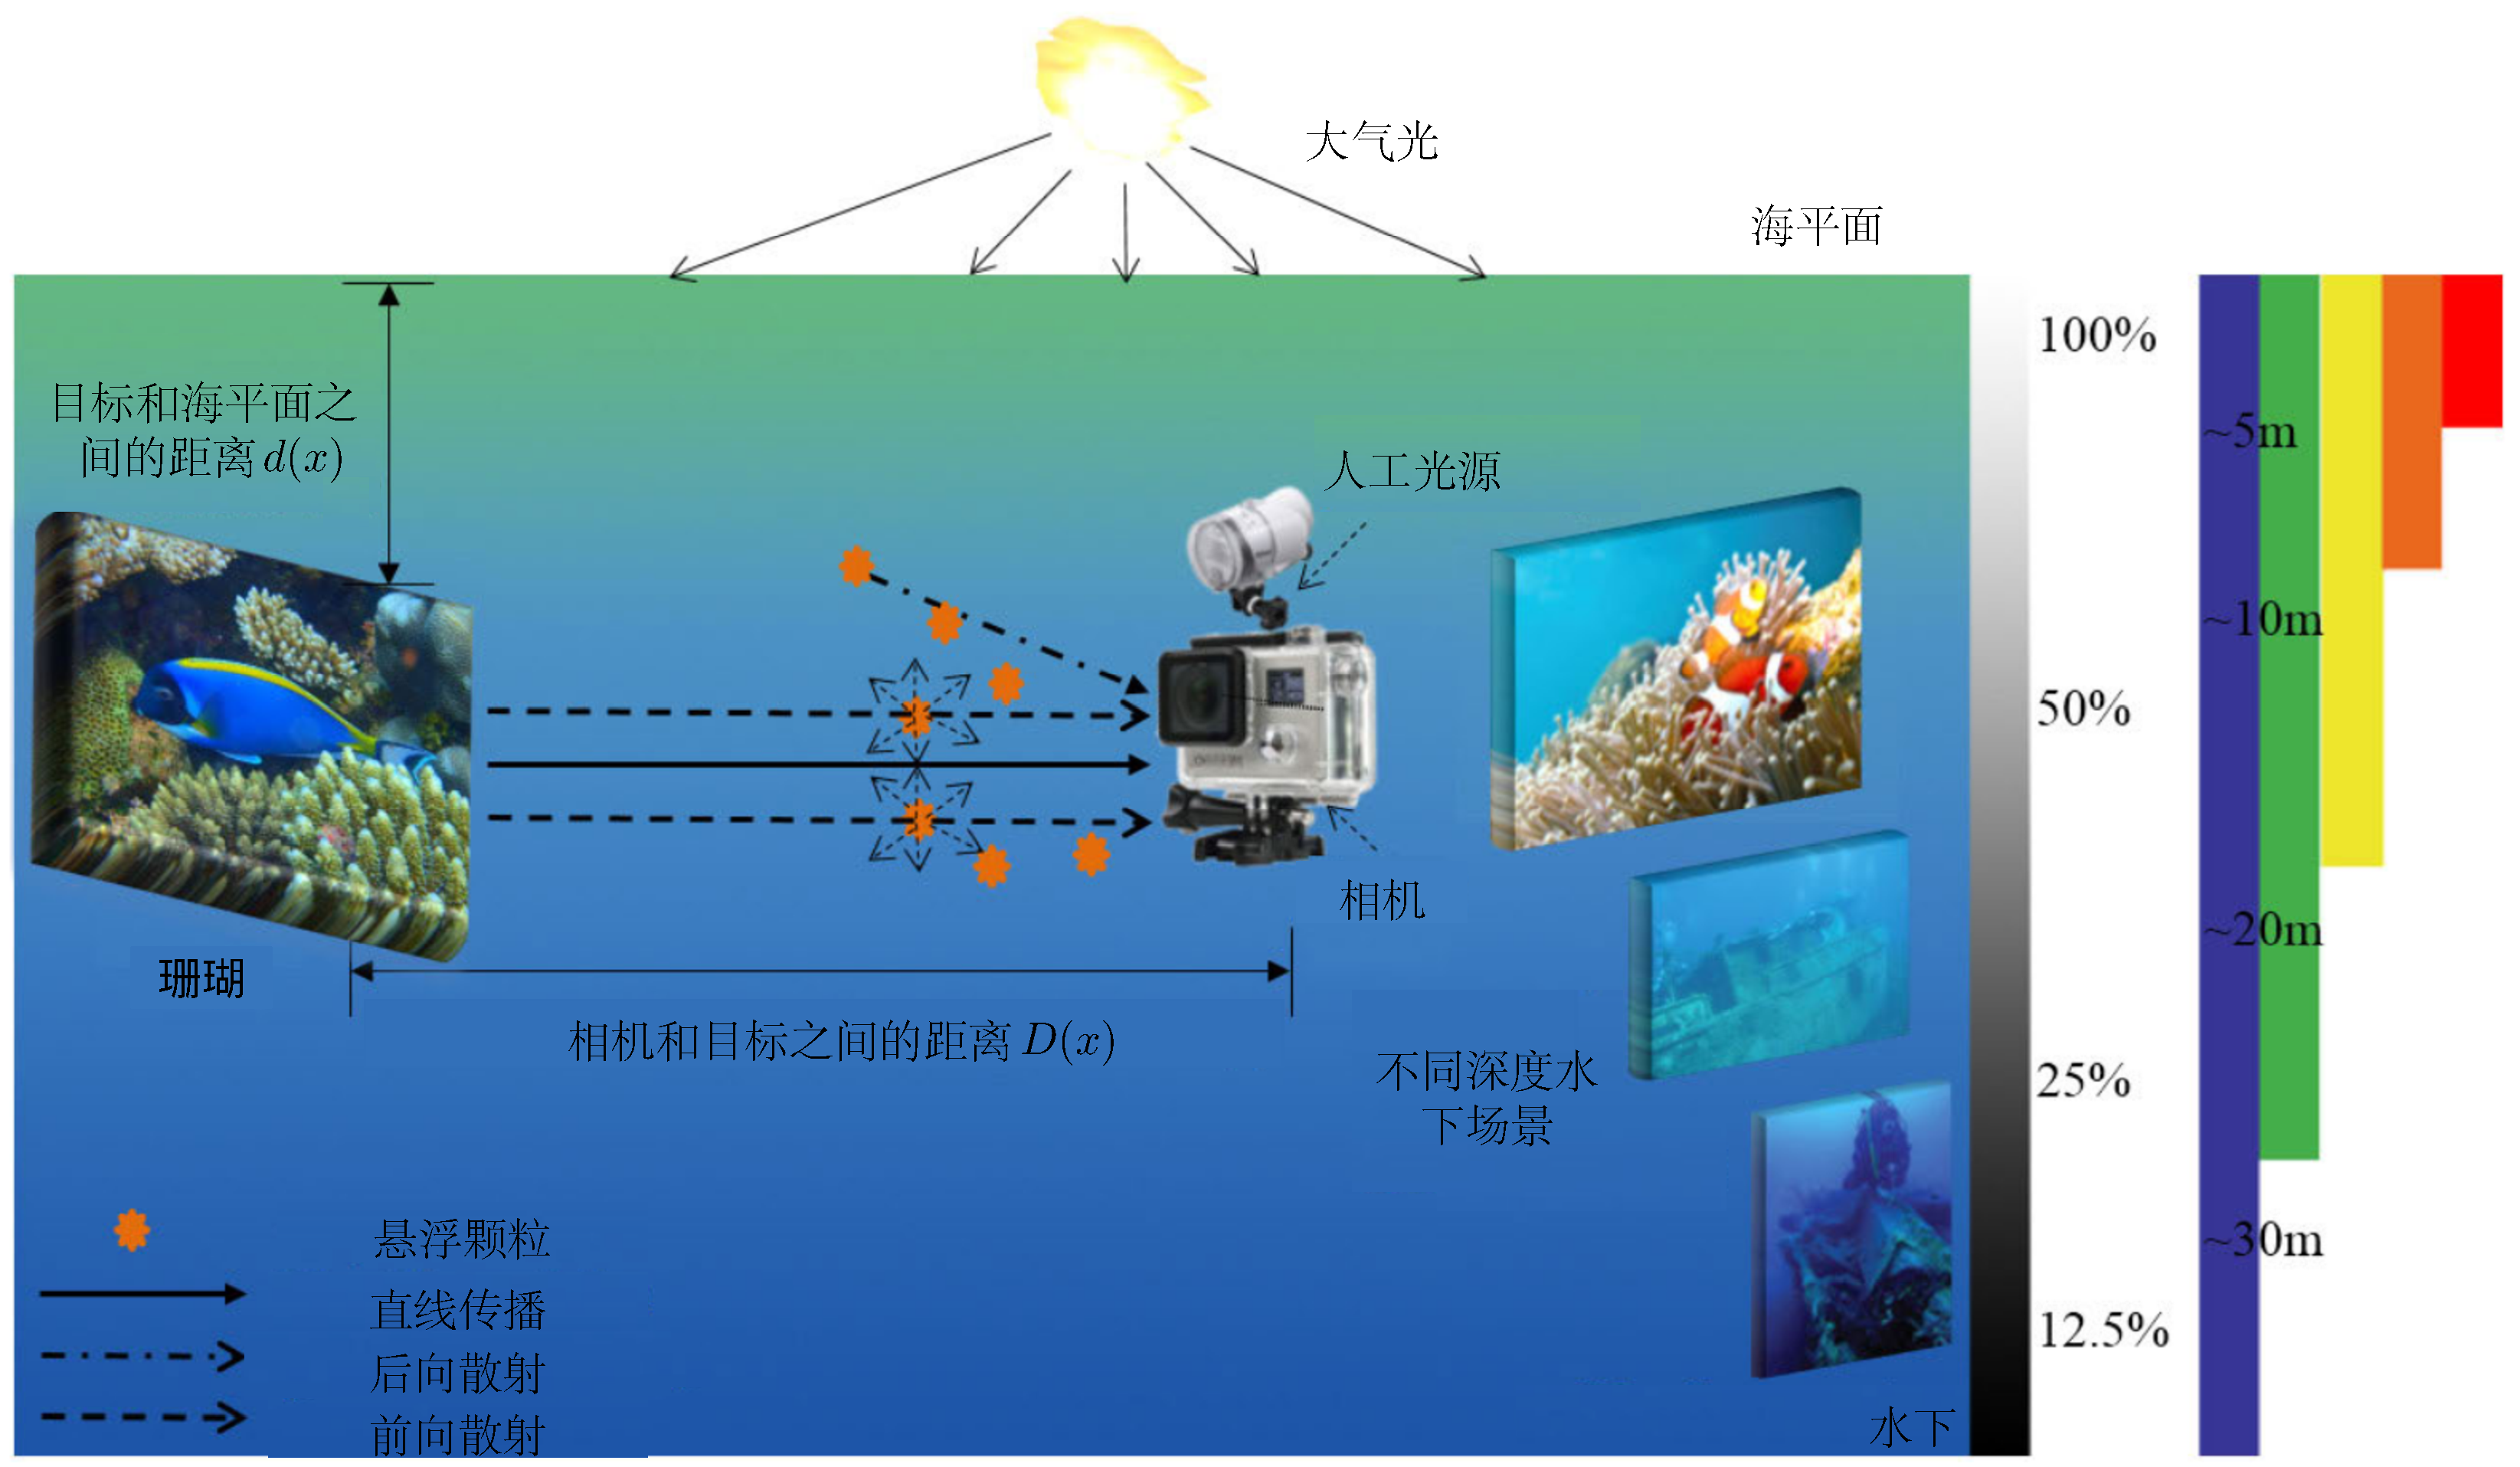
\includegraphics[width=\textwidth]{figures/水下成像.pdf}
	\caption{水下光学成像原理图。}
	\label{fig:underwater}
\end{figure*}

水下图像存在色偏的问题,图像视觉上会呈现蓝色、绿色和蓝绿色。这是由于不同颜色的光在水中的衰减特性造成的,红光波长较长,蓝色和绿色光波长较短,在水介质中光的传播过程中波长较长的光吸收速度更快,因此水下图像都是呈现蓝绿色调。

水下采集到的图像会存在对比度低,模糊的问题。吸收和散射,即悬浮在水中的颗粒吸收了传播中的大部分光,并将水下场景的反射光在到达相机前改变了光的方向,水的浑浊严重降低了图像质量。人为光线除了吸收和散射,还会出现照明不均匀以及照明不足的问题,会造成阴影。

%水下成像公式

此外,由于水下环境的成像需要耗费巨大的人力和物力资源,水下图像数据量远远小于非水下自然场景的图像数据量,配对的多模态图像结果的获取更难能可贵。缺少水下图像数据给水下视觉研究造成巨大的困难,这也是研究人员针对水下视觉进行大量工作的原因。

\section{水下图像合成研究}
\subsection{水下图像数据集}
由于真实水下场景的配对数据集数量有限,在水下视觉工作中也常用合成水下数据集进行研究。常用的真实数据集和合成水下数据集有如下几种,在我们实验中,根据实验设计将数据集组合进行使用,以达到训练目的。

RUIE~\cite{liu2019real}是共四千多的大规模真实水下数据集。针对可见度增强的性能进行评估的水下图像质量子集,包含五种质量的水下图像其中每种726张,用来测试水下图像增强效果;评估在不同照明和色偏算法的子集,包含蓝色、绿色以及蓝绿色三种色偏的水下图像每种100张;对高级计算机视觉任务如分类和检测的子集,包含对扇贝、海参和海胆三种海洋生物的标注每种100张。

UIEB~\cite{li2019underwater}是具有多样性场景、数量大以及具有高质量参考图像的成对真实场景数据集。原始图像图像共有950张,具有参考图像配对结果的890张,其余60张没有对应的参考图像。采用12种图像增强方法来进行图像增强,针对每张原始图像50个志愿者来选出令人满意的图像增强结果作为真值,令半数以上人不满意的60结果作为挑战图像没有真值。

像以上这种水下图像数据集相比较于非水下场景(空中)图像数量非常少,进行水下视觉图像研究时,研究人员会按照任务需要将空中图像进行水下环境条件模拟,合成该输入对应环境下的水下图像。

UWCNN~\cite{li2020underwater}论文中提出的从地面图像得到相应水下图像数据集。通过RGB-D NYU-v2~\cite{Silberman:ECCV12}室内数据集生成10种类型的水下图像。RGB-D NYU-v2室内共1449张图像,其中的1000张用于训练,剩下的449张用于测试,数据集提供的10类水图像也是共1449张图像。对于每张室内图像,根据生成的随机均匀全球大气光和深度(从0.5米到15米,每张图像生成5张水下图像。RGB-D NYU-v2室内数据集中的图像作为ground truth(真图),和合成的水下图像(假图)配对。

EUVP是UGAN~\cite{fabbri2018enhancing}中提出数据集的基础上更加齐全的数据集。UGAN中,ground truth是真实的相对不失真的水下图像(真图),配对的是生成的失真的水下图像(假图)。从ImageNet中选择一些不失真的水下图像,组成X域,共6143张图像,再从ImageNet中选择一些有明显水下图像特点的水下图像,组成Y域,共1817张图像。用CycleGAN实现风格迁移,即将X域中不失真的图像转成Y域中失真水下图像的风格(主要是颜色的变化)。最终用于训练的图像对是将X域中的图像都转译成失真水下图像。EUVP中,分为paired和unpaired两种。Paired文件夹中包含3个子文件夹:Underwater Dark、Underwater ImageNet和Underwater Scenes,其中Underwater Dark有5550个图像对,570张验证图像,共11670张;Underwater ImageNet有3700个图像对,1270个验证图像,共8670张图像;Underwater Scenes有2185个图像对,130个验证图像,共4500张图像。Unpaired:poor quality中有3195张,good quality中有3140张,validation中有330张,共6665张图像。

UVB 2017是一个模拟图像和视频数据集,是我们实验室在大连用ZED和Kinect摄像机进行拍摄的。用不同\ce{Al(OH)3}的浓度来模拟不同水质类型的衰减系数,摄像机收集了目标物在不同水质下的各种结果。已整理好的数据文件包括衰减为0即无水环境下的采集结果、衰减为1.2、1.58至衰减系数为3的多种结果。数据集在浑浊程度上随着衰减系数增加有视觉可见的从清晰到浑浊的变化过程。

\subsection{水下图像评价指标}
UCIQE~\cite{yang2015underwater}和UIQM~\cite{panetta2015human}是无参考/无真值评价水下图像质量的常用指标,是评价水下图像质量的关键指标。

UCIQM是色彩浓度,饱和度和对比度为测量分量的线性组合,可以定量的评价水下增强结果的色偏、模糊和对比度情况。属于无参考/无真值的图像质量评价指标,首先将水下图像从RGB颜色空间转换到CIELab颜色空间,这样更符合人类视觉感知,然后计算个测量分量,具体计算如式~\ref{equ:uciqe}所示。

\begin{equation}
\label{equ:uciqe}
UCIQE = c_1 \times \sigma_c + c_2 \times con_l + c_3 \times \mu_s
\end{equation}

其中,$ \sigma_c$为色度的标准方差,$con_l$为亮度的对比度,$\mu_s$是饱和度的平均值,$c_1$,$c_2$和$c_3$分别为线性组合的权重值。

UIQM针对水下图像的退化机理和成像特点,采用色彩测量UICM,清晰度测量UISM和对比度测量UIConM作为评价水下图像质量的依据。UIQM属于无参考/无真值的图像评价指标,通过测量分量的线性组合来表征图像的视觉质量,如式~\ref{equ:uiqm}所示。

\begin{equation}
\label{equ:uiqm}
UIQM = c_1 \times UICM + c_2 \times UISM + c_3 \times UIConM
\end{equation}

其中,$c_1$,$c_2$和$c_3$分别为线性组合的权重值,权重值的设定需要视具体任务而定,评价水下图像的颜色偏差修正结果时,需设定色度测量分量UICM更大的权重因子;当评价对比度和清晰度时,需要设定清晰度测量分量UISM和对比度测量分量UIConM更大的权重因子。

尽管,两种无参考的指标一定程度上给出定量的图像评价分数,但缺点也很明显。首先,水下图像质量不佳的视觉类型较多,仅参考几个测量分量的线性组合对于图像评价是片面的,缺少客观性和准确性;其次,测量分量权重的设置具有主观性,难以公正的评价水下图像质量;最后,评价结果域视觉效果不一致,会出现指标指示评价较好但视觉上没有直观的展现图像的优越性。


\subsection{经典水下图像合成方法}
目前现有的水下图像合成,目前有两种基本思路。一种是基于水下光学物理模型将额外的水下信息,像深度图和传输图等信息加到输入图像上,使输入图像合成具有对应深度或者浑浊度的水下结果。另一种是基于无监督的图像转译模型CycleGAN,两个域分别是空中图像域和水下图像域,通过循环一致性限制,使得空中域中的图像学习到水下域方向上图像的转译。

基于水下光学物理模型的水下图像合成方法主要如下:

WaterGAN~\cite{li2017watergan}提出无监督的水下图像色彩矫正模型。RGB-D的地面图像数据集和水下图像样本集作为输入使用WaterGAN合成与RGB-D对齐的相应水下结果,用生成的水下结果和地面结果作为配对数据训练图像复原模,测试使用真实的水下图像,输出矫正后的图像和相对深度图。

Underwater-GAN~\cite{yu2018underwater}基于水下成像模型,使用浑浊度模拟器来模拟衰减的水下图像。生成数据集一般需要收集包括真实图像和对应深度图,在Underwater-GAN中设置相应的散射系数作为深度信息,根据模型计算出散射系数来合成相对应的水下图像。

UWGAN~\cite{wang2019uwgan}将彩色RGB图像及其深度图作为输入,然后通过生成对抗性训练学习参数,从而基于水下光学成像模型合成不同类型的水下真实图像。提出用于水下图像恢复和增强的U-net体系结构,比较了U-net中不同损失函数的影响,在此基础上提出了最适合水下图像恢复的损失函数。


UIE-DAL~\cite{uplavikar2019all}提出水下增强模型,问题是水类型的多样性使得难以用一个模型来完美实现全部水类型的增强,该工作提出一个Encoder-Decoder卷积网络结构,将不同水类型视为不同域消除相应干扰来学习图像的内容特征。其中合成图像数据集同UWCNN一样将NYU v2深度数据集合成10种Jerlov风格水样作为训练数据,UIEB作为测试数据。Encoder将图像编码到潜在空间时,还进行了水样类型判别,帮助Decoder重建出不带水样类型的增强图像结果。

UWCNN~\cite{li2020underwater}是一种基于卷积神经网络的经典图像增强模型。在NYU v2~\cite{Silberman:ECCV12}深度数据集上,将海洋光学成像原理利用深度图应用于合成十种不同类型的水下图像,针对每种水下矮图像类型分别训练多个UWCNN模型,能够模拟各种退化的水下图像以进行水下数据增强。训练集使用NYU v2数据集合成配对的十种类型水样,测试集选择网络上的水下真实图像测试训练好的每种水样类型的效果。

基于无监督图像转译模型CycleGAN的水下图像合成方法主要如下:

UGAN~\cite{fabbri2018enhancing}使用CycleGAN来生成水下图像,从而为进行颜色矫正提供数据。在整个过程中,需要在水下和陆地两个单独的域中拍摄物体图像。使用生成对抗网络作为生成模型,构造将水下图像的真实外观估计变成成对图像转译问题,使用来自两个域的图像作为输入和真值。使用ImageNet的子集来训练和评估网络性能。UGAN-P是在UGAN基础上加入梯度差异损失,直接惩罚生成器中图像梯度预测的差异来增强预测。

MLFcGAN~\cite{liu2019mlfcgan}提出一种基于条件生成对抗网络的深度多尺度特征融合网络,主要用于进行颜色校正问题,数据集使用UGAN中提出的,并且从网上找了多张真实场景的水下图像来评价模型的泛化能力。

总而言之,在上述提到的水下图像合成方法中,主要分成两种类型的合成。一种是利于水下光学成像原理,利用深度图或者传输图等水下信息作为水下条件将空中图像模拟合成相对应的水下场景图像,如WaterGAN,UWCNN,UWGAN,Underwater-GAN和UIE-DAL。依赖这种方法始终无法摆脱物理模型的控制,需要深度图/传输图等信息作为指引;且生成水下图像类型固定,若要生成多样化结果需要训练多个模型依次对应。另一种是利用无监督一对一映射的图像转译方法CycleGAN,使用不成对的数据即可进行水下图像合成,如UGAN和MLFcGAN。

\section{水下图像多模态合成研究}
针对水下图像多模态合成任务,我们旨在用一个模型不需额外信息一次实现多种模态样式的合成。在水下视觉任务中,水下图像合成的常用方法中,用无监督图像转译模型CycleGAN只能实现一对一映射,合成结果是单模态,缺乏多样性。使用光学成像原理图像合成方法,经过多次执行可以获得多模态样式的结果,但是需要重复执行合成流程,且需要补充相对应的深度图或者传输图等水下条件信息作为模态样式的引导,若数据集中不存在这种水下条件信息,则无法在该数据集上进行使用,因此深受数据限制,泛化能力有限。

我们希望通过一个网络模型,仅给定不配对的水下图像数据进行训练,就可以将给定图像合成多种模态样式的水下结果。为了解决这个问题,可以借鉴我们研究的基于生成对抗网络的无监督图像域转译的方法,根据水下图像的特点,重新设计相应有效的转译模型,从而实现将给定图像到多模态图像的合成。这样就可以实现从输入到输出一对多的映射及图像合成,从而避免需要额外的信息而对数据有较高的要求并限制住模型的泛化能力。

因此,基于以上图像转译和水下图像合成内容的研究,针对水下图像多模态合成问题,有两种设计思路,如下分析并设想了两种水下图像多模态合成模型。

第一种,将空中图像和水下多模态图像视为两个域,将该问题转化成跨域的多模态转译问题。受到图像转译中UNIT,MUNIT,DRIT等经典分解表示学习工作的启发,可以设计一种针对水下跨域多模态转译模型,将图像拆分成内容和样式两部分内容,目的是实现在多模态转译过程中让多个模态之间内容保持不变,仅通过目标域的随机采样或者参考进行引导,模态达到目标域给定水样式或者模糊程度上的变化。

另一种,将空中图像和水下图像的多种水类型都视为多个域,将多个类型风格之间的转译转化成多域的转译问题。收到UIE-DAL启发,也可以通过编码进行多种风格域之间的控制,通过一个网络将编码影响带入合成结果,类似多域图像转译模型StarGAN一样,用编码进行域转译控制,目的是转译合成图像时多个模态之间内容应相同,仅不同编码控制实现的目标风格样式不同,编码可以是水颜色、模糊程度等水下环境条件。


\section{本章小结}
本章主要对水下图像进行研究,并提出相对应的设计思路,分析和设计研究水下图像多模态转译提供理论基础和数据支撑。

第一小节,介绍并分析了水下图像的成像原理、特点和存在的问题。通过对水下图像的特点进行详细了解和分析,为后续完成水下图像合成任务打下理论基础。

第二小节,对水下合成任务进行研究。简要介绍了水下任务中常用数据、水下图像评价指标和经典的水下图像合成方法。针对这些经典水下图像合成任务中的方法进行总结,分析其各种利弊,为后续设计多模态图像合成任务开拓思路。

第三小节,水下图像多模态合成研究。阐述了我们水下图像多模态合成任务的目的和独特性,针对水下图像多模态合成任务,设想出合理可行的设计思路。后续将对提出的思路进行具体网络设计、实验并给出实验结果,对每种思路在视觉上和指标上给出直观的结果展示。
\chapter{水下图像多模态转译模型设计}
基于上述几章的分析,我们了解到水下图像合成的方法,一种是基于水下光学物理模型将给定图像合成水下场景图像,另一种是利用CycleGAN这种无监督图像转译模型,实现图像从当前场景到水下场景的转译。这些方法都无法一次生成多种样式的合成结果。将有限的给定输入图像,转译成多种水下环境条件的图像结果就显得尤为重要。在上一章最后一小节,我们根据问题设计了两种思路来解决这个问题,针对设想的两种思路给出具体的定义和分析,以及具体网络设计。

\section{水下图像跨域多模态转译设计}
我们将这种给定图像转译到多种水下环境的图像转译称作水下图像跨域多模态转译。基于生成对抗网络,我们的网络结构可以在无监督条件下,实现水下图像跨域的多模态转译。在这一节,将对该问题进行分析,提出模型设计思路,设置目标函数,为下一章节中的实验提供理论依据和实验意义。
% 定义、选择的baselines与问题之间的关系

\subsection{问题及分析}
第三章中提到的水下图像合成方法,无法一次将图像转译成多模态结果,每次合成只能到一种水下环境条件的单模态。本工作对大量图像转译文献进行综述,对于其中经典和优秀的工作应用于水下图像多模态转译任务,根据得到的结果进行了细致的分析,致力于提出一种简洁有效的方法来解决水下图像多模态转译问题。

在对经典和优秀的工作进行实验室,发现了一些我们设计模型时解决或者借鉴的地方。CycleGAN是经典的跨域转译任务,使用循环一致性损失成功实现了两个域之间的双向转译,唯一的问题在于无法解决多模态转译问题,加入噪声进行扰动都会被网络给忽略,只能生成一一对应的结果。MUNIT和DRIT都是经典的基于分解的跨域多模态转译模型,都是将输入图像分解到域共享的内容空间和域特有的风格/属性空间,将域共享的内容和目标域的风格/属性用来合成当前内容下目标域风格的图像。DSMAP是基于MUNIT工作,MUNIT认为内容空间分解不彻底,将共享内容空间的特征进行再映射到域特有的内容潜在空间中。DRIT++是DRIT进一步工作,主要在多模态转译上进行改进,并拓展到多域转译任务中。对于以上基于分解的转译模型,都在当前任务中进行了实验,对于水下比较复杂的场景,当前方法都无法成功解决,在内容或者风格上或多或少都有解决不了的问题。StarGAN v2在StarGAN多域转译模型的基础上拓展到多模态转译问题上,通过条件编码控制合成特定域。在水下环境中,StarGAN v2解决多模态问题对数据集要求比较严格,当目标域内模态间样式差距较大的时StarGAN v2无法成功将内容保存完整。

受到分解表达学习的跨域转译方法的启发,本工作设计出一个简洁的水下图像多模态转译模型MUGAN。针对以上方法在水下环境的多模态任务中存在问题进行解决,主要是保证转译过程中目标内容保持不变,水下环境条件影响的风格能有多种样式。在不需要配对数据的条件下,给定两个域的图像,可以实现到目标域的多模态转译任务,不受数据成对的限制,对于基于视觉的水下任务有重要的研究意义。本工作中提出的水下图像多模态转译模型MUGAN直接将给出的输入图像转译成多模态的水下结果,不需要依赖于传输图或者深度图等额外的水下条件信息。另外,基于分解表达学习和添加至关重要的内容一致性限制,我们的MUGAN可以轻松地保持内容信息恒定且完整。另外,我们的工作可以实现多模态转译的两种情况。一是采样目标域风格编码注入到转译模型中,可以合成多种模态的目标域结果;另一种是给定目标域参考,通过风格编码器将参考编码成风格向量注入到转译模型,可以合成当前参考风格条件下的结果。

\subsection{模型结构}

\begin{figure*}[ht]
    \centering
    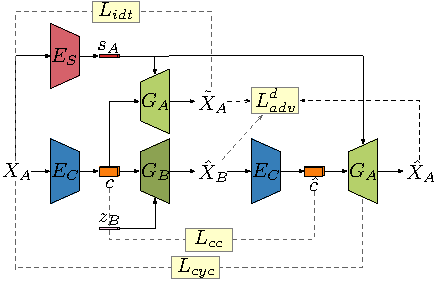
\includegraphics[width=1\textwidth]{figures/G.pdf}
    \caption{水下图像多模态转译模型MUGAN转译器网络结构。}
    \label{fig:mugan_g}
\end{figure*}

我们设置图像集$A$和$B$分别为空中域和多模态水下域。输入不配对的图像$x_A \in A$和$x_B \in B$,我们的目标是训练一个网络结构使得网络结果能够学会生成目标域$B$的多模态结果,且多模态结果对应于输入图像$A$的内容。多样的域风格向量可以来自目标域分布的随机采样也可以来自给定图像编码。

图~\ref{fig:mugan_g}和图~\ref{fig:mugan_d}所示为水下图像多模态转译模型MUGAN网络结构。MUGAN网络结构基于分解表达学习,图~\ref{fig:mugan_g}是转译模型结构,图~\ref{fig:mugan_d}是判别结构。转译模型包括编码器和生成器,生成器结构有两个分支,上分支整体来看是一个编码器-解码器结构,下分支整体是一个类似CycleGAN的循环网络,目的是训练模型实现跨域转译。

\begin{figure*}[ht]
    \centering
    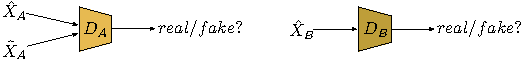
\includegraphics[width=1\textwidth]{figures/D.pdf}
    \caption{水下图像多模态转译模型MUGAN判别器网络结构。}
    \label{fig:mugan_d}
\end{figure*}

\textbf{编码器。}编码器包括两个,一个是内容编码器,一个是风格编码器。给一张来自空中域的图像$x_A$或者水下多模态域的图像$x_B$,风格编码器$E_S$提取给定图像的风格编码$s_A$或者$s_B$,其中$s_A = E_S(x_A)$,$s_B = E_S(x_B)$。内容编码器$E_C$将图像编码至内容空间$C$中。如图~\ref{fig:mugan_g}所示,内容编码器$E_C$将$x_A$编码成内容向量$c$,来自$\hat{x_B}$的向量$\hat{c}$理论上跟来自$x_A$的向量$c$是一致的,只是域风格信息不一致。$E_S$是一个MLP映射网络,$E_C$是一个包括三个卷集模块和四个残差模块的网络。

\textbf{生成器结构。}我们的生成器$G_A(\cdot)$和$G_B(\cdot)$将输入的内容和风格转译到目标域,目标域具有的特定风格特征信息可以来自目标域特定分布的采样$z_A$和$z_B$或者风格编码器提取的风格编码$E_S(\cdot)$。我们生成器包挎四个残差模块和两个上采样模块。我们对上采样模块和残差模块分别使用实例归一化(IN)和自适应实例归一化(AdaIN)~\cite{huang2017arbitrary}。风格信息通过全部AdaIN层注入,通过学习仿射变换进行缩放和移动向量。

\textbf{判别器结构。}判别器$D_A$和$D_B$都是PatchGAN~\cite{isola2017image}网络。判别器$D_A$用来判断输入图像$x$是来自$A$域的真实样本还是$A$域生成器$G_A$的生成结果$G_A(c,s_A)$,相应地判别器$D_B$是用来判断输入图像$x$是来自$B$域的真实样本还是$B$域生成器$G_B$的生成结果$G_B(\tilde{c},z_B)$。

\subsection{目标函数和算法}
$A$域和$B$域分别为空中域和水下多模态域,给定图像$x_A \in A$和输入目标域风格随机采样编码$z_B$,我们训练从$A \rightarrow B$的方向上的转译,其中用到的目标函数如下所示。

\textbf{域对抗损失.} 训练过程中,翻译器网络输入纯净完整的内容信息和目标域风格信息,通过域对抗损失限制翻译器学习生成目标域结果

\begin{equation}
\label{equ:adv_a_}
\mathcal{L}_{adv}^{\tilde{x}_A} = \mathbb{E}[\log D_A(x_A)] + \mathbb{E}[\log(1-D_A(G_A(c,s_A)))]
\end{equation}

\begin{equation}
\label{equ:adv_a}
\mathcal{L}_{adv}^{\hat{x}_A} = \mathbb{E}[\log D_A(x_A)] + \mathbb{E}[\log(1-D_A(G_A(\hat{c},s_A)))]
\end{equation}

\begin{equation}
\label{equ:adv_b}
\mathcal{L}_{adv}^{\hat{x}_B} = \mathbb{E}[\log D_B(x_B)] + \mathbb{E}[\log(1-D_B(G_B(c,z_B)))]
\end{equation}

生成器$G_A$学习使用来自$A$域的风格样式$s_A$生成$A$域具有足够真实性的图像$G_A(c,s_A)$和$G_A(\hat{c},s_A)$,企图可以混淆真实图像和生成结果,让$A$域判别器$D_A$无法区分他们。类似地,生成器$G_B$学习使用目标域分布采样编码$z_B$合成$B$域具有真实性的图像结果$G_B(c,z_B)$,目标也是让$B$域判别器$D_B$无法区分输入是真实图像还是生成假结果。

\textbf{循环一致性损失.}为了保证$A \rightarrow B$和$B \rightarrow A$两个方向上映射是循环一致的,我们使用CycleGAN~\cite{zhu2017unpaired}中提出的循环一致性损失来进行限制。

\begin{equation}
\label{equ:cycle}
\mathcal{L}_{cyc} = \mathbb{E}[\| G_A(\hat{c}, s_A) - x_A \|_1]
\end{equation}

其中$G_A(\hat{c}, s_A)$是$x_A$的重建结果。

\textbf{同一性损失。}我们在真实样本和生成结果$G_A(c,s_A)$之间采用同一性映射

\begin{equation}
\label{equ:idt}
\mathcal{L}_{idt} = \mathbb{E}[\| G_A(c, s_A) - x_A \|_1]
\end{equation}

当编码器成功地将输入图像分解成内容和风格两部分信息,理论上输入的真实数据应该跟合成的$G_A(c,s_A)$之间的距离非常接近。该损失保证生成器$G_A(\cdot)$生成$A$域的风格,不会自主地修改图像的色调,使得整体的风格产生变化。

\textbf{内容一致性损失。}为了保证从源域到目标域的跨域转译过程中内容保持完整,目标函数加入内容一致性损失,即真实样本和生成结果经过内容编码器分解得到的内容向量所包含的信息应该是一致的。

\begin{equation}
\label{equ:cc}
\begin{aligned}
\mathcal{L}_{cc} & = \mathbb{E}[\| E_C(G_A(c, s_A)) - E_C(x_A) \|_1] \\
       & = \mathbb{E}[\| \hat{c} - c \|_1]
\end{aligned}
\end{equation}

\textbf{KL损失。}KL损失致力于将分解后的内容和风格表达对齐高斯先验分布。

\textbf{总目标函数。}我们总的目标函数可以概括如下:

\begin{equation}
\label{equ:full}
\begin{aligned}
\min_{E,G}\max_{D} & \mathcal{L}_{adv}^{\tilde{x}_A}+\mathcal{L}_{adv}^{\hat{x}_A}+\mathcal{L}_{adv}^{\hat{x}_B} \\
+&\lambda_{cyc}\mathcal{L}_{cyc}+\lambda_{idt}\mathcal{L}_{idt}+\lambda_{cc}\mathcal{L}_{cc}+\lambda_{kl}\mathcal{L}_{kl}
\end{aligned}
\end{equation}

其中$\lambda_{cyc}$,$\lambda_{idt}$,$\lambda_{cc}$和$\lambda_{kl}$是对应每单项损失的超参数。后续除了分布采样向量,我们还用引导图像经过经过风格编码器后得到风格编码来测试我们模型的有效性。我们默认设置这些参数分别为$10$,$5$,$1$,$0.01$。

\section{水下图像多样式域转译设计}
在这一节,将对该问题进行分析,提出模型设计思路,设置目标函数,为下一章节中的实验提供理论依据和实验意义。

\subsection{问题及分析}
我们将给定图像转译到水下环境的多样式域的图像转译称为水下图像多样式域转译。基于生成对抗网络,我们想通过一个网络结构,在无监督的条件下,实现水下图像多样式域的图像转译。受UIE-DAL方法启发,通过对多个水下条件进行编码,从而对多个样式域进行控制,实现到多个样式域的转译。

对图像转译中的经典方法综述。CycleGAN是经典跨域转译方法,通过循环一致性损失成功实现两个域之间的双向转译,想要实现多域之间的转译,只能一一之间进行训练,若有$n$个域之间转译,需要训练$n(n-1)/2$次。StarGAN解决了多域转译的问题,只使用一个生成器来实现多个域之间的生成。在StarGAN中,并不使用传统的固定转译,而是将域信息和图片一起输入进行训练,并在域标签中加入编码向量,便于不同的训练集进行联合训练。通过加入每个域设置的标签,对应的把生成图片变到指定的域。StarGAN v2在StarGAN实现多域转译的基础上,同时解决生成图像的多样性和在多个域上的可扩展性的问题。以StarGAN为基础,用特定域的样式代码替换原来的域标签,这些代码可以表示特定域的各种形式。StarGAN v2引入两个模块,一个映射网络将随机高斯噪声转换为样式代码和一个样式编码器从给定的参考图像中提取样式代码。DRIT++在DRIT两个域多模态转译的基础上拓展至多个域之间的图像转译。给每个域进行one-hot编码,加入域分类损失,以区分不同域。在作者给出的代码中单独为多域转译任务建立一个项目称MDMM,后续会用MDMM作为DRIT++工作中多域转译方法。

%这些方法测试结果中存在的问题。
%我们设置的方法好处
在用多域转译方法解决我们转译到水下多个样式条件下图像问题时,我们设计了一个多域转译模型。使得在转移过程中目标内容保持不变,多个样式域仅仅改变图像中的水下环境条件。在不需要配对数据的情况下,给定要转译的多个域图像,通过对各个域进行编码作为域控制条件,实现到多个样式域的转译任务,对数据配对没有要求,有很强的泛化能力。

\subsection{模型结构}

\begin{figure*}[ht]
    \centering
    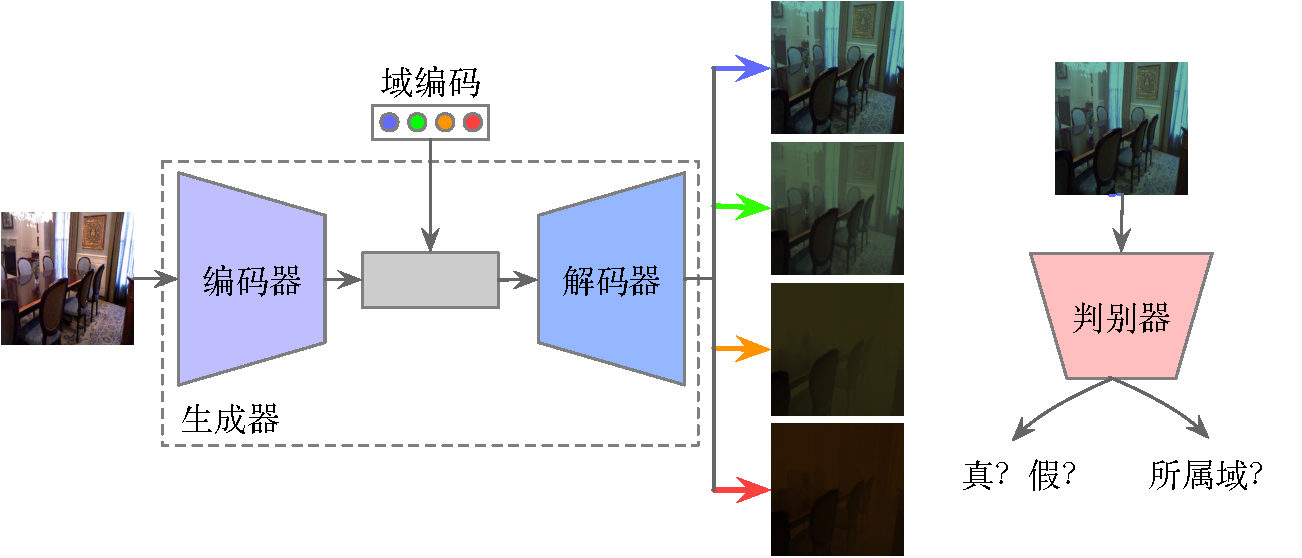
\includegraphics[width=1\textwidth]{figures/Domain_network.pdf}
    \caption{水下图像多样式域转译网络结构。}
    \label{fig:domain_net}
\end{figure*}

我们设置输入数据Input,其他样式的数据分别作为$A$,$B$、$C$、$D$等依次顺序排列域。我们的目标是通过网络结构使得输入能够学会转译到各个域中,其中转译结果中的内容跟输入保持一致,不同的域之间只有样式发生变化,样式可以是浑浊度、颜色等视觉效果变量。

\subsection{目标函数和算法}
我们





\section{实验环境}
整个网络使用Pytorch框架,计算机环境CPU型号为Intel$^\circledR$ Core$^{\text{TM}}$ i5-8500 CPU,操作系统为Ubuntu 16.04 LTS版本,显卡型号为Nvidia GeForce GTX 1070,内存128GB,显存为8GB。

本工作中使用的基准方法模型使用官方Github中给出的Pytorch版本代码进行实验。根据代码中需要的依赖包,使用Anaconda创建和控制相应的虚拟环境实验。为了彰显公平,在选取基准方法时,全部选择给出完整版本代码的方法进行对比。

\section{本章小结}

\chapter{水下图像合成实验与分析评测}
本章将针对水下图像多模态转译问题设计实验、确定评价指标,验证我们设计的网络模块的有效性,并与基准方法进行对比和分析。

\section{水下图像跨域多模态合成实验设计}
\subsection{实验设置}
基准方法我们总共选取了五种,其中两种经典的图像转译方法CycleGAN~\citep{zhu2017unpaired}和基于分解表示的跨域多模态转译方法MUNIT~\citep{huang2018multimodal},三种最新的图像多模态转译方法DRIT++~\citep{lee2020drit++}、DSMAP~\citep{chang2020domain}和StarGAN v2~\cite{choi2020stargan}。除了不可或缺的经典模型CycleGAN,剩余四种方法都可以完成两个域之间的多模态转译任务。

CycleGAN学习两个域之间的一对一映射,通过循环一致性损失能够很好的学习到目标域的特征;MUNIT, DRIT++ and DSMAP将图像分解为共享的内容空间和不同域的特征空间,然后通过给生成器共享的内容和目标域的特征合成目标域风格相同内容信息的结果;StarGAN v2使用一个生成器结构,通过编码控制生成具有多个特征的多个目标域。所有基准方法的训练代码均来自作者Github提供完成版本。

在我们的实验室中,将$A$域设置为空中域,$B$域设置为多模态水下域,在以上五种基准方法上进行多个数据集的客观实验。在真实水下数据集和合成数据集上设置了针对模糊程度、水颜色、以及特定水质状态的多个实验。

\subsection{数据集设置}
由于水下环境导致采集数据限制,我们的数据集并不是十分充足,因此在一种实验实验设置中用到多个数据集的组合结果。我们在水下图像多模态转译任务中,主要使用到RUIE~\citep{liu2019real}, UWCNN~\citep{li2020underwater}, UVB 2017数据集。EUVP~\citep{islam2019fast}和UIEB~\citep{li2019underwater}数据集就作为补充进行组合实验。其中RUIE,UIEB和EUVP部分数据集是真实世界水下图像结果,UWCNN和UVB 2017是合成图像结果。这些数据集在各个子集数量上并不都是均衡的,所以训练时对模型方法提出了较高的要求。

\begin{figure*}[htp]
    \centering
	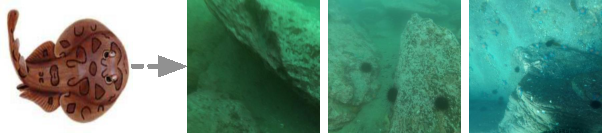
\includegraphics[width=\textwidth]{figures/ruie-dataset.pdf}
	\caption{RUIE数据集多模态转译示例。}
	\label{fig:ruie_dataset}
\end{figure*}

RUIE数据集是一个真实世界获取到的水下不配对图像集。如图~\ref{fig:ruie_dataset}所示,当我们进行水下色偏和清晰度实验训练时,选择RUIE的子集UCCS的300张图片当作水下域,选取EUVP中300张无水子集作为空中域。进行测试实验时,选择EUVP中的100张无水图像作为空中域,测试训练模型,以获得水下多模态域的结果。

\begin{figure*}[htp]
    \centering
	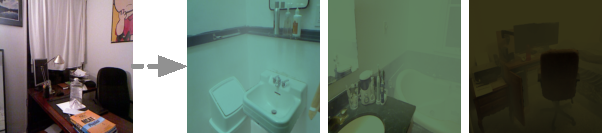
\includegraphics[width=\textwidth]{figures/uwcnn-dataset.pdf}
	\caption{UWCNN数据集多模态转译示例。}
	\label{fig:uwcnn_dataset}
\end{figure*}

UWCNN数据集使用NYU-v2的RGB-D图像来合成深海和近海的十种水类型。基于水下衰减模型,多个衰减系数当作不同的水类型的控制变量。如图~\ref{fig:uwcnn_dataset}所示,当我们进行训练时,选择1200张衰减系数为0即无水域,选择近海type-1,type-3,type-5,type-7作为水下多模态域,每种类型选取300张,这几种水下类型在视觉上有直观可见的区别,方便后续进行定性评价。进行测试时,选择无水域中249张进行测试。

\begin{figure*}[htp]
    \centering
	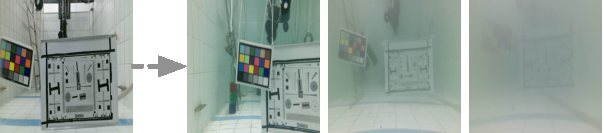
\includegraphics[width=\textwidth]{figures/uvb-dataset.pdf}
	\caption{UVB数据集多模态转译示例。}
	\label{fig:uvb_dataset}
\end{figure*}

Underwater Vision Benchmark 2017 (UVB 2017)是我们实验室用ZED和Kinect立体摄像机捕获的图像和视频数据集。在大连进行了模拟浑浊度实验,将不同浓度的\ce{Al(OH)3}模拟不同水质类型的浑浊度,相机收集相同目标物在不同距离和不同水质下的多种结果。如图~\ref{fig:uvb_dataset}所示训练时,我们选择了66张作为无水域,447张不同深度和浑浊度的结果作为水下多模态域。测试时,无水域选取66张进行测试。

\subsection{评价准则}
为了方便对各个方法进行客观对比,在图像转译角度从转译结果真实性、多样性来进行评价。

\textbf{真实性。}真实性是指给定源域$x_A$图像作为输入,生成的结果应该域目标域$x_B$中的分布尽可能的相同。在我们实验中,生成的水下多模态域的结果应该在质量真实性评价上尽可能的相近。

我们在实验中,真实性指标选取Fréchet Inception Distance(FID)来进行评价。基于Inception score改进,FID最初由Heusel等人~\cite{heusel2017gans}提出。与Inception分数一样,FID分数也使用了Inception v3模型。具体而言,模型的编码层(图像的分类输出之前的最后池化层)被用来抽取输入图像的用计算机视觉技术指定的特征。这些激活函数是针对一组真实图像和生成图像计算的。
使用来自 Inception v3 模型的激活函数输出来归纳每个图像,得分即为Frechet Inception Distance。FID能够完善Inception score没有比较模型生成样本和真实样本统计特性的问题。FID 越低,图像质量越好;反之,得分越高,质量越差,两者关系应该是线性的。较低的FID意味着两个分布之间更接近,也就意味着生成图片的跟真实结果之间相似性较高。

\textbf{多样性。}非成对图像多模态转译问题中,在输入唯一时,能产生目标域的多模态结果。在我们到水下图像多模态转译任务中,在输入一张空中图像时,我们希望能得到多个对应的水下域图像转译结果。即使都是相同的内容,在水质等水下条件不同导致水下图像的模态不一致。对于生成的多种图像,都能跟输入图像拥有相同的内容,再对生成结果进行多样性的评价。

\begin{figure*}[htp]
    \centering
	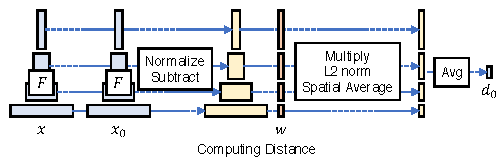
\includegraphics[width=\textwidth]{figures/LPIPS.pdf}
	\caption{}
	\label{fig:lpips}
\end{figure*}

在实验中,我们选用Learned Perceptual Image Patch Similarity (LPIPS)来评价多样性指标。LPIPS最初由Zhang等人~\cite{zhang2018perceptual}提出,相比于传统的图像相似度评价指标,LPIPS指标得到的结果和人的视觉评价有更高的相关性。LPIPS用来评价生成结果的多样性,用预训练好的AlexNetAlex~\cite{krizhevsky2017imagenet}网络来提取特征后计算$L_1$距离。对于每个测试图像,用指定个随机采样的潜在向量来生成指定个数的输出结果,对于同一个输入的多个结果对之间计算平均距离,最后所有测试输入的均值,并把这个数值当作LPIPS结果。

\section{水下图像跨域多模态合成结果分析}
\subsection{定性结果分析}

\begin{figure*}[htp]
    \centering
	\includegraphics[width=\textwidth]{figures/RUIE_random_1.pdf}
	\caption{在RUIE数据集上,基准方法和我们提出的方法在目标域随机采样生成的多模态结果比较。}
	\label{fig:ruie_random_1}
\end{figure*}

\begin{figure*}[htp]
    \centering
	\includegraphics[width=\textwidth]{figures/RUIE_random_2.pdf}
	\caption{在RUIE数据集上,基准方法和我们提出的方法在目标域随机采样生成的多模态结果比较。}
	\label{fig:ruie_random_2}
\end{figure*}

图~\ref{fig:ruie_random_1}和图~\ref{fig:ruie_random_2}展示了不同方法在RUIE数据集上的定性结果对比。第一行Real图像表示模型输入图像,之后每行都是对应标记方法获得的结果。从对比图中可以看到,CycleGAN+noise方法的转译结果比较真实,内容信息保留完整,但是噪声被忽略,不同风格采样信息加入的每行之间没有多模态样式的结果;MUNIT方法转译结果质量较差,内容丢失了大量的信息,内容轮廓信息几乎全部丢失,尽管模态之间能看出区别,从行结果上看同样的风格采样信息影响的风格样式并没有一致;DSMAP方法中每行风格信息影响的样式上能看出一致的差异,很明显内容和风格也没有分解彻底,DSMAP的内容收风格样式的影响很严重,在内容细节上没有多少保留,可以看出DSMAP对于内容的处理非常粗糙,生成结果边缘也有伪影的出现。DRIT++方法的结果,内容轮廓能够得到有效的保留,具体内容细节丢失十分严重,DRIT++有多模态效果,但每行模态没有没有实现一致的效果;StarGAN v2方法生成的结果很差,视觉上是学习到了海底样式,但是内容没有有效保留并控制模态样式变化,通过训练没有成功学习到并实现我们想要的多模态转译任务。而本文提出的多模态转译方法,简洁有效的将内容信息和风格信息进行拆分,在内容上,能够极好的保留目标物和水纹理等轮廓和目标颜色变化等细节,在风格上,每行相同风格信息输入能够实现每行风格样式结果的一致,定性视觉上,真实有效地实现水下图像多模态的合成。

\begin{figure*}[htp]
    \centering
	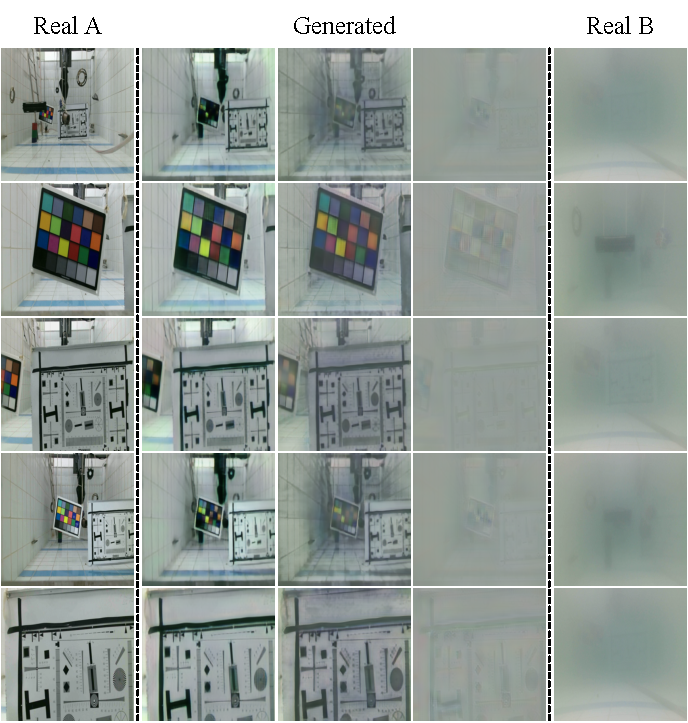
\includegraphics[width=\textwidth]{figures/UVB_random.pdf}
	\caption{在UVB 2017数据集上,基准方法和我们提出的方法在目标域随机采样生成的多模态结果比较。}
	\label{fig:uvb_random}
\end{figure*}

图~\ref{fig:uvb_random}展示了不同方法在UVB 2017数据集上的定性结果对比。第一行Real图像表示模型输入图像,之后每行都是对应标记方法获得的结果。从对比图中可以看到,CycleGAN+noise方法的转译结果较为真实,在浑浊度变化的UVB 2017数据集上尽管内容保持较为完整,像色卡这种比较直观的目标物可以看出转译结果在色卡颜色上保留较好,但是色卡轮廓发生了扭曲,而且没有模态上的变化,噪声对于模态的影响在肉眼上无法辨别;MUNIT方法转译结果内容上可以较好的保留,在目标物轮廓上依旧会发生形变,导致目标物视觉上扭曲,在风格样式上,对于较近的目标物,模糊程度的变化不明显,对于较远的目标物,能够明显看出浑浊程度在不同模态样式上发生了变化,会出现数据集中模糊不存在的绿色雾状效果,越远的位置绿色雾状效果越明显;DSMAP方法转译结果类似MUNIT转译结果,在目标物在内容上会发生形变,在色卡各个颜色之间的扭曲会比MUNIT更明显,整体在内容上不够完整但保留度可以接受,在风格上,一样会出现不存在的绿色雾状效果,呈现近处白色模糊远处绿色模糊的效果;DRIT++方法转译结果,内容上不能保留让人满意的结果,对于内容轮廓能够很好的进行保留,但是对于内容信息,没有得到有效的重视,对于颜色比较复杂的内容部分,直接被黑色阴影填充,导致内容没有完整保留,风格基本上都是水下域中的白色模糊,却会出现棋盘网格样式,是网络结构设计导致的问题;StarGAN v2方法转译结果,在UVB 2017数据集上能有比RUIE真实水下数据集明显成功的转译结果,可以看出StarGAN v2对于数据集本身有一定的要求,在UVB 2017数据集上,内容可以基本保留完整,在色卡上可以看出有轻微的扭曲变形,但是颜色基本保持完整,对于远处的目标物形状基本也完整,风格样式上,视觉效果不明显,多行之间无法清楚辨认出是来自不同模态的结果。而本文提出的水下图像多模态转译方法,内容能够几乎全部被完整保留,不论位置较近还是较远的目标物颜色都没有发生改变仅有模态导致的一定程度模糊、形状也是无扭曲的保留,三个模态的三行结果可以明显看出有样式上的区别,且每个模态影响的风格样式都保持了不同目标上的一致性。可以明显的看出我们的模型在UVB 2017数据集上也可以展现较好的效果。

\begin{figure*}[htp]
    \centering
	\includegraphics[width=\textwidth]{figures/UWCNN_random.pdf}
	\caption{在UWCNN数据集上,基准方法和我们提出的方法在目标域随机采样生成的多模态结果比较。}
	\label{fig:uwcnn_random}
\end{figure*}

图~\ref{fig:uwcnn_random}展示了不同方法在UWCNN数据集上的定性结果对比。第一行Real图像表示模型输入图像,之后每行都是对应标记方法获得的结果。CycleGAN+noise方法的转译结果真实度较高,对于输入图像中的内容保存完好,可以看出生成结果不存在多模态样式,且噪声被模型忽略,无法扰动生成网络从而合成多模态结果;MUNIT在UWCNN数据集上生成的结果较为真实,内容也保存比较完好,但是在生成结果中,色彩较多的部分(如图~\ref{fig:uwcnn_random}MUNIT生成结果中茶几上的部分)会出现转译失败的情况,生成结果能出现多模态效果,每行同一种风格样式编码无法控制模态一致性;在MUNIT方法上进行改进的DSMAP方法转译效果有明显的提升,在内容上基本保留完整,仔细看细节会有轻微的变形,图像中的物体轮廓形状发生了扭曲,对于每行同样的风格编码输入,能有整齐一致的模态变化,在风格上的转译是十分成功地,唯一的缺憾就在于内容没有保持原有的形态;DRIT++方法转译结果,部分内容损失严重,其中轮廓变得模糊,没有清晰的边界,对于雾较为浓厚的模态这种问题不明显,对于雾轻薄的地方,内容的损失就很清晰的展现出来,风格上能有多模态样式,对于每行同一风格编码输入,不能合成一致的模态样式;StarGAN v2结果基本内容能够保存完整,除了内容轮廓有轻微扭曲,整体内容较为完整,且雾与数据集中展示的距离越远的地方雾越厚一致,风格上能生成多模态效果,每行模态效果相似,但不能完全一致,整体风格能看出多模态效果。本文提出的方法在内容上保存完整,无论是内容细节还是内容轮廓都没有发生变化,颜色信息也能在合成过程中保留,对于每行不同的风格编码,每行能有一致的风格样式,且模态间有明显区别的多模态结果。本文提出的方法不仅对于真实水下图像,对于合成水下图像一样能进行有效的多模态控制。


\begin{figure*}[ht]
    \centering
	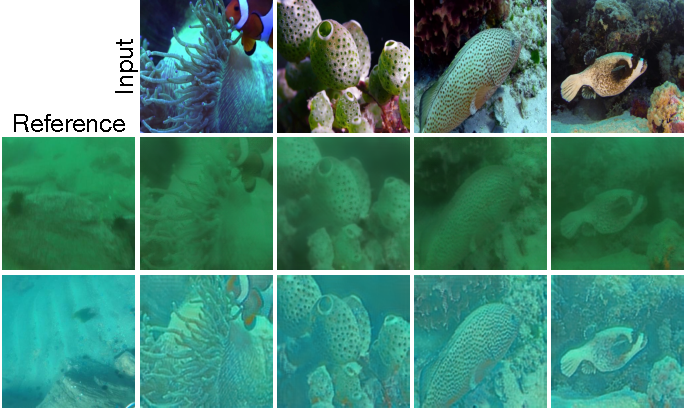
\includegraphics[width=\textwidth]{figures/RUIE_guidance.pdf}
	\caption{RUIE数据集上,本文提出方法用参考图像引导生成指定模态的结果。}
	\label{fig:ruie_guide}
\end{figure*}

图~\ref{fig:ruie_guide}展示了本文提出方法在参考图像引导方式上的多模态结果。对于输入图像,我们给出明确的参考风格图像,将参考图像编码成可以被生成器获取到的风格编码,如此可以合成指定参考风格的合成结果。从每一列可以看出,输入图像的内容得到了很好的保留,细节和轮廓都没有发生任何损失,从每行可以看出,风格影响的水质和模糊程度在不同输入图像上也影响一致。这说明,本文提出的方法能够有效的将图像中的内容和风格进行拆解,内容信息作为恒定不变的部分,在转移过程中需要完整的保留,风格信息作为模态的控制变量,在转译时,源风格信息要彻底清除,且被目标风格替换带入转译过程。

\begin{figure*}[ht]
    \centering
	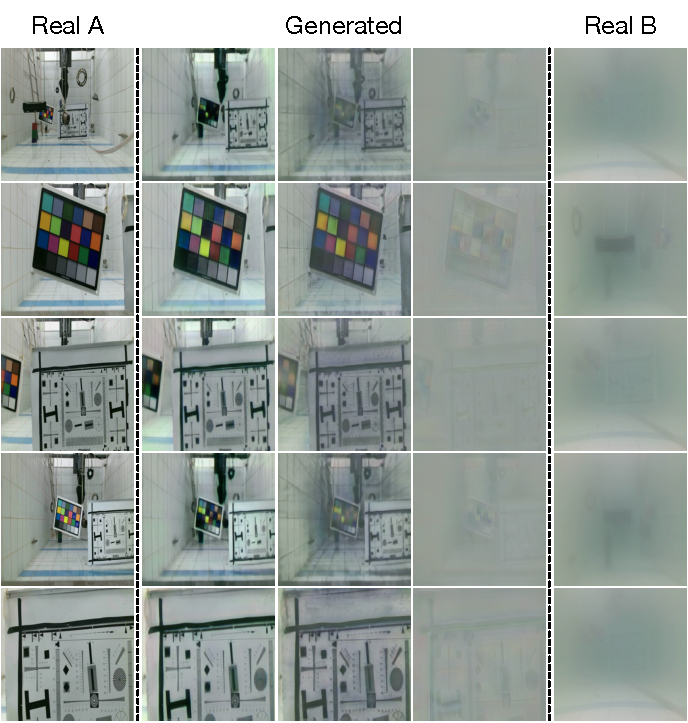
\includegraphics[width=\textwidth]{figures/UVB-change.pdf}
	\caption{在UVB 2017数据集上,浑浊程度样式逐步变化过程。}
	\label{fig:uvb-change}
\end{figure*}

图~\ref{fig:uvb-change}展示了本文提出方法在UVB 2017数据集模态逐步变化过程中的效果。图中Real A代表输入图像,Real B代表目标图像,中间为模态生成结果。我们的方法除了如图~\ref{fig:ruie_guide}中展示的让输入图像A生成目标图像B模态下的结果外,还可以合成逐步从模态A样式变化至模态B样式的结果。A是水下没有浑浊的图像,B是水下浑浊明显的图像,从生成的结果中可以看到,生成图像从左往右依次变化过程中,浑浊度不断增加,趋向于B中浑浊程度。在生成结果中,模态逐步变化,图像中的内容保持不变,仅仅是浑浊程度这个样式上发生了改变,内容的颜色、细节和轮廓都保存完整。

\subsection{定量结果分析}

真实性和多样性定量指标如表~\ref{tab:ruie_comparison}、~\ref{tab:uvb_comparison}和~\ref{tab:uwcnn_comparison}所示。在定量结果分析,我们对比了CycleGAN、MUNIT、DRIT++、DSMAP、StarGAN v2基准方法在RUIE、UVB 2017和UWCNN数据集上的实验评价,所有方法都是用作者Github代码给出的标准测试,采用相同指标的标准评价,下列结果能够客观的进行对比分析。

\begin{table*}[ht]
\centering
\caption{在RUIE数据集上,基准方法和我们方法的真实性和多样性定量比较。}
  \begin{tabular}{c|ccccccccc}
    \hline\noalign{\smallskip}
    方法 & CycleGAN+noise & MUNIT & DRIT++ & DSMAP & StarGAN v2 & Ours \\
    \noalign{\smallskip}\hline\noalign{\smallskip}
    FID$\downarrow$ & 143.4 & 139.4 & 179.2 & 139.6 & 121.1 & \textbf{83.2} \\
    LPIPS$\uparrow$ & 0.534 & 0.452 & 0.575 & 0.513 & 0.431 & \textbf{0.579} \\
    \noalign{\smallskip}\hline
  \end{tabular}
  \label{tab:ruie_comparison}
\end{table*}

从表格~\ref{tab:ruie_comparison}中我们可以看到,在真实水下获取到的RUIE数据集上从空中到水下多模态域转译的定量结果对比。CycleGAN+noise方法评价中,FID指标较高,说明跟真实水下图像差距较大,分析原因主要是因为CycleGAN+noise生成结果较为固定,跟真实多模态样本之间会存在较大的差异,输入图像的合成结果加上噪声也没有多模态样式,但是自身转译结果是真实样本多模态样式中的任意一种,在计算LPIPS指标时,结果看起来令人满意,实际上同一输入无法产生多模态结果;MUNIT方法评价中,FID指标较高,说明跟真实水下图像差距较大,这主要是由于合成结果中内容损失严重,内容在轮廓上都无法与模态样式分离,在计算LPIPS指标时,能生成多模态效果但是模态之间效果差别较小,多样性不够多导致LPIPS指标较低;DRIT++方法评价中,由于合成的结果内容细节信息丢失严重,在与真实样本计算FID指标时,必然会有很巨大的差距,所以FID指标最高,真实性最差,在计算LPIPS指标时,对于不同的风格采样,同一输入可以生成不同模态养的结果,因此多样性足够高,可以看出与我们方法指标相差无几,但是对于每种特定的风格采样,不同输入无法生成一致模态的结果;DSMAP方法是在MUNIT方法上进行改进,将域共享内容信息拆分出域特有内容信息,实际上将内容和风格进一步分解,这样获得到的内容信息更加纯净,在测量指标时,由于合成结果内容损失严重,除了部分轮廓能辨认其余内容信息全部丢失,在计算FID时,跟真实样本结果之间的差异必然巨大,导致FID指标较高,在计算LPIPS指标时,输入每种模态风格能有一致的合成模态结果,因此多样性存在;StarGAN v2方法评价中,由于生成结果内容没有有效保留,但是学习到了海底样式,所以在评价FID指标时,结果稍微有点高,存在多模态效果但是模态之间差异不明显,在评价LPIPS指标时结果较低,多样式不足。本文中提出的方法评价中,生成结果内容保留完好,且合成结果接近真实样本,所以FID结果较低,说明合成结果真实性高;能够通过对目标域风格随机采样或者通过参考图像进行引导合成真实的多模态结果,有足够多的模态样式,所以LPIPS指标最高,说明合成结果多样性充足。

\begin{table*}[ht]
\centering
\caption{在UWCNN数据集上,基准方法和我们方法的真实性和多样性定量比较。}
  \begin{tabular}{c|ccccccccc}
    \hline\noalign{\smallskip}
    方法 & CycleGAN+noise & MUNIT & DRIT++ & DSMAP & StarGAN v2 & Ours \\
    \noalign{\smallskip}\hline\noalign{\smallskip}
    FID$\downarrow$ & \textbf{80.7} & 232.1 & 290.7 & 138.8 & 149.8 & 129.6          \\
    LPIPS$\uparrow$ & 0.490         & 0.647 & 0.668 & 0.513 & 0.595 & \textbf{0.736} \\
    \noalign{\smallskip}\hline
  \end{tabular}
  \label{tab:uwcnn_comparison}
\end{table*}

从表格~\ref{tab:uvb_comparison}中我们可以看到,在合成数据集UWCNN空中到水下多模态图像域转译的定量结果对比。CycleGAN+noise方法测评中,图像真实性非常高,跟数据集中部分模态真实样本分布接近,在计算FID时,CycleGAN+noise和真实数据之间的差距非常小,在计算LPIPS时,由于该方法合成的样本不受风格编码的扰动,合成样本的多样性缺乏,因此LPIPS指标较低;MUNIT方法测评中,图像内容上可以较好的保 留,在目标物轮廓上依旧会发生形变,导致目标物视觉上扭曲,在计算FID时,差异较大,扭曲导致真实性下降,在计算LPIPS时,能看出模态在不同风格编码输入时发生变化,所以LPIPS指标较高,多样性结果存在;DSMAP方法测评中,类似MUNIT会发生形变,且扭曲比MUNIT更严重,所以在计算FID时结果值较高,真实性更低,在计算LPISP时,不同输入之间的多模态样式不明显,导致多样性不足,指标较低;DRIT++方法测评中,由于内容信息中复杂的部分被黑色阴影填充,真实性降低,因此FID指标最高,由于不同的模态样式编码输入可以影响合成不同样式,有多样性结果,因此LPIPS值较高;StarGAN v2在UWCNN数据集上可以合成视觉上真实的结果,与真实样本分布较为接近,因此FID较低,但是在风格上缺乏多模态合成结果,因此LPIPS也比较低。本文提出的方法在合成结果中,内容信息保留完整,在所有基于分解的转译方法中,可以FID最低,且多种样式合成结果都有,多样性足够所以LPIPS可以获得最高值。

\begin{table*}[ht]
\centering
\caption{在UVB数据集上,基准方法和我们方法的真实性和多样性定量比较。}
  \begin{tabular}{c|ccccccccc}
    \hline\noalign{\smallskip}
    方法 & CycleGAN+noise & MUNIT & DRIT++ & DSMAP & StarGAN v2 & Ours \\
    \noalign{\smallskip}\hline\noalign{\smallskip}
    FID$\downarrow$ & \textbf{145.1} & 240.4 & 243.7 & 232.6 & 162.9 & 172.7          \\
    LPIPS$\uparrow$ & 0.358          & 0.486 & 0.474 & 0.444 & 0.358 & \textbf{0.493} \\
    \noalign{\smallskip}\hline
  \end{tabular}
  \label{tab:uvb_comparison}
\end{table*}

从表格~\ref{tab:uwcnn_comparison}中我们可以看到,在合成数据集UWCNN空中到水下多模态图像域转译的定量结果对比。CycleGAN+noise方法测评中,转译结果真实度较高,对于输入图像中的内容保存完好,在计算FID时,能够得到最低值,但是由于CycleGAN+noise生成结果不具有多样性,在计算LPIPS时结果较差;MUNIT生成的结果较为真实,内容也保存比较完好,会出现真实样本中不存在的黄色模态,且颜色较多的部分转译会失败,在计算FID时,与真实结果差别较大,真实性不高,FID值很高,在计算呢LPIPS时会出现多种模态样式,且模态间差别很大,所以LPIPS指标较高;DSMAP在内容上基本保留完,也出现了真实样本中不存在的黄色模态结果,FID指标较高,缺乏真实性,合成结果能在模态上出现多样性且模态内的一致性,LPIPS指标结果较高;DRIT++方法测评中,轮廓模糊,边界不清晰,与真实样本结果区别较大,FID指标最高,真实性最低,尽管模态内结果不一致,担合成结果有明显的模态差异,LPIPS指标较高,具有多样性;StarGAN v2结果基本内容能够保存完整,且合成模态非常近似真实样本,FID指标较低,真实性较高,风格上生成的多模态效果模态内不稳定,LPIPS指标较低,多样性不充足。本文提出方法测评中,内容上保存完整,在其他分解表达方法中可以得到最好的FID结果,真实性较高;真实样本中存在的多种样式合成结果都有,多样性充足所以LPIPS最高。

\subsection{消融实验}

为了验证我们设计网络的有效性,主要对于转译器部分进行模块验证。通过使用MUNIT和DRIT++的转译器来验证我们转译器结构的有效性;通过对比有无内容一致性损失限制的结果,验证我们提出内容一致性限制的有效性。

\begin{table*}[htbp]
  \centering
  \caption{在RUIE、UVB 2017和UWCNN数据集上,转译器结构的比价结果。}
    \begin{tabular}{c|c|c|c|c|c|c}
    \hline
    \multirow{2}[3]{*}{} & \multicolumn{2}{c|}{MUNIT} & \multicolumn{2}{c|}{DRIT++} & \multicolumn{2}{c}{Ours} \\
\cmidrule{2-7}          & \multicolumn{1}{c|}{FID$\downarrow$ } & \multicolumn{1}{c|}{LPIPS$\uparrow$} & \multicolumn{1}{c|}{FID$\downarrow$ } & \multicolumn{1}{c|}{LPIPS$\uparrow$} & \multicolumn{1}{c|}{FID$\downarrow$ } & LPIPS$\uparrow$ \\
    \midrule
    RUIE  & 88.0388 & 0.438 & 92.2588 & 0.462 & \textbf{83.2399} & \textbf{0.579} \\
    UVB  & 197.7265 & 0.469 & 181.7613 & 0.489 & \textbf{172.7404} & \textbf{0.493} \\
    UWCNN & 185.4869 & 0.627 & 185.1982 & 0.598 & \textbf{129.6982} & \textbf{0.736} \\
    \hline
    \end{tabular}%
  \label{tab:comp_G}%
\end{table*}%

表格~\ref{tab:comp_G}所示为对于转译器有效性的验证结果。在相同的网络框架下,对比了基于分解表达方法MUNIT、DRIT++转译器,用真实性和多样性指标FID和LPIPS共同验证我们转译器结构的有效性。从表格中可以看出,我们转译器合成的水下图像多模态结果在真实性和多样性上都优于同样基于分解表达学习的经典方法MUNIT和DRIT++。FID是所有转译器生成结果中最低的,最接近真实样本分布,LPIPS是所有转译结果中最高的,多样性丰富。

\begin{figure*}[htp]
    \centering
  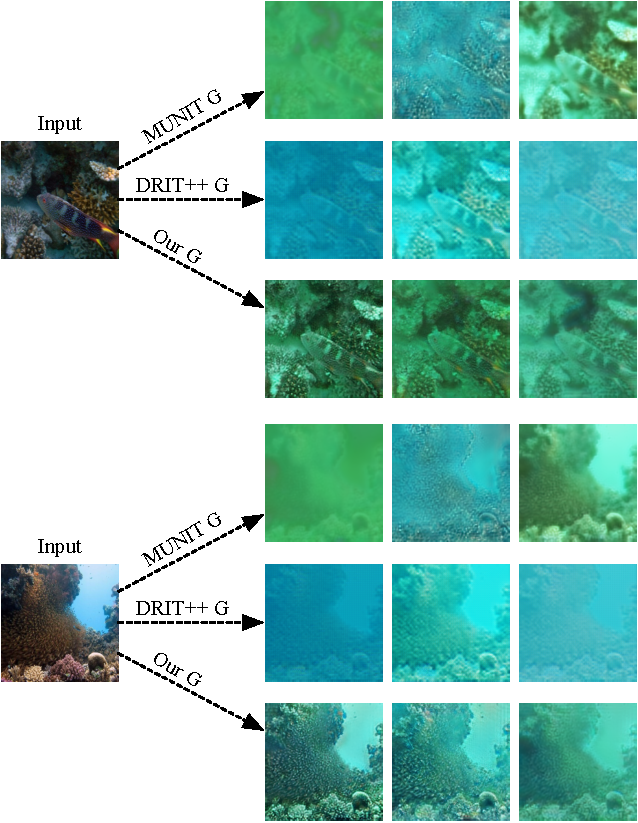
\includegraphics[width=\textwidth]{figures/Ablation_modal_ruie.pdf}
  \caption{RUIE数据集上,转译器有效性对比结果。}
  \label{fig:ablation_modal_ruie}
\end{figure*}

图~\ref{fig:ablation_modal_ruie}所示是RUIE数据集上本工作的转译器跟MUNIT、DRIT++转译器生成结果对比。在RUIE数据集上,我们对比了使用MUNIT、DRIT++转译器的生成结果。在多模态样式模糊程度和视觉效果任务下,MUNIT、DRIT++转译器在相同网络架构下,通过对目标域分布随机采样,生成多模态结果。其中各个方法都能成功生成多模态样式,在MUNIT和DRIT++中噪声对颜色样式造成影响十分明显。MUNIT方法中,内容损失很严重,在模态变化中,内容保存不完整,DRIT++中,内容能保留较为完整,但是三个模态中,颜色变化明显,针对模糊程度没有明显的变化。

\begin{table*}[htbp]
  \centering
  \caption{在RUIE、UVB 2017和UWCNN数据集上,转译器结构有无内容一致性限制结果。}
    \begin{tabular}{c|c|c|c|c|c|c}
    \hline
    \multirow{2}[3]{*}{} & \multicolumn{2}{c|}{RUIE} & \multicolumn{2}{c|}{UVB 2017} & \multicolumn{2}{c}{UWCNN} \\
\cmidrule{2-7}          & \multicolumn{1}{c|}{FID$\downarrow$ } & \multicolumn{1}{c|}{LPIPS$\uparrow$} & \multicolumn{1}{c|}{FID$\downarrow$ } & \multicolumn{1}{c|}{LPIPS$\uparrow$} & \multicolumn{1}{c|}{FID$\downarrow$ } & LPIPS$\uparrow$ \\
    \midrule
    Ours  & 83.2399 & 0.579 & 172.7404 & 0.493 & 129.6982 & 0.736 \\
    Ours w/o $\mathcal{L}_{cc}$ & 85.0344 & 0.575 & 175.3312 & 0.499 & 129.8680 & 0.724 \\
    \hline
    \end{tabular}%
  \label{tab:ablation_modal_lcc}%
\end{table*}%

表格~\ref{tab:ablation_modal_lcc}所示为转译器有无内容一致性损失$\mathcal{L}_{cc}$的对比结果,在RUIE、UVB 2017和UWCNN数据集上都进行了对比实验。在对比结果中我们可以看到,在有内容一致性损失$\mathcal{L}_{cc}$时,我们的结果在真实性和多样性上都有比较稳定的结果,当没有内容一致性损失$\mathcal{L}_{cc}$时,生成结果中的内容保留不如有内容一致性损失$\mathcal{L}_{cc}$的结果,所以在FID较高,真实性不如有内容一致性损失$\mathcal{L}_{cc}$结果的真实性,但是在多样性上,内容一致性损失$\mathcal{L}_{cc}$对最终的结果影响不大,所以LPIPS结果接近。

\section{水下图像多样式域合成实验设计}
\subsection{实验设置}
基准方法我们总共选择了三种,经典无监督跨域图像转译方法CycleGAN~\cite{zhu2017unpaired},两种最新颖的多域转译模型StarGAN v2~\cite{choi2020stargan}和MDMM~\cite{lee2020drit++}(DRIT++中拓展至多域转译任务Github项目)。其中,跨域转译模型CycleGAN可以学到两个域一对一的映射,在进行多域转译时,需要域两两之间进行训练,无法一次同时实现多个域的训练。

CycleGAN可以看成两个GAN的融合,两个网络构成循环过程通过循环一致性损失,实现无监督的跨域转译;MDMM依旧使用分解的方式,用一个生成器实现多个域的转译,给定其中两个域的图像和one-hot编码,分解到共享内容空间和域特有风格空间,类似DRIT跨域转译方式进行训练;StarGAN v2是在多域转译模型StarGAN

\subsection{数据集设置}
由于水下图像数据限制,在多域转译任务中我们实验同样会用到多个数据集组合。在水下多样式域转译任务中,主要使用RUIE~\cite{liu2019real},UWCNN~\cite{li2020underwater},UVB 2017数据集,另外使用EUVP~\cite{islam2019fast},UIEB~\cite{li2019underwater}作为补充数据集,在实验中填补数据不充分的问题。

\begin{figure*}[ht]
    \centering
  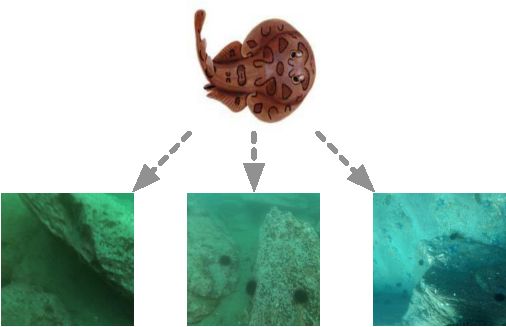
\includegraphics[width=\textwidth]{figures/RUIE_dataset_domain.pdf}
  \caption{RUIE数据集多域转译示例。}
  \label{fig:ruie_domain}
\end{figure*}

如图~\ref{fig:ruie_domain}所示,RUIE数据集进行多样式域转译实验时,选择RUIE的子集UCCS的三种作为水下三个样式域,每种100张,选取EUVP中的100张无水子集作为空中域。在进行测试实验时,选择EUVP中无水域的100张作为空中域,测试训练模型,以测试模型转译到水下多个样式域的效果。

\begin{figure*}[ht]
    \centering
  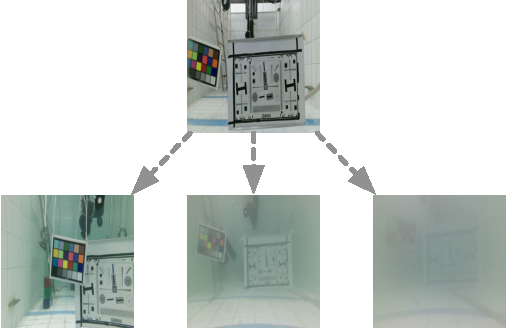
\includegraphics[width=\textwidth]{figures/UVB_dataset_domain.pdf}
  \caption{UVB 2017数据集多域转译示例。}
  \label{fig:uvb_domain}
\end{figure*}

如图~\ref{fig:uvb_domain}所示,Underwater Vision Benchmark 2017(UVB 2017)数据集进行多样式域转译实验时,选择衰减为0中66张作为的空中域,衰减为1.2、1.58、3.0四种样式明显的作为水下样式域。在进行测试时,选择无水中的30张测试模型转译到多样式域的效果。

\begin{figure*}[ht]
    \centering
  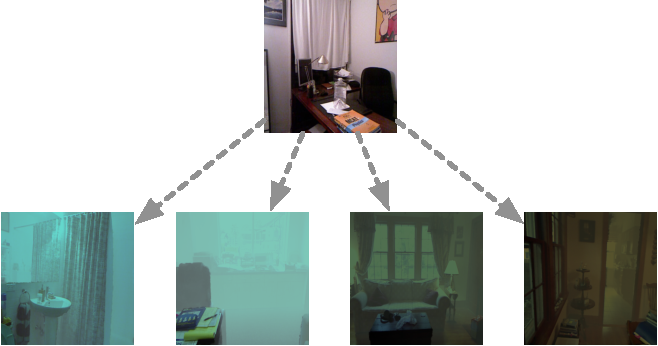
\includegraphics[width=\textwidth]{figures/UWCNN_dataset_domain.pdf}
  \caption{UWCNN数据集多域转译示例。}
  \label{fig:uwcnn_domain}
\end{figure*}

如图~\ref{tab:uwcnn_comparison}所示,UWCNN数据集进行多样式域转译实验时,选择室内图像中249张作为空中域,近海type-1,type-3,type-5,type-7四种较为明显样式的域作为水下多样式域,每个域选择249张。测试时,选择100张进行测试,看模型转译成多多样式域的效果。

\subsection{评价准则}
% 和多样性
为了方便进行质量评价,我们对图像的真实性进行评价。真实性选用Fréchet Inception Distance(FID)来进行评价。FID比较模型生成样本和真实样本统计特性的问题。FID越低,图像质量越好;反之,得分越高,质量越差。较低的FID意味着两个分布之间更接近,也就意味着生成图片的跟真实结果之间相似性较高。在进行多样式域实验中,我们生成的多个域结果与该域真实图像之间计算FID,就可以比较出每个域的生成结果与真实结果之间的相似性。
% 多样性我们选择Learned Perceptual Image Patch Similarity (LPIPS)来评价。预训练好的AlexNet~\cite{krizhevsky2017imagenet}网络来提取特征后计算$L_1$距离,同一个输入的多个结果对之间计算平均距离,对于测试图像求平均值作为LPIPS结果。在进行多样式域转译实验中,输入会转译成多个样式域的结果

另外,还使用水下指标UCIQE和UIQM来验证生成结果的真实性。UCIQE和UIQM都是无参考批评家指标,当生成结果足够真实时,目标域的生成结果和真实样本在这两个指标在色彩、饱和度、对比度上,清晰度等质量上是一致的。通过对比真实样本和合成样本的评价结果,可以看出样本的真实性。


\section{水下图像多样式域合成结果分析}
\subsection{定性结果分析}
\begin{figure*}[htp]
    \centering
  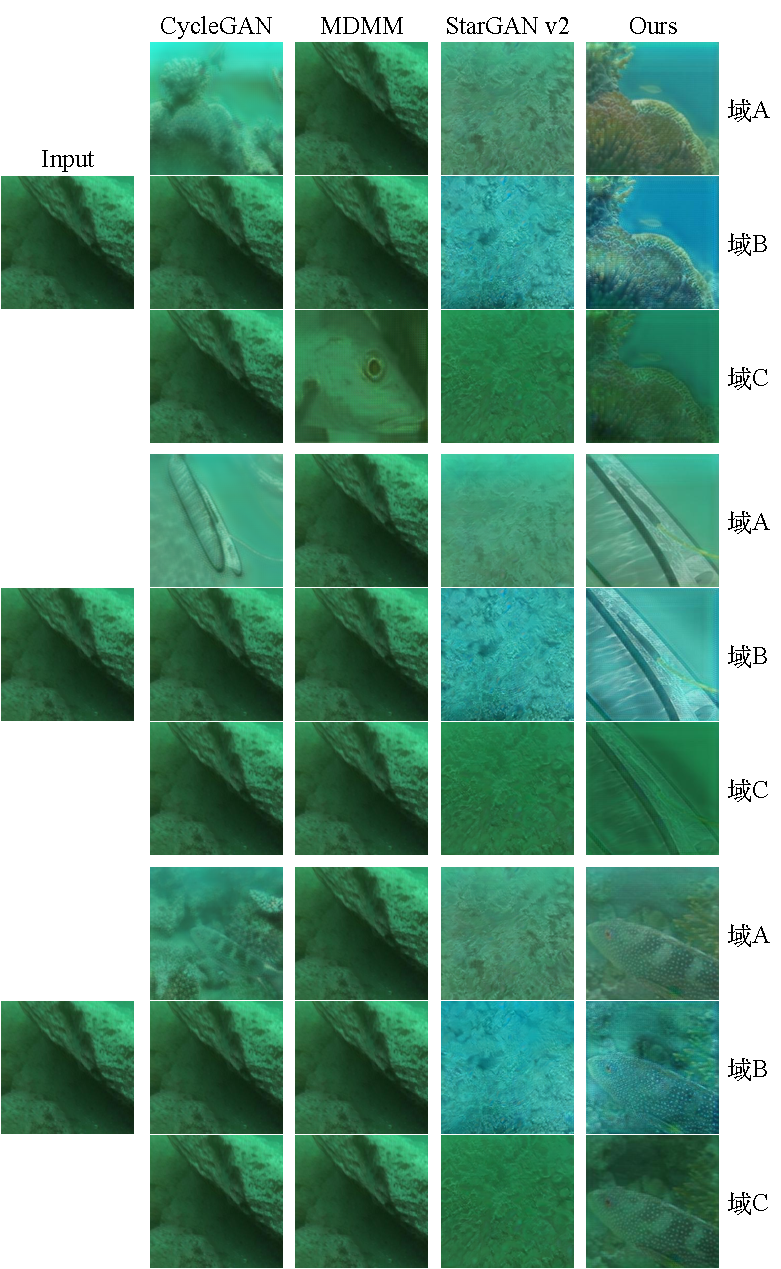
\includegraphics[width=0.9\textwidth]{figures/comparison_ruie_domain.pdf}
  \caption{在RUIE数据集上,基准方法和我们提出的方法在多样式转译任务结果比较。}
  \label{fig:comparison_ruie_domain}
\end{figure*}

图~\ref{fig:comparison_ruie_domain}展示了不同方法在RUIE数据集上的定性结果对比。左边第一列表示模型输入图像,右边每列代表标注方法对应的结果。从对比图中可以看到,CycleGAN、MDMM、StarGAN v2 我们的方法。


\begin{figure*}[htp]
    \centering
  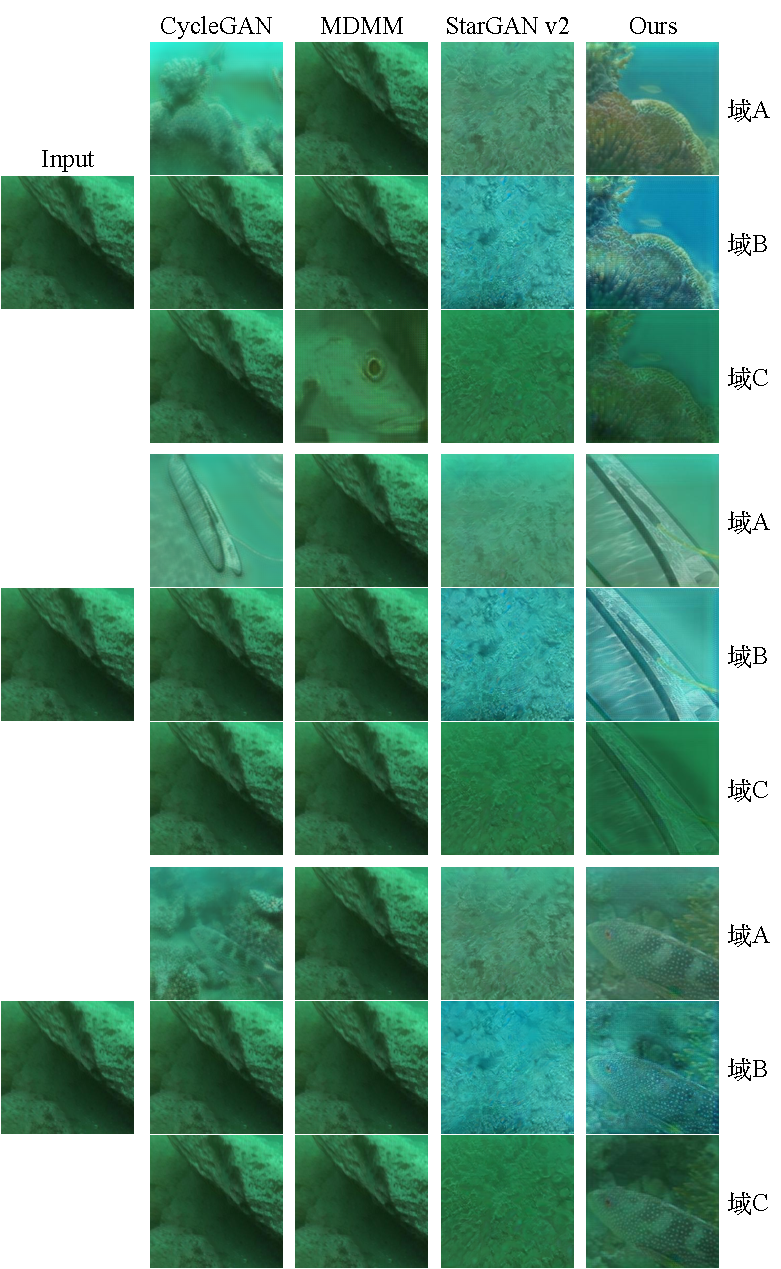
\includegraphics[width=0.9\textwidth]{figures/comparison_ruie_domain.pdf}
  \caption{在UVB 2017数据集上,基准方法和我们提出的方法在多样式转译任务结果比较。}
  \label{fig:comparison_uvb_domain}
\end{figure*}

\begin{figure*}[htp]
    \centering
  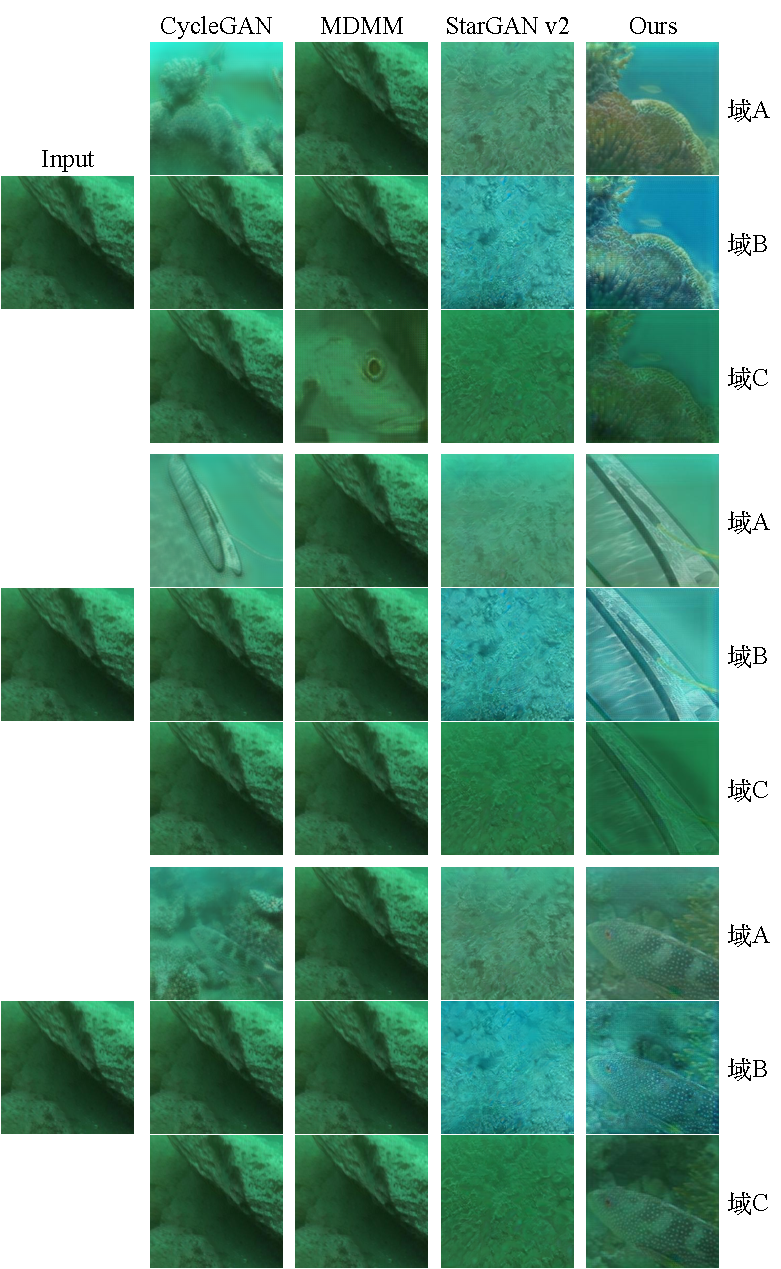
\includegraphics[width=0.9\textwidth]{figures/comparison_ruie_domain.pdf}
  \caption{在UWCNN数据集上,基准方法和我们提出的方法在多样式转译任务结果比较。}
  \label{fig:comparison_uwcnn_domain}
\end{figure*}

\subsection{定量结果分析}
真实性定量指标FID结果表格~\ref{tab:ruie_domain_fid},表格~\ref{tab:uvb_domain_fid}和~\ref{tab:uwcnn_domain_fid}所示。在图像FID质量分析中,我们对比了能完成水下图像多样式域转译的方法CycleGAN、MDMM、StarGAN v2基准方法,在RUIE、UVB 2017、UWCNN数据集上分别进行了测评,测评的基准方法全部来自作者Github给出的完整代码和标准使用方式。通过用FID评价,能够客观的评价各种方法的生成结果。

\begin{table*}[ht]
\centering
\caption{在RUIE数据集上,基准方法和我们方法的真实性FID定量比较。}
  \begin{tabular}{c|ccccccc}
    \hline\noalign{\smallskip}
    FID$\downarrow$ & CycleGAN & MDMM & StarGAN v2 & Ours \\
    \noalign{\smallskip}\hline\noalign{\smallskip}
    Input$\rightarrow$域A & 105.2800 & 154.0302 & 221.6996 & \textbf{82.8535}  \\
    Input$\rightarrow$域B & \textbf{127.3358} & 165.2080 & 160.4444 & 132.0970  \\
    Input$\rightarrow$域C & 99.8060 & 132.0193 & 201.7589 & \textbf{78.8587}  \\
    \noalign{\smallskip}\hline
  \end{tabular}
  \label{tab:ruie_domain_fid}
\end{table*}

表格~\ref{tab:ruie_domain_fid}中,

\begin{table*}[ht]
\centering
\caption{在UVB 2017数据集上,基准方法和我们方法的真实性FID定量比较。}
  \begin{tabular}{c|ccccccc}
    \hline\noalign{\smallskip}
    FID$\downarrow$ & CycleGAN & MDMM & StarGAN v2 & Ours \\
    \noalign{\smallskip}\hline\noalign{\smallskip}
    Input$\rightarrow$域A & 231.2559 & 308.1764 & 132.5135 & \textbf{123.4455}  \\
    Input$\rightarrow$域B & \textbf{203.3703} & 277.9446 & 261.4843 & 249.0746  \\
    Input$\rightarrow$域C & \textbf{137.9410} & 249.9113 & 203.4555 & 186.2838  \\
    \noalign{\smallskip}\hline
  \end{tabular}
  \label{tab:uvb_domain_fid}
\end{table*}

\begin{table*}[ht]
\centering
\caption{在UWCNN数据集上,基准方法和我们方法的真实性FID定量比较。}
  \begin{tabular}{c|ccccccc}
    \hline\noalign{\smallskip}
    FID$\downarrow$ & CycleGAN & MDMM & StarGAN v2 & Ours \\
    \noalign{\smallskip}\hline\noalign{\smallskip}
    Input$\rightarrow$域A & 141.4799 & 213.1867 & 216.8333 & \textbf{120.0408}  \\
    Input$\rightarrow$域B & 132.0554 & 167.2517 & 168.5740 & \textbf{116.5354}  \\
    Input$\rightarrow$域C & 116.4376 & 158.9736 & 150.5446 & \textbf{98.0187}  \\
    Input$\rightarrow$域D & \textbf{72.5141}  & 136.5694 & 114.0044 & 72.6410  \\
    \noalign{\smallskip}\hline
  \end{tabular}
  \label{tab:uwcnn_domain_fid}
\end{table*}

\subsection{消融实验}

\chapter{总结与展望}
\section{全文总结}
本文主要对水下图像的多样式合成问题进行了深入的探讨,通过对图像转译工作进行研究,对于图像转译工作的多模态转译和多域转译方向开展实验,尝试通过提出两种不同的思路的模型进行解决。本文主要工作如下:

\begin{itemize}
	\item [1.]
	本文对生成对抗网络进行了研究,了解现有基于生成对抗网络的的图像转译问题的国内外现状,对于生成对抗网络在图像合成上的思路进行梳理。水下图像数据在水下视觉研究中非常重要,本文调研了水下图成像以及水下图像特点,对水下数据和评价进行了了解,通过对水下图像合成方法综述,总结了水下图像多样式合成的方法以及各自特点。
	
	\item [2.]
	针对水下图像多样式合成的问题,基于对生成对抗网络上的图像转译研究,我们梳理了水下图像多样式合成的两种思路,一种是基于跨域图像多模态转译方法,将多个水下样式看作水下域的多个模态进行处理,通过引入内容一致性损失限制合成过程中内容保持完整不损耗;另一种是基于多域转译方法,将各个样式看作多个域来进行处理,通过样式编码控制到各个域的合成。并在这两种思路上进行网络模型结构设计和目标函数设置。

	\item [3.]
	对于以上提出的水下图像多样式转译的两种思路,我们在图像转译问题中找到最经典和最前沿的方法,对各自思路在多个合成数据集和真实水下数据集上设计了一系列的对比实验和消融实验。我们的评价指标充分选取了图像转译中评价指标和水下图像研究的评价指标,保证在评价过程中足够充分和客观,另外在定性视觉结果和定量指标结果上进行了详细分析,从而验证了我们提出网络结构对于该问题能够有效的解决和其优越性。

\end{itemize}

\section{讨论}
尽管我们提出的两种思路以及对应的两种模型结构都可以出色地解决合成水下多样式转译问题,但是目前基准方法和我们提出的基于生成对抗网络的水下图像多样式合成工作对训练数据有着较高的要求,也是由于基于大量数据的图像转译方法自身必然会收到数据的限制,在多个不同数据集上,模型训练结果有较大差异,虽然数据自身可以无需配对,但是训练数据中不纯净存在扰乱的数据或特定图像转译任务较难时,部分水下图像多样式合成工作会出现转译失败的案例。




%%% 其它部分
% \backmatter

%% 本科生要这几个索引,研究生不要。选择性留下。
% 插图索引
% \listoffigures
% 表格索引
% \listoftables
% 公式索引
% \listofequations


%% 参考文献
% 注意:至少需要引用一篇参考文献,否则下面两行可能引起编译错误。
% 如果不需要参考文献,请将下面两行删除或注释掉。
\bibliographystyle{thuthesis}
% \clearpage %目录中显示的页码正确
% \phantomsection %目录中的链接能正确跳转
% \addcontentsline{toc}{chapter}{参考文献} %目录中以章的名义添加条目
\bibliography{ref/refs}


%% 附录
% \begin{appendix}
% \chapter{外文资料原文}
\label{cha:engorg}

\title{The title of the English paper}

\textbf{Abstract:} As one of the most widely used techniques in operations
research, \emph{ mathematical programming} is defined as a means of maximizing a
quantity known as \emph{bjective function}, subject to a set of constraints
represented by equations and inequalities. Some known subtopics of mathematical
programming are linear programming, nonlinear programming, multiobjective
programming, goal programming, dynamic programming, and multilevel
programming$^{[1]}$.

It is impossible to cover in a single chapter every concept of mathematical
programming. This chapter introduces only the basic concepts and techniques of
mathematical programming such that readers gain an understanding of them
throughout the book$^{[2,3]}$.


\section{Single-Objective Programming}
The general form of single-objective programming (SOP) is written
as follows,
\begin{equation}\tag*{(123)} % 如果附录中的公式不想让它出现在公式索引中,那就请
                             % 用 \tag*{xxxx}
\left\{\begin{array}{l}
\max \,\,f(x)\\[0.1 cm]
\mbox{subject to:} \\ [0.1 cm]
\qquad g_j(x)\le 0,\quad j=1,2,\cdots,p
\end{array}\right.
\end{equation}
which maximizes a real-valued function $f$ of
$x=(x_1,x_2,\cdots,x_n)$ subject to a set of constraints.

\newtheorem{mpdef}{Definition}[chapter]
\begin{mpdef}
In SOP, we call $x$ a decision vector, and
$x_1,x_2,\cdots,x_n$ decision variables. The function
$f$ is called the objective function. The set
\begin{equation}\tag*{(456)} % 这里同理,其它不再一一指定。
S=\left\{x\in\Re^n\bigm|g_j(x)\le 0,\,j=1,2,\cdots,p\right\}
\end{equation}
is called the feasible set. An element $x$ in $S$ is called a
feasible solution.
\end{mpdef}

\newtheorem{mpdefop}[mpdef]{Definition}
\begin{mpdefop}
A feasible solution $x^*$ is called the optimal
solution of SOP if and only if
\begin{equation}
f(x^*)\ge f(x)
\end{equation}
for any feasible solution $x$.
\end{mpdefop}

One of the outstanding contributions to mathematical programming was known as
the Kuhn-Tucker conditions\ref{eq:ktc}. In order to introduce them, let us give
some definitions. An inequality constraint $g_j(x)\le 0$ is said to be active at
a point $x^*$ if $g_j(x^*)=0$. A point $x^*$ satisfying $g_j(x^*)\le 0$ is said
to be regular if the gradient vectors $\nabla g_j(x)$ of all active constraints
are linearly independent.

Let $x^*$ be a regular point of the constraints of SOP and assume that all the
functions $f(x)$ and $g_j(x),j=1,2,\cdots,p$ are differentiable. If $x^*$ is a
local optimal solution, then there exist Lagrange multipliers
$\lambda_j,j=1,2,\cdots,p$ such that the following Kuhn-Tucker conditions hold,
\begin{equation}
\label{eq:ktc}
\left\{\begin{array}{l}
    \nabla f(x^*)-\sum\limits_{j=1}^p\lambda_j\nabla g_j(x^*)=0\\[0.3cm]
    \lambda_jg_j(x^*)=0,\quad j=1,2,\cdots,p\\[0.2cm]
    \lambda_j\ge 0,\quad j=1,2,\cdots,p.
\end{array}\right.
\end{equation}
If all the functions $f(x)$ and $g_j(x),j=1,2,\cdots,p$ are convex and
differentiable, and the point $x^*$ satisfies the Kuhn-Tucker conditions
(\ref{eq:ktc}), then it has been proved that the point $x^*$ is a global optimal
solution of SOP.

\subsection{Linear Programming}
\label{sec:lp}

If the functions $f(x),g_j(x),j=1,2,\cdots,p$ are all linear, then SOP is called
a {\em linear programming}.

The feasible set of linear is always convex. A point $x$ is called an extreme
point of convex set $S$ if $x\in S$ and $x$ cannot be expressed as a convex
combination of two points in $S$. It has been shown that the optimal solution to
linear programming corresponds to an extreme point of its feasible set provided
that the feasible set $S$ is bounded. This fact is the basis of the {\em simplex
  algorithm} which was developed by Dantzig as a very efficient method for
solving linear programming.
\begin{table}[ht]
\centering
  \centering
  \caption*{Table~1\hskip1em This is an example for manually numbered table, which
    would not appear in the list of tables}
  \label{tab:badtabular2}
  \begin{tabular}[c]{|m{1.5cm}|c|c|c|c|c|c|}\hline
    \multicolumn{2}{|c|}{Network Topology} & \# of nodes &
    \multicolumn{3}{c|}{\# of clients} & Server \\\hline
    GT-ITM & Waxman Transit-Stub & 600 &
    \multirow{2}{2em}{2\%}&
    \multirow{2}{2em}{10\%}&
    \multirow{2}{2em}{50\%}&
    \multirow{2}{1.2in}{Max. Connectivity}\\\cline{1-3}
    \multicolumn{2}{|c|}{Inet-2.1} & 6000 & & & &\\\hline
    \multirow{2}{1.5cm}{Xue} & Rui  & Ni &\multicolumn{4}{c|}{\multirow{2}*{\thuthesis}}\\\cline{2-3}
    & \multicolumn{2}{c|}{ABCDEF} &\multicolumn{4}{c|}{} \\\hline
\end{tabular}
\end{table}

Roughly speaking, the simplex algorithm examines only the extreme points of the
feasible set, rather than all feasible points. At first, the simplex algorithm
selects an extreme point as the initial point. The successive extreme point is
selected so as to improve the objective function value. The procedure is
repeated until no improvement in objective function value can be made. The last
extreme point is the optimal solution.

\subsection{Nonlinear Programming}

If at least one of the functions $f(x),g_j(x),j=1,2,\cdots,p$ is nonlinear, then
SOP is called a {\em nonlinear programming}.

A large number of classical optimization methods have been developed to treat
special-structural nonlinear programming based on the mathematical theory
concerned with analyzing the structure of problems.
\begin{figure}[h]
  \centering
  \includegraphics{thu-lib-logo}
  \caption*{Figure~1\quad This is an example for manually numbered figure,
    which would not appear in the list of figures}
  \label{tab:badfigure2}
\end{figure}

Now we consider a nonlinear programming which is confronted solely with
maximizing a real-valued function with domain $\Re^n$.  Whether derivatives are
available or not, the usual strategy is first to select a point in $\Re^n$ which
is thought to be the most likely place where the maximum exists. If there is no
information available on which to base such a selection, a point is chosen at
random. From this first point an attempt is made to construct a sequence of
points, each of which yields an improved objective function value over its
predecessor. The next point to be added to the sequence is chosen by analyzing
the behavior of the function at the previous points. This construction continues
until some termination criterion is met. Methods based upon this strategy are
called {\em ascent methods}, which can be classified as {\em direct methods},
{\em gradient methods}, and {\em Hessian methods} according to the information
about the behavior of objective function $f$. Direct methods require only that
the function can be evaluated at each point. Gradient methods require the
evaluation of first derivatives of $f$. Hessian methods require the evaluation
of second derivatives. In fact, there is no superior method for all
problems. The efficiency of a method is very much dependent upon the objective
function.

\subsection{Integer Programming}

{\em Integer programming} is a special mathematical programming in which all of
the variables are assumed to be only integer values. When there are not only
integer variables but also conventional continuous variables, we call it {\em
  mixed integer programming}. If all the variables are assumed either 0 or 1,
then the problem is termed a {\em zero-one programming}. Although integer
programming can be solved by an {\em exhaustive enumeration} theoretically, it
is impractical to solve realistically sized integer programming problems. The
most successful algorithm so far found to solve integer programming is called
the {\em branch-and-bound enumeration} developed by Balas (1965) and Dakin
(1965). The other technique to integer programming is the {\em cutting plane
  method} developed by Gomory (1959).

\hfill\textit{Uncertain Programming\/}\quad(\textsl{BaoDing Liu, 2006.2})

\section*{References}
\noindent{\itshape NOTE: These references are only for demonstration. They are
  not real citations in the original text.}

\begin{translationbib}
\item Donald E. Knuth. The \TeX book. Addison-Wesley, 1984. ISBN: 0-201-13448-9
\item Paul W. Abrahams, Karl Berry and Kathryn A. Hargreaves. \TeX\ for the
  Impatient. Addison-Wesley, 1990. ISBN: 0-201-51375-7
\item David Salomon. The advanced \TeX book.  New York : Springer, 1995. ISBN:0-387-94556-3
\end{translationbib}

\chapter{外文资料的调研阅读报告或书面翻译}

\title{英文资料的中文标题}

{\heiti 摘要:} 本章为外文资料翻译内容。如果有摘要可以直接写上来,这部分好像没有
明确的规定。

\section{单目标规划}
北冥有鱼,其名为鲲。鲲之大,不知其几千里也。化而为鸟,其名为鹏。鹏之背,不知其几
千里也。怒而飞,其翼若垂天之云。是鸟也,海运则将徙于南冥。南冥者,天池也。
\begin{equation}\tag*{(123)}
 p(y|\mathbf{x}) = \frac{p(\mathbf{x},y)}{p(\mathbf{x})}=
\frac{p(\mathbf{x}|y)p(y)}{p(\mathbf{x})}
\end{equation}

吾生也有涯,而知也无涯。以有涯随无涯,殆已!已而为知者,殆而已矣!为善无近名,为
恶无近刑,缘督以为经,可以保身,可以全生,可以养亲,可以尽年。

\subsection{线性规划}
庖丁为文惠君解牛,手之所触,肩之所倚,足之所履,膝之所倚,砉然响然,奏刀騞然,莫
不中音,合于桑林之舞,乃中经首之会。
\begin{table}[ht]
\centering
  \centering
  \caption*{表~1\hskip1em 这是手动编号但不出现在索引中的一个表格例子}
  \label{tab:badtabular3}
  \begin{tabular}[c]{|m{1.5cm}|c|c|c|c|c|c|}\hline
    \multicolumn{2}{|c|}{Network Topology} & \# of nodes &
    \multicolumn{3}{c|}{\# of clients} & Server \\\hline
    GT-ITM & Waxman Transit-Stub & 600 &
    \multirow{2}{2em}{2\%}&
    \multirow{2}{2em}{10\%}&
    \multirow{2}{2em}{50\%}&
    \multirow{2}{1.2in}{Max. Connectivity}\\\cline{1-3}
    \multicolumn{2}{|c|}{Inet-2.1} & 6000 & & & &\\\hline
    \multirow{2}{1.5cm}{Xue} & Rui  & Ni &\multicolumn{4}{c|}{\multirow{2}*{\thuthesis}}\\\cline{2-3}
    & \multicolumn{2}{c|}{ABCDEF} &\multicolumn{4}{c|}{} \\\hline
\end{tabular}
\end{table}

文惠君曰:“嘻,善哉!技盖至此乎?”庖丁释刀对曰:“臣之所好者道也,进乎技矣。始臣之
解牛之时,所见无非全牛者;三年之后,未尝见全牛也;方今之时,臣以神遇而不以目视,
官知止而神欲行。依乎天理,批大郤,导大窾,因其固然。技经肯綮之未尝,而况大坬乎!
良庖岁更刀,割也;族庖月更刀,折也;今臣之刀十九年矣,所解数千牛矣,而刀刃若新发
于硎。彼节者有间而刀刃者无厚,以无厚入有间,恢恢乎其于游刃必有余地矣。是以十九年
而刀刃若新发于硎。虽然,每至于族,吾见其难为,怵然为戒,视为止,行为迟,动刀甚微,
謋然已解,如土委地。提刀而立,为之而四顾,为之踌躇满志,善刀而藏之。”

文惠君曰:“善哉!吾闻庖丁之言,得养生焉。”


\subsection{非线性规划}
孔子与柳下季为友,柳下季之弟名曰盗跖。盗跖从卒九千人,横行天下,侵暴诸侯。穴室枢
户,驱人牛马,取人妇女。贪得忘亲,不顾父母兄弟,不祭先祖。所过之邑,大国守城,小
国入保,万民苦之。孔子谓柳下季曰:“夫为人父者,必能诏其子;为人兄者,必能教其弟。
若父不能诏其子,兄不能教其弟,则无贵父子兄弟之亲矣。今先生,世之才士也,弟为盗
跖,为天下害,而弗能教也,丘窃为先生羞之。丘请为先生往说之。”
\begin{figure}[h]
  \centering
  \includegraphics{thu-whole-logo}
  \caption*{图~1\hskip1em 这是手动编号但不出现索引中的图片的例子}
  \label{tab:badfigure3}
\end{figure}

柳下季曰:“先生言为人父者必能诏其子,为人兄者必能教其弟,若子不听父之诏,弟不受
兄之教,虽今先生之辩,将奈之何哉?且跖之为人也,心如涌泉,意如飘风,强足以距敌,
辩足以饰非。顺其心则喜,逆其心则怒,易辱人以言。先生必无往。”

孔子不听,颜回为驭,子贡为右,往见盗跖。

\subsection{整数规划}
盗跖乃方休卒徒大山之阳,脍人肝而餔之。孔子下车而前,见谒者曰:“鲁人孔丘,闻将军
高义,敬再拜谒者。”谒者入通。盗跖闻之大怒,目如明星,发上指冠,曰:“此夫鲁国之
巧伪人孔丘非邪?为我告之:尔作言造语,妄称文、武,冠枝木之冠,带死牛之胁,多辞缪
说,不耕而食,不织而衣,摇唇鼓舌,擅生是非,以迷天下之主,使天下学士不反其本,妄
作孝弟,而侥幸于封侯富贵者也。子之罪大极重,疾走归!不然,我将以子肝益昼餔之膳。”


\chapter{其它附录}
前面两个附录主要是给本科生做例子。其它附录的内容可以放到这里,当然如果你愿意,可
以把这部分也放到独立的文件中,然后将其 \cs{input} 到主文件中。

% \end{appendix}

%% 致谢
% 如果使用声明扫描页,将可选参数指定为扫描后的 PDF 文件名,例如:
% \begin{acknowledgement}[scan-statement.pdf]
\begin{acknowledgement}
  衷心感谢导师对本人的悉心指导,以及在学习和生活上的支持、鼓励和帮助!

\end{acknowledgement}


%% 个人简历
\begin{resume}

  \resumeitem{个人简历}

  1996年1月22日出生于山东省滨州市。

  2014年9月考入山东师范大学物理与电子科学学院学院电子信息科学与技术专业,2018年6月本科毕业并获得理学学士学位。
  
  2018年9月考入中国海洋大学大学信息科学与工程学院通信与信息系统专业攻读硕士学位至今。

  \researchitem{发表的学术论文} % 发表的和录用的合在一起

  % 1. 已经刊载的学术论文(本人是第一作者,或者导师为第一作者本人是第二作者)
  \begin{publications}
    \item XXX X, XXX X, XXX X, et al., Title XXX, IEEE XXX, vol. X, pp. XXX-XXX, 20XX.(SCI/EI XXX)
  \end{publications}

  % 2. 尚未刊载,但已经接到正式录用函的学术论文(本人为第一作者,或者
  %    导师为第一作者本人是第二作者)。
  \begin{publications}[before=\publicationskip,after=\publicationskip]
    \item XXX X, XXX X, XXX X, et al., Title XXX, IEEE XXX, vol. X, pp. XXX-XXX, 20XX.(SCI/EI XXX)
  \end{publications}

  % 3. 其他学术论文。可列出除上述两种情况以外的其他学术论文,但必须是
  %    已经刊载或者收到正式录用函的论文。
  \begin{publications}
    \item XXX X, XXX X, XXX X, et al., Title XXX, IEEE XXX, vol. X, pp. XXX-XXX, 20XX.(SCI/EI XXX)
  \end{publications}

  \researchitem{在学期间参加的研究项目} % 有就写,没有就删除
  \begin{achievements}
    \item 国家自然科学基金面上项目“ 类别不平衡条件下海洋浮游生物图像精细识别及其原位应用研究”(批准号:61771440)
    \item 国家自然科学基金面上项目“ 海洋中小型浮游生物原位光学观测关键技术研究”(批准号:41776113)

  \end{achievements}

\end{resume}


%% 本科生进行格式审查是需要下面这个表格,答辩可能不需要。选择性留下。
% 综合论文训练记录表
%\includepdf[pages=-]{scan-record.pdf}
\end{document}
